\documentclass[10pt]{article}

\usepackage[table,xcdraw]{xcolor}
\usepackage[utf8]{inputenc}
\usepackage{tabularx}
\usepackage{hyperref}
\usepackage{array}
\usepackage{graphicx} % Per inserire immagini (loghi)
\usepackage{geometry} % Per personalizzare i margini
\usepackage{fancyhdr} % Per gestire intestazioni e piè di pagina
\usepackage{tikz}
\usepackage{pgfplots}
\usepackage{pgf-pie}
\usepackage{ragged2e}
\usepackage{anyfontsize}
\usepackage{tabularx, etoolbox}
\usepackage{eso-pic} % Per aggiungere elementi grafici su tutte le pagine
\usepackage{float}
\usepackage{setspace}
\usepackage{longtable}
\usepackage{listings}
\usepackage{lstautogobble}
\usepackage[framemethod=TikZ]{mdframed}
\usepackage{xcolor}
\usepackage{adjustbox}


% Minimal color setup
\definecolor{MLbg}{HTML}{F8F9FA}
\definecolor{MLborder}{HTML}{E6E6E6}
\definecolor{MLstring}{HTML}{D12F1B}
\definecolor{MLcomment}{HTML}{656565}
\definecolor{MLkeyword}{HTML}{703DAA}
\definecolor{MLidentifier}{HTML}{000000}

\mdfsetup{
    linewidth=1pt,
    linecolor=MLborder,
    backgroundcolor=MLbg,
    roundcorner=4pt,
    skipabove=\baselineskip
}

\lstset{
    framesep=0pt,
    basicstyle=\ttfamily\small,
    columns=flexible,
    breaklines=true,
    tabsize=8,
    % keepspaces=true,
    showstringspaces=false,
    commentstyle=\color{MLcomment},
    keywordstyle=\color{MLkeyword},
    stringstyle=\color{MLstring},
    numbers=left,
    numberstyle=\tiny\color{MLcomment},
    numbersep=0pt, % Riduce lo spazio tra i numeri e il codice
    xleftmargin=-2em,
    aboveskip=0pt, % Riduce lo spazio sopra il codice
    belowskip=0pt, % Riduce lo spazio sotto il codice
}

\surroundwithmdframed{lstlisting}

\newcommand\version{0.1.7} %aggiunta versione come variabile
\newcommand{\myparagraph}[1]{\paragraph{#1}\mbox{}\\}
\newcommand{\mysubparagraph}[1]{\subparagraph{#1}\mbox{}\\}

\graphicspath{{images/}}
%\graphicspath{{../images/}}

\setcounter{secnumdepth}{5}
\setcounter{tocdepth}{4}

%cambio misure della pagina
\geometry{a4paper,left=25mm,right=25mm,top=25mm,bottom=25mm}
\setlength{\parindent}{0pt}
\definecolor{colorePie}{HTML}{ebdfc7}
\pagestyle{fancy}
\fancyhf{}
\renewcommand{\headrulewidth}{0.4pt}
\lhead{
    \parbox[c]{1cm}{\includegraphics[width=1.1cm]{Sevenbitslogo.png}}
}
\rhead{\textcolor[HTML]{9e978a}{ SPECIFICA TECNICA v\version}
}
\setlength{\headheight}{25pt}
\cfoot{\thepage}

\renewcommand*\contentsname{Indice}
\renewcommand{\listfigurename}{Elenco delle figure}
\renewcommand{\listtablename}{Elenco delle tabelle}

\begin{document}

% Pagina del titolo
\begin{titlepage}
    \setcounter{page}{0}
    \centering
    % Inserisci il logo del gruppo (modifica il percorso dell'immagine)
    \includegraphics[width=7.2cm]{Sevenbitslogo.png} \\[2cm]

    % Titolo
    {\fontsize{40}{40}\bfseries Specifica Tecnica}\selectfont \\[3.9em]

    % Sottotitolo
    {\huge NearYou\\ \vspace{3mm }Smart custom advertising platform} \\[2.7em]

    % Email del gruppo
    {\large sevenbits.swe.unipd@gmail.com} \\[3em]

    % Spazio per il logo dell'università
    \hfill

    \AddToShipoutPictureBG{ % Imposta il triangolo con logo
        \ifnum\value{page}=0
        \begin{tikzpicture}[overlay]

            % Definisce un triangolo blu in basso a destra
            \fill[colorePie]
                (current page.south east) -- ++(-9cm,0) -- ++(9cm,9cm);

            % Inserisce il logo all'interno del triangolo
            \node[anchor=south east, xshift=-0.3cm, yshift=0.3cm] at (current page.south east) {
                \includegraphics[width=4.5cm]{LogoUnipd.png}
            };
        \end{tikzpicture}
        \fi
    }

\vfill % Aggiunge spazio verticale per centrare il contenuto
\end{titlepage}
\newpage
\clearpage
\setcounter{page}{1}

% Registro Modifiche
\begin{center}
\textbf{Registro modifiche}\\
\end{center}

\renewcommand{\arraystretch}{1.5}
\rowcolors{0}{gray!11}{white} % Aggiunge colore alternato alle righe

\begin{longtable}{|>{\centering\arraybackslash}m{1.5cm}|>{\centering\arraybackslash}m{2cm}|>{\centering\arraybackslash}m{2.5cm}|>{\centering\arraybackslash}m{2.5cm}|>{\centering\arraybackslash}m{5cm}|}
\hline
\textbf{Versione} & \textbf{Data} & \textbf{Autore} & \textbf{Verificatore} & \textbf{Descrizione}\\
\endhead
    \hline
    0.2.0 & 2025-03-28 & Uncas Peruzzi & Riccardo Pivetta & Refactoring Struttura, Aggiunti SimulationService e PositionToMessageService \\
    \hline
    0.1.10 & 2025-03-28 & Riccardo Piva & Federico Pivetta & refactor sezione ClickHouse e Grafana architettura di sistema\\
    \hline
    0.1.9 & 2025-03-28 & Uncas Peruzzi & Federico Pivetta & Aggiunte immagini servizi e diagrammi UML \\
    \hline
    0.1.8 & 2025-03-22 & Alfredo Rubino & Uncas Peruzzi & Aggiunto pattern Adapter \\
    \hline
    0.1.7 & 2025-03-22 & Federico Pivetta & Uncas Peruzzi & Ampliati i paragrafi per i pattern Strategy e Factory \\
    \hline
    0.1.6 & 2025-03-21 & Riccardo Piva & Uncas Peruzzi & Sezione Integrazione Architettura logica e Architettura di sistema \\
    \hline
    0.1.5 & 2025-03-17 & Riccardo Piva & Alfredo Rubino & Fix generali e miglioramenti \\
    \hline
    0.1.4 & 2025-03-16 & Riccardo Piva & Alfredo Rubino & Redazione generale macro sezioni documento \\
    \hline
    0.1.3 & 2025-03-05 & Alfredo Rubino & Manuel Gusella & Redazione sottosezione \hyperref[sec:strumenti]{Strumenti e Servizi} della sezione Tecnologie\\
    \hline
    0.1.2 & 2025-03-05 & Leonardo Trolese & Manuel Gusella & Conclusione redazione sottosezione \hyperref[sec:linguaggi]{Panoramica dei Linguaggi} della sezione Tecnologie\\
    \hline
    0.1.1 & 2025-03-02 & Leonardo Trolese & Manuel Gusella & Redazione sottosezione \hyperref[sec:linguaggi]{Panoramica dei Linguaggi} della sezione Tecnologie\\
    \hline
    0.1.0 & 2025-02-26 & Leonardo Trolese & Manuel Gusella & Inizio redazione del documento\\
    \hline
\end{longtable}
\rowcolors{0}{}{} % Riporta le righe alla colorazione originale

\newpage
\tableofcontents
\newpage
\listoffigures %elenco delle figure sarà da usare per ogni immagine
\newpage
\listoftables %lista delle tabelle presenti nel documento
\newpage
% \begin{justify}

\section{Introduzione}
\subsection{Scopo del documento}
Il presente documento si propone come una risorsa completa per la comprensione degli aspetti tecnici e progettuali della piattaforma "NearYou", dedicata alla
creazione di soluzioni di advertising personalizzato tramite intelligenza artificiale. L’obiettivo principale è fornire una descrizione dettagliata dell’architettura
implementativa e di deployment, illustrando le tecnologie adottate e le motivazioni alla base delle scelte progettuali.\\
Nel contesto dell'architettura implementativa, il documento analizza nel dettaglio i moduli principali del sistema, i design pattern utilizzati. Saranno inclusi
diagrammi delle classi, e una spiegazione dettagliata dei design pattern utilizzati e delle motivazioni di queste scelte.\\
Gli obiettivi di questo documento sono: motivare le decisioni architetturali, fungere da guida per lo sviluppo della piattaforma, e garantire la piena tracciabilità e
copertura dei requisiti definiti nel documento di \textit{Analisi dei Requisiti\_v1.0.0}.\\
In sintesi, il documento intende essere un punto di riferimento essenziale per tutti gli attori coinvolti nel ciclo di vita del progetto, offrendo una visione chiara e
strutturata delle fondamenta tecniche che sorreggono NearYou e delle logiche che ne determinano il funzionamento.\\

\subsection{Glossario}
Con l'intento di evitare ambiguità interpretative del linguaggio utilizzato, viene fornito un Glossario che si occupa di esplicitare il significato dei termini che riguardano il contesto del Progetto$_G$. I termini presenti nel glossario sono contrassegnati con una \textit{G} a pedice : Termine$_G$.\\
I termini composti, oltre alla $_G$ a pedice, saranno uniti da un "-" come segue: termine-composto$_G$.\\
Le definizioni sono presenti nell'apposito documento \textit{Glossario\_v1.0.0.pdf}.

\subsection{Riferimenti}
\subsubsection{Riferimenti normativi}
\begin{itemize}
    \item[-] Regolamento del Progetto$_G$ didattico  \\
    \textcolor{blue}{\texttt{\url{https://www.math.unipd.it/~tullio/IS-1/2024/Dispense/PD1.pdf}}}\\ (Consultato: 2025-02-10).
    \item[-] Capitolato$_G$ C4 - NearYou - Smart custom advertising platform\\
    \textcolor{blue}{\texttt{\url{https://www.math.unipd.it/~tullio/IS-1/2024/Progetto/C4p.pdf}}}\\ (Consultato: 2025-02-10).
    \item[-] \textit{Norme\_di\_Progetto\_v1.0.0}
\end{itemize}

\subsubsection{Riferimenti informativi}
\begin{itemize}
    \item[-] \textit{Glossario\_v1.0.0}
    \item[-] \textit{Analisi\_dei\_Requisiti\_v1.0.0}
    \item[-] Analisi-dei-Requisiti$_G$ - SWE 2024-25\\
    \textcolor{blue}{\texttt{\url{https://www.math.unipd.it/\~tullio/IS-1/2024/Dispense/T05.pdf}}}\\ (Consultato: 2025-02-10).

    \item[-] Dependency Injection - SWE 2024-25\\
    \textcolor{blue}{\texttt{\url{https://www.math.unipd.it/\~rcardin/swea/2022/Design\%20Pattern\%20Architetturali\%20-\%20Dependency\%20Injection.pdf}}}\\ (Consultato: 2025-02-26).

    \item[-] Design Pattern Creazionali - SWE 2024-25\\
    \textcolor{blue}{\texttt{\url{https://www.math.unipd.it/\~rcardin/swea/2022/Design\%20Pattern\%20Creazionali.pdf}}}\\ (Consultato: 2025-02-26).

    \item[-] Design Pattern Strutturali - SWE 2024-25\\
    \textcolor{blue}{\url{https://www.math.unipd.it/\~rcardin/swea/2022/Design\%20Pattern\%20Strutturali.pdf}}\\ (Consultato: 2025-02-26).

    \item[-] Software Architecture Patterns - SWE 2024-25\\
    \textcolor{blue}{\url{https://www.math.unipd.it/\~rcardin/swea/2022/Software\%20Architecture\%20Patterns.pdf}}\\ (Consultato: 2025-02-26).

    \item[-] Verbali Interni
    \item[-] Verbali Esterni
\end{itemize}


\section{Tecnologie}
Questa sezione descrive le tecnologie utilizzate per lo sviluppo del sistema NearYou, presentando una panoramica degli strumenti, dei linguaggi e dei servizi impiegati, con le motivazioni alla base delle scelte effettuate.

\subsection{Panoramica tecnologica}
Il sistema NearYou si basa su un'architettura a microservizi event-driven che utilizza diverse tecnologie integrate:

\begin{itemize}
    \item \textbf{Python}: Linguaggio principale per lo sviluppo dei componenti del sistema;
    \item \textbf{Apache Kafka}: Sistema di messaggistica distribuito per la comunicazione tra componenti;
    \item \textbf{Apache Flink}: Framework di elaborazione dati in tempo reale;
    \item \textbf{ClickHouse}: Database colonnare ad alte prestazioni;
    \item \textbf{Grafana}: Piattaforma di visualizzazione dei dati in tempo reale;
    \item \textbf{Docker}: Sistema di containerizzazione per il deployment.
\end{itemize}

\subsection{Linguaggi di programmazione}
\label{sec:linguaggi}

\subsubsection{Python}
Linguaggio di programmazione ad alto livello, interpretato e orientato agli oggetti, scelto per la sua leggibilità, la vasta libreria standard e il ricco ecosistema di framework disponibili, particolarmente adatto allo sviluppo rapido di applicazioni.

\myparagraph{Specifiche}
\begin{itemize}
    \item \textbf{Versione}: 3.12.2;
    \item \textbf{Documentazione}: \textcolor{blue}{\url{https://docs.python.org/}} (Consultato: 2025-03-02).
\end{itemize}

\myparagraph{Ruolo nel progetto}
Nel contesto di NearYou, Python viene impiegato per:
\begin{itemize}
    \item[-] Sviluppo di un simulatore per gli spostamenti di più utenti;
    \item[-] Implementazione della logica di elaborazione dati;
    \item[-] Interazione con i servizi esterni e le API;
    \item[-] Gestione della persistenza dei dati;
    \item[-] Applicazione degli algoritmi di selezione dei POI rilevanti.
\end{itemize}

\myparagraph{Dipendenze}
\begin{itemize}
    \item[-] \textbf{ClickHouse Connect}:
    \begin{itemize}
        \item \textbf{Descrizione}: Libreria client per l'interazione con il database ClickHouse, permettendo operazioni di query e gestione dei dati;
        \item \textbf{Versione}: 0.6.8;
        \item \textbf{Documentazione}: \textcolor{blue}{\url{https://clickhouse.com/docs/integrations/python}} (Consultato: 2025-03-02).
    \end{itemize}

    \item[-] \textbf{PyFlink}:
    \begin{itemize}
        \item \textbf{Descrizione}: API Python di Apache Flink per l'elaborazione di flussi di dati distribuiti, sia in modalità batch che streaming;
        \item \textbf{Versione}: 1.18.1;
        \item \textbf{Documentazione}: \textcolor{blue}{\url{https://pyflink.readthedocs.io/en/main/getting_started/index.html}} (Consultato: 2025-03-02).
    \end{itemize}

    \item[-] \textbf{LangChain}:
    \begin{itemize}
        \item \textbf{Descrizione}: Framework per lo sviluppo di applicazioni basate su modelli linguistici, consentendo di orchestrare prompt e integrare fonti di dati esterne;
        \item \textbf{Versione}: 0.1.12;
        \item \textbf{Documentazione}: \textcolor{blue}{\url{https://python.langchain.com/docs/introduction/}} (Consultato: 2025-03-02).
    \end{itemize}

    \item[-] \textbf{Groq}:
    \begin{itemize}
        \item \textbf{Descrizione}: Client Python per l'API Groq, utilizzato per la generazione di contenuti tramite LLM;
        \item \textbf{Versione}: 0.4.2;
        \item \textbf{Documentazione}: \textcolor{blue}{\url{https://console.groq.com/docs/libraries}} (Consultato: 2025-03-02).
    \end{itemize}

    \item[-] \textbf{Confluent Kafka}:
    \begin{itemize}
        \item \textbf{Descrizione}: Libreria per l'interazione con Apache Kafka, utilizzata per la pubblicazione e sottoscrizione di messaggi;
        \item \textbf{Versione}: 2.8.0;
        \item \textbf{Documentazione}: \textcolor{blue}{\url{https://docs.confluent.io/kafka/overview.html}} (Consultato: 2025-03-02).
    \end{itemize}

    \item[-] \textbf{GeoPy}:
    \begin{itemize}
        \item \textbf{Descrizione}: Libreria per operazioni geospaziali e calcolo delle distanze;
        \item \textbf{Versione}: 2.4.1;
        \item \textbf{Documentazione}: \textcolor{blue}{\url{https://geopy.readthedocs.io/en/stable/index.html}} (Consultato: 2025-03-02).
    \end{itemize}

    \item[-] \textbf{OSMnx}:
    \begin{itemize}
        \item \textbf{Descrizione}: Libreria per scaricare e analizzare reti stradali da OpenStreetMap, utilizzata per simulare percorsi realistici;
        \item \textbf{Versione}: 1.9.1;
        \item \textbf{Documentazione}: \textcolor{blue}{\url{https://osmnx.readthedocs.io/en/stable/}} (Consultato: 2025-03-02).
    \end{itemize}

    \item[-] \textbf{Faker}:
    \begin{itemize}
        \item \textbf{Descrizione}: Libreria per la generazione di dati realistici per test;
        \item \textbf{Versione}: 24.1.0;
        \item \textbf{Documentazione}: \textcolor{blue}{\url{https://faker.readthedocs.io/en/master/}} (Consultato: 2025-03-02).
    \end{itemize}

    \item[-] \textbf{Pylint}:
    \begin{itemize}
        \item \textbf{Descrizione}: Strumento di analisi statica del codice Python;
        \item \textbf{Versione}: 3.0.3;
        \item \textbf{Documentazione}: \textcolor{blue}{\url{https://pylint.pycqa.org/en/latest/index.html}} (Consultato: 2025-03-03).
    \end{itemize}

    \item[-] \textbf{Pytest}:
    \begin{itemize}
        \item \textbf{Descrizione}: Framework per test automatizzati;
        \item \textbf{Versione}: 7.4.3;
        \item \textbf{Documentazione}: \textcolor{blue}{\url{https://docs.pytest.org/en/stable/}} (Consultato: 2025-03-03).
    \end{itemize}
\end{itemize}

\subsubsection{SQL}
Linguaggio standard per l'interrogazione e la manipolazione di database relazionali, utilizzato nel contesto di ClickHouse per definire lo schema del database e per interrogare i dati.

\myparagraph{Specifiche}
\begin{itemize}
    \item \textbf{Dialetto}: ClickHouse SQL;
    \item \textbf{Documentazione}: \textcolor{blue}{\url{https://clickhouse.com/docs/sql-reference}} (Consultato: 2025-03-05).
\end{itemize}

\myparagraph{Ruolo nel progetto}
In NearYou, SQL viene utilizzato per:
\begin{itemize}
    \item[-] Definizione dello schema del database;
    \item[-] Interrogazione dei dati per la visualizzazione;
    \item[-] Creazione di query analitiche per l'identificazione delle relazioni spaziali.
\end{itemize}

\subsubsection{Formati di interscambio dati}
\myparagraph{YAML}
YAML è un formato di serializzazione dei dati human-readable basato sull'indentazione, utilizzato principalmente per file di configurazione.

\myparagraph{Specifiche}
\begin{itemize}
    \item \textbf{Versione}: 1.2;
    \item \textbf{Documentazione}: \textcolor{blue}{\url{https://yaml.org/spec/1.2.2/}} (Consultato: 2025-03-05).
\end{itemize}

\myparagraph{Ruolo nel progetto}
\begin{itemize}
    \item[-] Configurazione dell'ambiente Docker;
    \item[-] Workflow CI/CD;
    \item[-] Configurazione dei servizi.
\end{itemize}

\myparagraph{JSON}
JSON è un formato di interscambio dati leggero e indipendente dal linguaggio, basato su coppie chiave-valore.

\myparagraph{Specifiche}
\begin{itemize}
    \item \textbf{Versione}: 2.0;
    \item \textbf{Documentazione}: \textcolor{blue}{\url{https://developer.mozilla.org/en-US/docs/Web/JavaScript/Reference/Global_Objects/JSON}} (Consultato: 2025-03-02).
\end{itemize}

\myparagraph{Ruolo nel progetto}
\begin{itemize}
    \item[-] Serializzazione dei messaggi scambiati tra i componenti;
    \item[-] Configurazione delle dashboard di visualizzazione;
    \item[-] Comunicazione con i servizi API esterni.
\end{itemize}

\subsection{Infrastruttura e servizi}
\label{sec:strumenti}

\subsubsection{Apache ZooKeeper}
Servizio di coordinamento distribuito che fornisce primitive per la gestione della configurazione, la sincronizzazione e la denominazione dei nodi in sistemi distribuiti.

\myparagraph{Specifiche}
\begin{itemize}
    \item \textbf{Versione}: 7.6.0;
    \item \textbf{Documentazione}: \textcolor{blue}{\url{https://zookeeper.apache.org/documentation.html}} (Consultato: 2025-03-05).
\end{itemize}

\myparagraph{Ruolo nel progetto}
In NearYou, ZooKeeper è utilizzato per:
\begin{itemize}
    \item[-] Gestione dei broker Kafka e delle loro configurazioni;
    \item[-] Monitoraggio dello stato dei nodi nel sistema distribuito;
    \item[-] Coordinamento delle operazioni distribuite tra i componenti;
    \item[-] Gestione delle elezioni dei leader per le partizioni Kafka.
\end{itemize}

\subsubsection{Apache Kafka}\label{subsec:Kafka}
Sistema di messaggistica distribuita in grado di gestire flussi di dati in tempo reale, caratterizzato da elevata scalabilità, affidabilità e tolleranza ai guasti.

\myparagraph{Specifiche}
\begin{itemize}
    \item \textbf{Versione}: 7.6.0;
    \item \textbf{Documentazione}: \textcolor{blue}{\url{https://kafka.apache.org/documentation/}} (Consultato: 2025-03-05).
\end{itemize}

\myparagraph{Ruolo nel progetto}
In NearYou, Kafka rappresenta il backbone della comunicazione tra componenti:
\begin{itemize}
    \item[-] Gestione del flusso di dati di posizione dagli utenti;
    \item[-] Trasferimento dei messaggi pubblicitari generati;
    \item[-] Garanzia di consegna delle informazioni anche in caso di guasti;
    \item[-] Supporto al pattern event-driven dell'architettura.
\end{itemize}

\subsubsection{Apache Flink}\label{subsec:Flink}
Framework di elaborazione dati stream e batch distribuito, caratterizzato da bassa latenza, elevato throughput e gestione efficiente dello stato.

\myparagraph{Specifiche}
\begin{itemize}
    \item \textbf{Versione}: 1.20.0;
    \item \textbf{Documentazione}: \textcolor{blue}{\url{https://nightlies.apache.org/flink/flink-docs-stable/}} (Consultato: 2025-03-05).
\end{itemize}

\myparagraph{Ruolo nel progetto}
In NearYou, Flink è utilizzato per:
\begin{itemize}
    \item[-] Elaborazione in tempo reale dei dati di posizione;
    \item[-] Calcolo della prossimità tra utenti e punti di interesse tramite clickhouse;
    \item[-] Orchestrazione del processo di generazione dei messaggi pubblicitari tramite LLM;
    \item[-] Configurazione dei job per l'elaborazione dei dati.
\end{itemize}

\subsubsection{ClickHouse}
Database colonnare progettato per l'analisi OLAP (OnLine Analytical Processing, tecnica che consente di interrogare ed esaminare rapidamente grandi volumi di dati da diverse prospettive) che permette agli utenti di generare report analitici utilizzando query SQL in tempo reale.
La struttura è ottimizzata per aggregazioni e interrogazioni, consentendo operazioni complesse su dataset estesi in tempi brevissimi.
Le caratteristiche principali di ClickHouse sono:
\begin{itemize}
    \item[-] Architettura colonnare per interrogazioni analitiche efficienti;
    \item[-] Supporto a funzioni geospaziali per calcoli di distanza;
    \item[-] Supporto di dati timeseries;
    \item[-] Integrazione nativa con Kafka per l'ingestione di dati;
    \item[-] Scalabilità orizzontale per gestire grandi volumi di dati.
\end{itemize}


\myparagraph{Specifiche}
\begin{itemize}
    \item \textbf{Versione}: 24.10;
    \item \textbf{Documentazione}: \textcolor{blue}{\url{https://clickhouse.com/docs/en/}} (Consultato: 2025-03-05).
\end{itemize}

\myparagraph{Ruolo nel progetto}
In NearYou, ClickHouse è utilizzato per:
\begin{itemize}
    \item[-] Archiviazione dei dati di posizione degli utenti;
    \item[-] Rilevamento della prossimità tra utenti e punti di interesse;
    \item[-] Memorizzazione delle informazioni sui punti di interesse;
    \item[-] Storicizzazione dei messaggi pubblicitari generati;
    \item[-] Supporto alle query analitiche per la visualizzazione.
\end{itemize}


\subsubsection{Grafana}
Piattaforma open-source per la visualizzazione e il monitoraggio dei dati, con supporto per diverse fonti di dati e creazione di dashboard interattive.

\myparagraph{Specifiche}
\begin{itemize}
    \item \textbf{Versione}: 11.5.2;
    \item \textbf{Documentazione}: \textcolor{blue}{\url{https://grafana.com/docs/}} (Consultato: 2025-03-05).
\end{itemize}

\myparagraph{Ruolo nel progetto}
In NearYou, Grafana è utilizzato per:
\begin{itemize}
    \item[-] Visualizzazione in tempo reale delle posizioni degli utenti;
    \item[-] Rappresentazione dei punti di interesse sulla mappa;
    \item[-] Monitoraggio dei messaggi pubblicitari generati;
    \item[-] Creazione di dashboard interattive per l'analisi dei dati.
\end{itemize}

\subsubsection{Docker}
Piattaforma di containerizzazione che consente di impacchettare applicazioni con le loro dipendenze in unità standardizzate chiamate container.

\myparagraph{Specifiche}
\begin{itemize}
    \item \textbf{Versione}: 28.0.1;
    \item \textbf{Documentazione}: \textcolor{blue}{\url{https://docs.docker.com/}} (Consultato: 2025-03-05).
\end{itemize}

\myparagraph{Ruolo nel progetto}
In NearYou, Docker è utilizzato per:
\begin{itemize}
    \item[-] Containerizzazione dei diversi componenti del sistema;
    \item[-] Creazione di un ambiente di sviluppo e deployment coerente;
    \item[-] Semplificazione della distribuzione dell'applicazione;
    \item[-] Isolamento dei servizi e gestione delle dipendenze.
\end{itemize}

    \section{Architettura logica}

    La logica del progetto adotta un approccio esagonale incentrato sugli eventi, con l'obiettivo di separare chiaramente la logica di dominio dai servizi esterni. Al centro si trova il core esagonale, che contiene le regole per la gestione del business legato alla generazione di messaggi pubblicitari personalizzati. Questo nucleo è isolato da sistemi Kafka, ClickHouse e API esterne, tramite porte (interface) e adattatori (infrastructure), favorendo una netta suddivisione delle responsabilità.

    % \begin{figure}[h]
    % \centering
    % % Inserire qui il diagramma dell'architettura esagonale
    % \caption{Architettura logica del prodotto con modello esagonale}
    % \end{figure}

    \subsection{Pattern di architettura esagonale}

    Il pattern esagonale è stato scelto per la sua capacità di disaccoppiare la logica di business dalle tecnologie specifiche. Questa separazione consente una maggiore manutenibilità e testabilità del sistema, oltre a facilitare l'evoluzione tecnologica senza impattare sul nucleo funzionale.

    Nell'architettura esagonale implementata, possiamo distinguere:
    %su questa parte ho tolto gli esempi perche li spieghiamo nello specifico sotto
    %tanto per uno che legge la prima volta non avrebbe capito
    \begin{itemize}
        \item[-] \textbf{Core domain}: Il nucleo centrale che rappresenta le entità e la logica di business del sistema. La logica di business, ha una o più porte. 
        \item[-] \textbf{Porte (Ports)}: Una porta definisce un set di operazioni ed il modo con il quale la logica si interfaccia con la parte esterna, solitamente sono implementate tramite un'\textit{Interfaccia}. Si distinguono in:
        \begin{itemize}
            \item[.] \textbf{Inbound ports}: Interfacce che espongono le funzionalità del dominio verso l'esterno.
            \item[.] \textbf{Outbound ports}: Interfacce che definiscono come il dominio può utilizzare servizi esterni.
        \end{itemize}
        \item[-] \textbf{Adapters}: Implementazioni concrete delle porte che collegano il dominio alle tecnologie specifiche:
        \begin{itemize}
            \item[.] \textbf{Inbound adapters}: Adattatori che convertono le richieste esterne nel formato atteso dal dominio.
            \item[.] \textbf{Outbound adapters}: Adattatori che implementano le interfacce di uscita collegandole a tecnologie specifiche.
        \end{itemize}
    \end{itemize}

    \subsection{Servizi principali e loro componenti}

    NearYou implementa due servizi principali, entrambi progettati secondo il pattern esagonale:

    \begin{itemize}
        \item[-] \textbf{Generatore di posizioni GPS}:
        \begin{figure}[h]
        \centering
        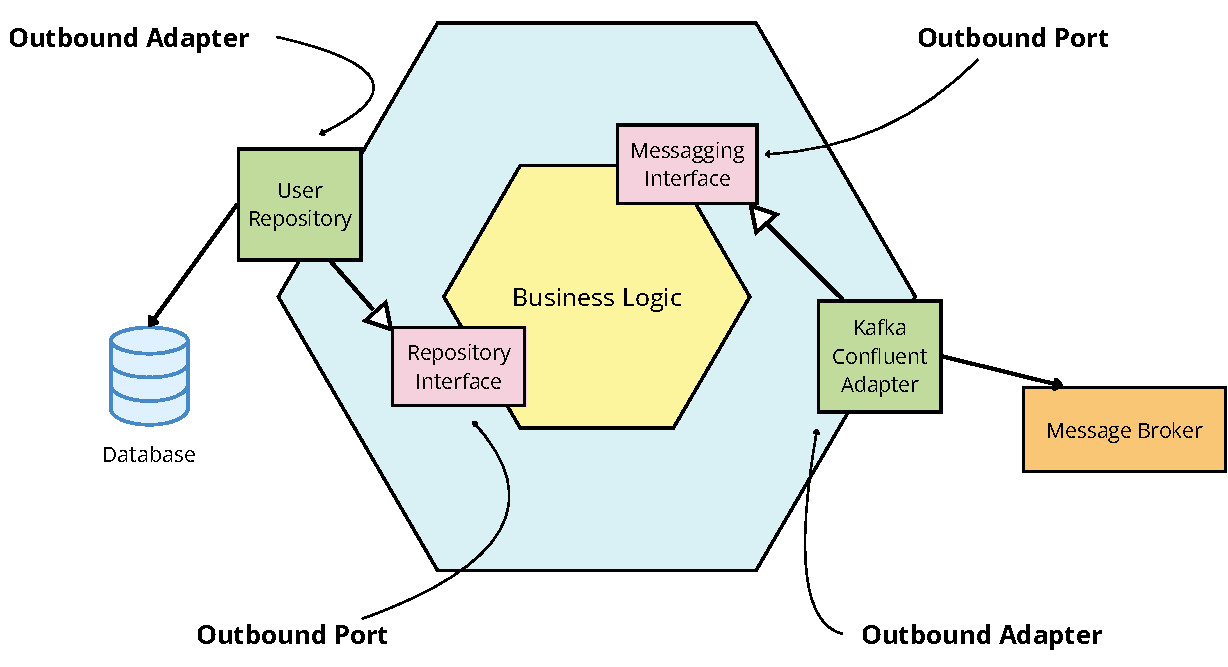
\includegraphics[width=\textwidth]{SimulationService.pdf}
        \caption{Architettura esagonale del SimulationService}
        \end{figure}
        \begin{itemize}
            \item[.] \textbf{Core domain}: Implementa la logica di simulazione del movimento di utenti nello spazio, sfruttando percorsi reali e dinamiche di movimento implementate da diverse strategie. Nella logica di business troviamo infatti il modo in cui avviene la creazione dei vari sensori nel sistema in \texttt{SensorFactory} e il modo in cui vengono simulate le posizioni dei sensori in \texttt{IPositionSimulationStrategy};
            \item[.] \textbf{Inbound ports}: Non dispone di inbound ports in quanto il modulo si occupa della mera creazione di dati fittizi;
            \item[.] \textbf{Outbound ports}: È necessario che il modulo si interfacci con l'esterno: con il database, per garantire una corretta associazione Sensore Simulato - Utente nel sistema, e con un'interfaccia di messaggistica, per pubblicare i dati prodotti dalla logica di business. Nel nostro sistema, le interfacce sono \texttt{IUserRepository}, \texttt{ISensorRepository} e la classe astratta \texttt{PositionSender};
            \sloppy
            \item[.] \textbf{Adapters}: Implementa adattatori come \texttt{ClickhouseUserRepository} e \texttt{ClickhouseSensorRepository} che implementano le rispettive porte e permettono di eseguire le operazioni di accesso al database. Per quanto riguarda la scrittura dei messaggi, l'adapter associato è \texttt{KafkaConfluentAdapter} che sfrutta la tecnologia di message brokering scelta \ref{subsec:Kafka}.
        \end{itemize}

        \item[-] \textbf{Elaboratore di posizioni / Generatore di messaggi}:
        \begin{figure}[H]
        \centering
        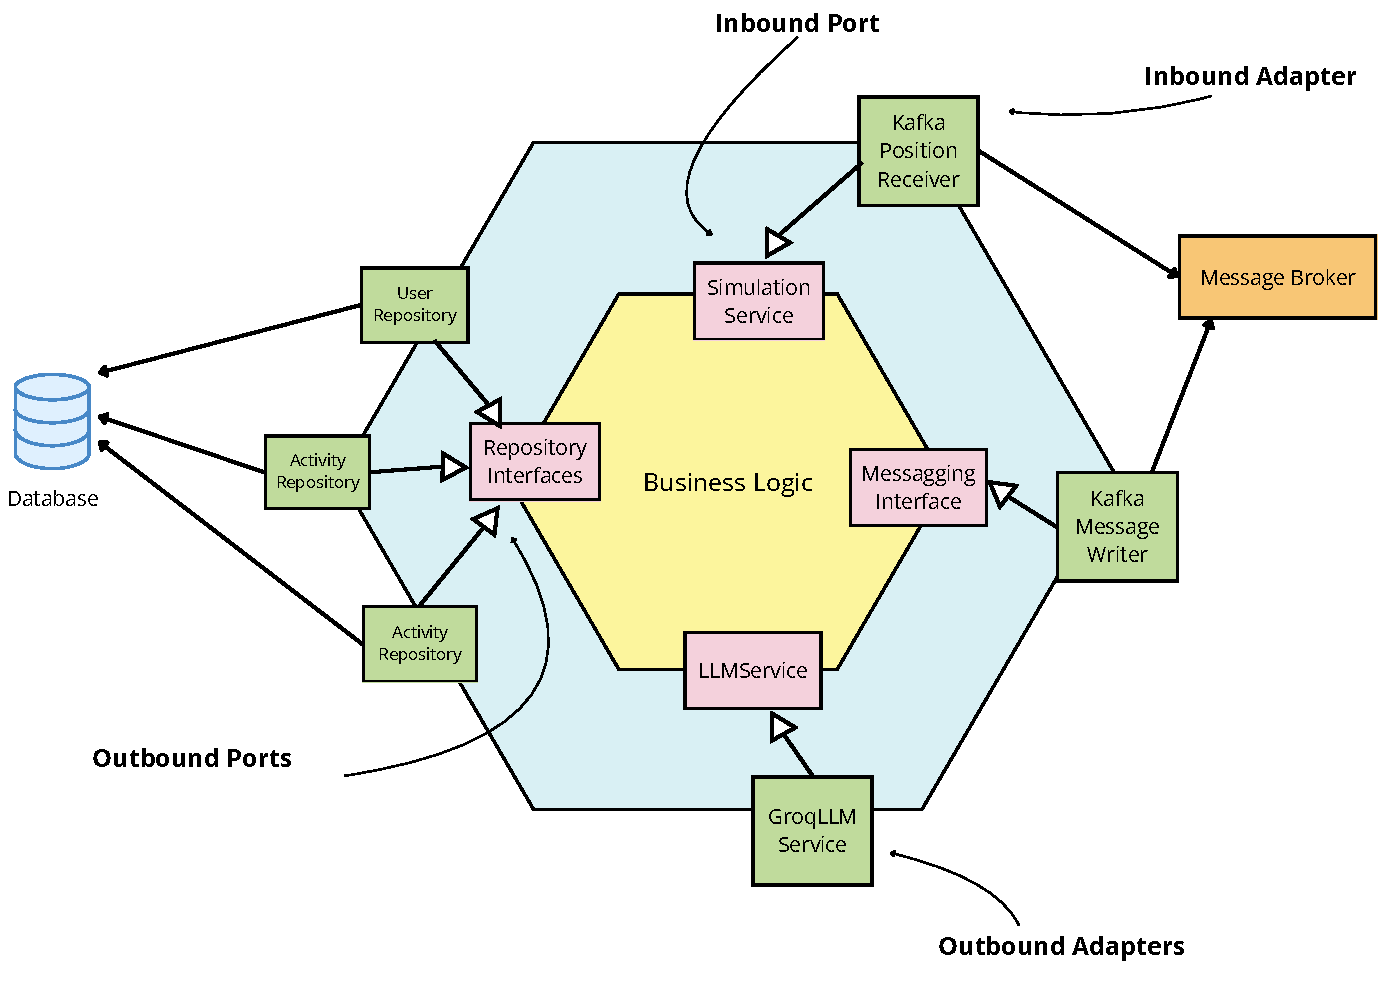
\includegraphics[width=\textwidth]{ProcessorService.pdf}
        \caption{Architettura esagonale del PositionToMessageService}
        \end{figure}
        \begin{itemize}
            \item[.] \textbf{Core domain}: Contiene la logica di identificazione della prossimità e generazione di messaggi pubblicitari. Questa logica permette di elaborare i dati ricevuti tramite la inbound port e tramite il sistema di stream processing \ref{subsec:Flink} , consumandoli come datastream per poi effettuare operazioni di Filter e Mapping su di essi;
            \item[.] \textbf{Inbound ports}: Permette di ricevere i dati che andranno poi elaborati, interfaccia chiamata \texttt{IPositionReceiver};
            \item[.] \textbf{Outbound ports}: Comprende interfacce verso i diversi repository necessari alla logica \\ (\texttt{IUserRepository}, \texttt{IActivityRepository},\texttt{IMessageRepository}), servizi esterni necessari per l'elaborazione dei dati come  (\texttt{LLMService}) e publisher di messaggi (\texttt{IMessageWriter});
            \item[.] \textbf{Adapters}: Implementa adattatori per tecnologie specifiche, come \texttt{KafkaPositionReceiver}, \texttt{ClickHouseActivityAdapter} e \texttt{GroqLLMAdapter}.
        \end{itemize}
    \end{itemize}

    Questo approccio garantisce che ogni componente abbia responsabilità chiaramente definite e che il nucleo di business rimanga indipendente dalle tecnologie utilizzate per l'implementazione.

    % \subsection{Dataflow}

    % \begin{figure}[H]
    %     \centering
    %     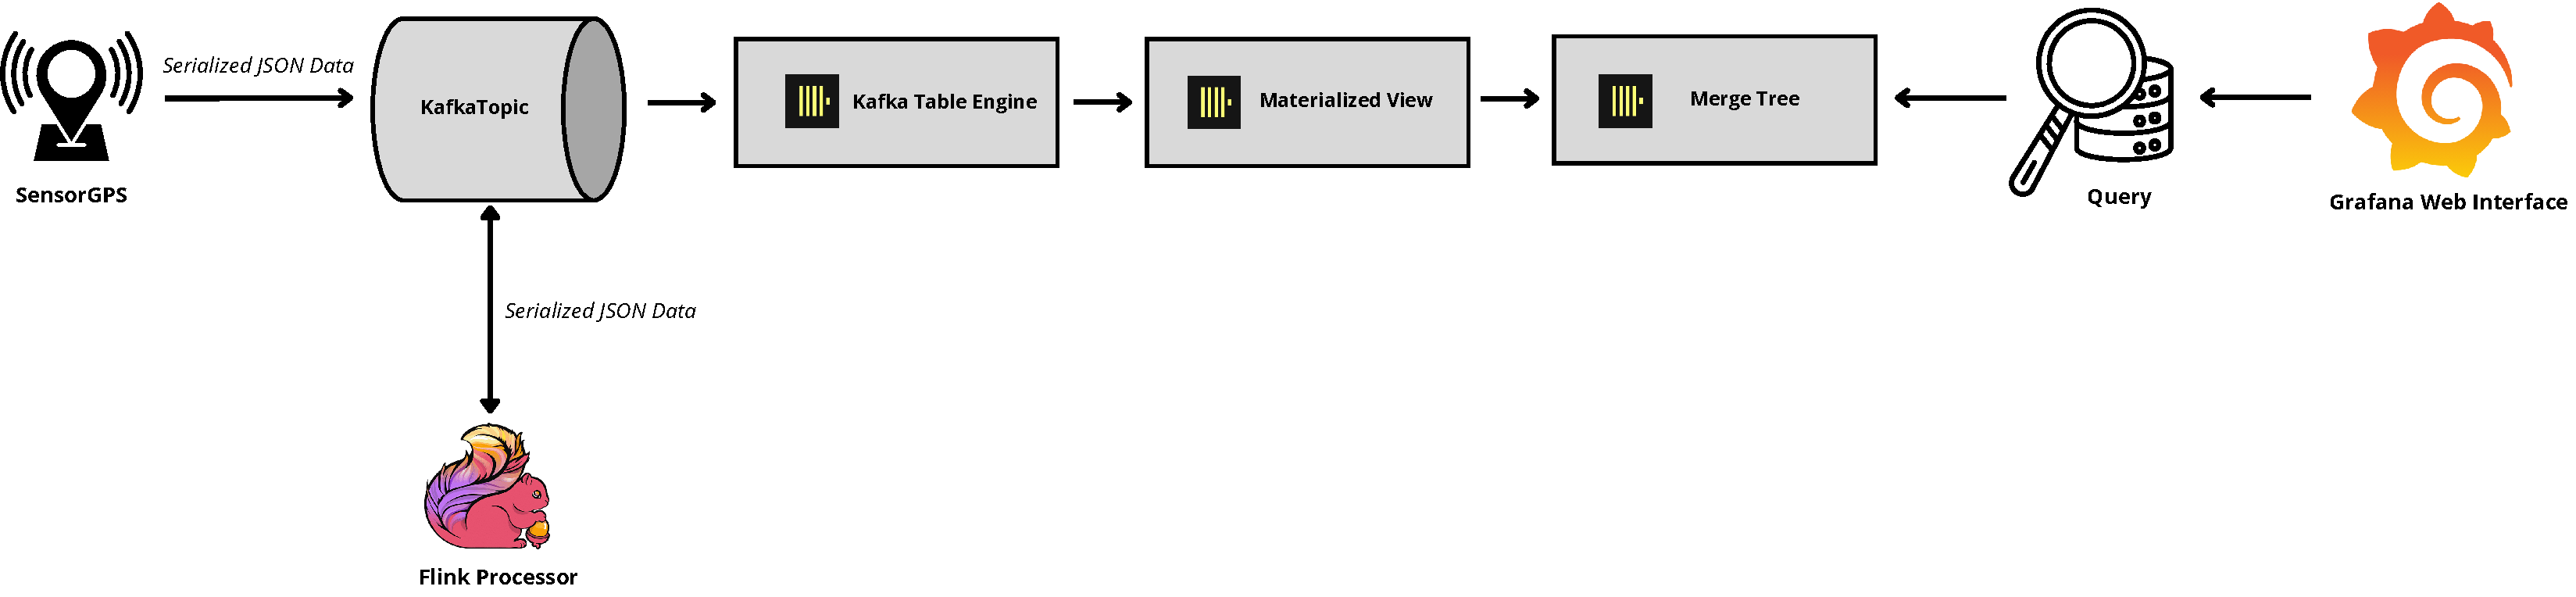
\includegraphics[width=\textwidth]{Dataflow.pdf}
    %     \caption{Flusso dei dati nell'architettura}
    % \end{figure}
    % Il flusso dei dati nell'architetturra di sistema segue un percorso ben definito, garantendo la separazione tra la logica di business e le tecnologie di implementazione. Di seguito viene descritto il flusso di dati end-to-end:
    

    % \begin{enumerate}
    %     \item \textbf{Generazione delle posizioni}:
    %     \begin{itemize}
    %         \item[.] Il core domain del \textit{SimulationService} crea oggetti \texttt{GeoPosition} che rappresentano le coordinate degli utenti;
    %         \item[.] Questi oggetti vengono inviati all'esterno attraverso l'outbound port \texttt{PositionSender};
    %         \item[.] L'adapter \texttt{KafkaConfluentAdapter} serializza i dati in formato JSON e  costruisce un istanza di un Producer che pubblicherà i dati sul topic Kafka \texttt{SimulatorPosition}.
    %     \end{itemize}

    %     \item \textbf{Consumo delle posizioni}:
    %     \begin{itemize}
    %         \item[.] L'inbound adapter \texttt{KafkaPositionReceiver} del servizio \textit{PositionToMessageService} istanzia una \textit{KafkaSource} collegata al topic Kafka \texttt{SimulatorPosition};
    %         \item[.] I payload ricevuti vengono deserializzati secondo uno schema benn definito in \texttt{JsonRowDeserializationSchema} e convertiti in oggetti di dominio \texttt{UserPosition};
    %         \item[.] L'istanza che implementa \texttt{IPositionReceiver} viene collegata al datastream nella logica di business del servizio di elaborazione che elaborerà le posizioni ricevute in input.
    %     \end{itemize}

    %     \item \textbf{Elaborazione e generazione di messaggi}:
    %     \begin{itemize}
    %         \item[.] Il core domain applica una funzione di \textit{Filter},con la classe \texttt{FilterMessageValidator}, al datastream in input per validare i dati ricevuti in input e limitare il \textit{KafkaPoisoning} (scelta esplicata in \ref{poison})
    %         \item[.] Il core domain valuta la prossimità dell'utente rispetto ai punti di interesse, utilizzando l'outbound port \texttt{IUserRepository} per ottenere le informazioni specifiche dell'utente collegato alla posizione ricevuta in input ,utilizza poi \texttt{IActivityRepository} per recuperare le attività nelle vicinanze dell'utente e con gli interessi condivisi;
    %         \item[.] In caso di rilevamento di un punto di interesse valido in prossimità,il core domain \\\texttt{PositionToMessageProcessor} crea un prompt per poi richiedere un messaggio personalizzato tramite l'outbound port \texttt{LLMService};
    %         \item[.] L'adapter \texttt{GroqLLMService} comunica con il servizio LLM esterno e restituisce il messaggio generato;
    %         \item[.] Viene applicata un 'altra funzione di \textit{Filter}, implementata in \texttt{FilterMessageAlreadyDisplayed}, per prevenire la duplicazione di messaggi generati per il singolo utente, necessario per rispettare i requisiti stabiliti. 
    %         \item[.] Il messaggio personalizzato viene incapsulato in un oggetto \texttt{MessageDTO} del dominio per facilitarne la serializzazione.
    %     \end{itemize}

    %     \item \textbf{Pubblicazione del messaggio pubblicitario}:
    %     \begin{itemize}
    %         \item[.] L'oggetto \texttt{MessageDTO} viene passato all'outbound port \texttt{IMessageWriter};
    %         \item[.] L'adapter \texttt{KafkaMessageWriter} serializza il messaggio secondo uno schema ben definito in \\ \texttt{JsonRowSerializationSchema} e lo pubblica sul topic Kafka \texttt{MessageElaborated}.
    %     \end{itemize}

    %     \item \textbf{Persistenza e visualizzazione}:
    %     \begin{itemize}
    %         \item[.] ClickHouse, attraverso il connettore Kafka nativo,in particolare sfruttando le tecnologie \textit{Kafka Table Engine} $\Rightarrow$ \textit{Materialized View} $\Rightarrow$ \textit{Merge Tree} consuma e archivia nella apposita tabella i messaggi dal topic \texttt{messageTable};
    %         \item[.] Grafana interroga ClickHouse tramite l'apposito plugin e il sistema di query, per recuperare e visualizzare i dati in tempo reale attraverso dashboard interattive.
    %     \end{itemize}
    % \end{enumerate}

    % Il flusso dei dati è progettato per essere asincrono, garantendo la scalabilità e la resilienza del sistema. Ogni componente può funzionare indipendentemente, con Kafka che funge da buffer di messaggi affidabile tra i vari stadi del processo.

    % Gli adattatori si occupano d'interfacciarsi con l'esterno: il simulatore di posizioni produce eventi JSON su Kafka, successivamente elaborati da Flink per definire la prossimità ai punti di interesse e gestire i dati necessari alla logica di dominio. Qualora sia richiesta la generazione di contenuti, un LLM esterno crea i messaggi personalizzati che confluiscono nel dominio. La persistenza e la consultazione storica avvengono tramite ClickHouse, mentre Grafana rende immediatamente disponibili tali informazioni agli utenti.

    % Questo utilizzo di Kafka come backbone di comunicazione sostiene la natura asincrona ed event-driven del sistema, svincolando i componenti gli uni dagli altri. Grazie a questa separazione in porte e adattatori, l'architettura risulta flessibile, manutenibile e facile da testare: ogni modifica alla periferia può essere gestita senza impattare la logica di dominio, preservando nel contempo la coerenza e la semplicità di estensione all'intero sistema.

\newpage
%SPOSTATA SOTTO
% \section{Integrazione Architettura logica e Architettura di sistema}
% \subsection{Descrizione}
% Le due architetture, la Kappa Architecture e l'architettura esagonale, rappresentano due prospettive differenti dello stesso sistema.
% Mentre la Kappa Architecture si riferisce all’implementazione concreta del codice e al flusso continuodi dati in tempo reale, l’architettura esagonale evidenzia la separazione logicatra il core di business e le interfacce esterne.
% Nonostante l'approccio e la terminologia differiscano, i componenti  del sistema sono gli stessi condivisi fra le due architetture e possono quindi essere mappati fra di loro.
% Ovviamente, il layer di Visualizzazione non rientra nell'architettura esagonale, poiché non è un componente realizzato dal gruppo, ma si interfaccia solamente con il database ClickHouse per la parte di interfaccia utente.
% \subsection{Mappatura dei componenti}

% \begin{table}[H]
% \centering
% \renewcommand{\arraystretch}{1.5}
% \rowcolors{0}{gray!11}{white}
% \begin{tabular}{|>{\centering\arraybackslash}m{4cm}|>{\centering\arraybackslash}m{4cm}|>{\raggedright\arraybackslash}m{6cm}|}
% \hline
% \rowcolor{gray!25}
% \textbf{Kappa Architecture} & \textbf{Architettura Esagonale} & \textbf{Ruolo nel Progetto} \\
% \hline
% Log Immutabile & \textit{SimulationService} Outbound Port & Il servizio che si occupa di creare posizioni simulate , invia queste ultime tramite l'apposita outbound port, come uno stream di dati persistente, partizionato per utente e ordinato temporalmente, implementato con ApacheKafka, usando il topic\texttt{SimulatorPosition}. \\
% \hline
% Stream Processing Engine & \textit{PositionToMessageService} Inbound Port/Core Logic & Il servizio riceve le posizioni tramite l'apposita Inbound Port, elabora lo stream in tempo reale e parallelamente al numero di utenti , trasformando lo stream\\
% \hline
% Viste Materializzate & \textit{PositionToMessageService} Outbound Port & Si occupa di prelevare i dati dello stream elaborato e storicizzarlo nell'apposito database clickhouse ottimizzato per rispondere alle query dell0interfaccia grafica in maniera efficiente \\
% \hline
% \end{tabular}
% \caption{Mappatura dei componenti tra Kappa Architecture e Architettura Esagonale}
% \label{tab:mappatura_componenti}
% \end{table}

\newpage
\section{Architettura del Sistema}

\subsection{Panoramica architetturale}
L'architettura del progetto si basa su un insieme di microservizi event-driven che comunicano fra di loro mediante Kafka. I dati di posizione vengono raccolti in tempo reale, elaborati per verificare la prossimità dei punti d'interesse ed eventualmente sottoporli ad un servizio LLM che genera messaggi pubblicitari personalizzati per l'utente in base al tipo della attività.

\subsection{K-Architecture: Event Streaming Platform}
La Kappa Architecture è stata selezionata come architettura di riferimento per il progetto in virtù della sua capacità di unificare l’elaborazione di dati in tempo reale e batch all’interno di un unico stack tecnologico, garantendo flessibilità, semplicità operativa e scalabilità. Il vantaggio principale è l’eliminazione della duplicazione di tecnologie e pipeline tipica della Lambda Architecture. In quest’ultima, due sistemi separati (uno per il batch e uno per lo streaming) richiedono codice, logiche e infrastrutture distinte, aumentando i costi di sviluppo,
    \subsubsection{Motivazioni della scelta architetturale}
        \begin{itemize}
        \item \textbf{Vantaggi per l'elaborazione in tempo reale}: Tra i vantaggi per l'elaborazione in tempo reale c'è la capacità di gestire flussi di dati continui senza ritardi significativi.
        \item \textbf{Tecniche di riduzione della latenza}: La riduzione della latenza è garantita dalla gestione dei dati in tempo reale, senza la necessità di processi batch.
        \item \textbf{Benefici sul disaccoppiamento}: Tra i benefici sul disaccoppiamento c'è la possibilità di sviluppare e scalare indipendentemente i componenti del sistema, garantendo una maggiore flessibilità.
        \item \textbf{Ottimizzazione del codebase}: La semplificazione della pipeline di dati permette di ridurre la complessità del codice e di semplificare la manutenzione.
    \end{itemize}

\subsubsection{Componenti principali}
Il progetto si suddivide in cinque componenti principali, ognuno dei quali svolge un ruolo specifico nell'architettura complessiva:
\begin{itemize}
    \item[-] Data Source;
    \item[-] Straming Layer;
    \item[-] Processing Layer;
    \item[-] Storage Layer;
    \item[-] Data Visualization.
\end{itemize}

\begin{figure}[H]
    \centering
    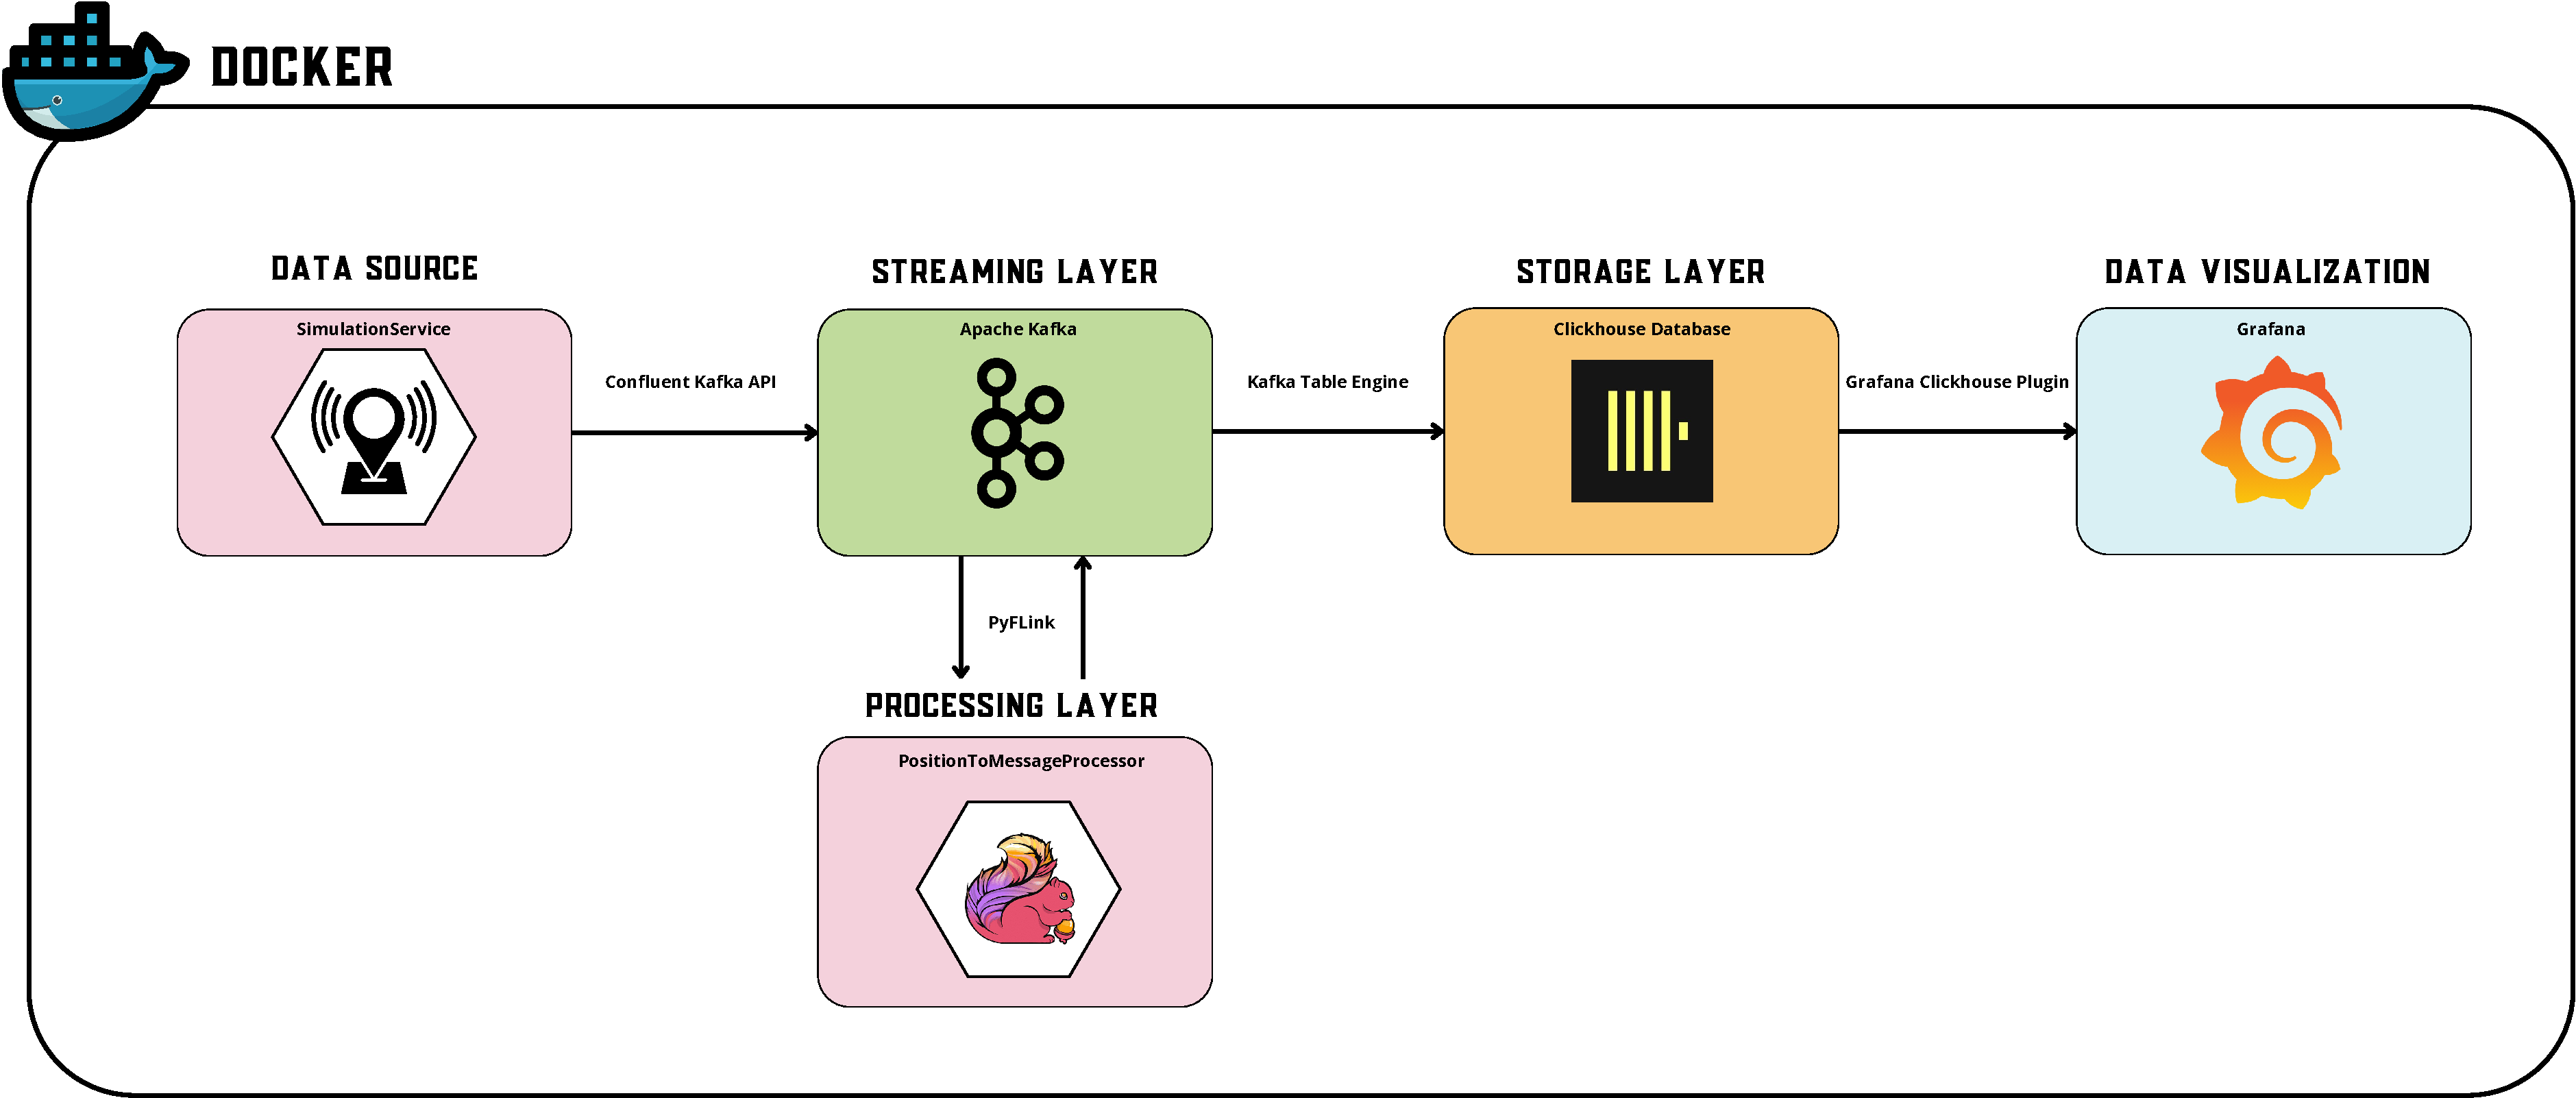
\includegraphics[width=\textwidth]{SystemArchitecture.pdf}
    \caption{Diagramma dell'architettura di Sistema}
\end{figure}

Descrizione dei componenti dell'architettura:
\begin{itemize}
    \item \textbf{Data Source}: Il ruolo di questo componente è coperto dal \textit{SimulationService}, che si occupa della generazione delle posizioni appartenenti a percorsi realisti.
    \item \textbf{Streaming Layer}: Basato su Apache Kafka, gestisce la comunicazione asincrona tra i microservizi, garantendo la scalabilità e la resilienza del sistema grazie alla gestione dei topic e delle partizioni con le chiavi che corrispondono all'id del sensore per facilitare l'elaborazione in maniera parallela. Infine Kafka è responsabile della storicizzazione dei log nelle apposite entry del database ClickHouse.
    \item \textbf{Elaborazione dei dati}: Implementato con il \textit{PositionToMessageService} che sfrutta le funzionalità Apache Flink, elabora i dati valutando la prossimità dei punti d’interesse e interagendo con l’LLM per generare annunci personalizzati.
    \item \textbf{Storage}: Supportato dal database ClickHouse, memorizza i dati in tabelle colonnari ad alte prestazioni, consentendo query analitiche rapide grazie all’ottimizzazione per letture intensive.
    \item \textbf{Visualizzazione}: Basato su Grafana, costituisce una soluzione di visualizzazione dei dati su una mappa e l'integrazione di tale interfaccia con i dati del datasource avviene tramite delle query. Sfrutta inoltre il connettore nativo di ClickHouse, permettendo l'integrazione e le query in tempo reale delle informazioni.
\end{itemize}




\subsection{Integrazione Architettura logica e Architettura di sistema}
\subsubsection{Descrizione}
Le due architetture, la Kappa Architecture e l'architettura esagonale, rappresentano due prospettive differenti dello stesso sistema.
Mentre la Kappa Architecture si riferisce all’implementazione concreta del codice e al flusso continuo di dati in tempo reale, l’architettura esagonale evidenzia la separazione logica tra il core di business e le interfacce esterne.
Nonostante l'approccio e la terminologia differiscano, i componenti  del sistema sono gli stessi condivisi fra le due architetture e possono quindi essere mappati fra di loro.
Ovviamente, il layer di Visualizzazione non rientra nell'architettura esagonale, poiché non è un componente realizzato dal gruppo, ma si interfaccia solamente con il database ClickHouse per la parte di interfaccia utente.
\subsubsection{Mappatura dei componenti}

\begin{table}[H]
\centering
\renewcommand{\arraystretch}{1.5}
\rowcolors{0}{gray!11}{white}
\begin{tabular}{|>{\centering\arraybackslash}m{4cm}|>{\centering\arraybackslash}m{4cm}|>{\raggedright\arraybackslash}m{6cm}|}
\hline
\rowcolor{gray!25}
\textbf{Kappa Architecture} & \textbf{Architettura Esagonale} & \textbf{Ruolo nel Progetto} \\
\hline
Log Immutabile & \textit{SimulationService} Outbound Port & Il servizio che si occupa di creare le posizioni simulate, invia queste ultime tramite l'apposita outbound port, come uno stream di dati persistente, partizionato per utente e ordinato temporalmente, implementato con ApacheKafka, usando il topic \texttt{SimulatorPosition}. \\
\hline
Stream Processing Engine & \textit{PositionToMessageService} Inbound Port/Core Logic & Il servizio riceve le posizioni tramite l'apposita Inbound Port, elabora lo stream in tempo reale, parallelamente per ogni singolo utente\\
\hline
Viste Materializzate & \textit{PositionToMessageService} Outbound Port & Si occupa di prelevare i dati dello stream elaborato e storicizzarli nell'apposito database ClickHouse ottimizzato per rispondere alle query dell'interfaccia grafica in maniera efficiente\\
\hline
\end{tabular}
\caption{Mappatura dei componenti tra Kappa Architecture e Architettura Esagonale}
\label{tab:mappatura_componenti}
\end{table}



    \subsection{Dataflow}

    \begin{figure}[H]
        \centering
        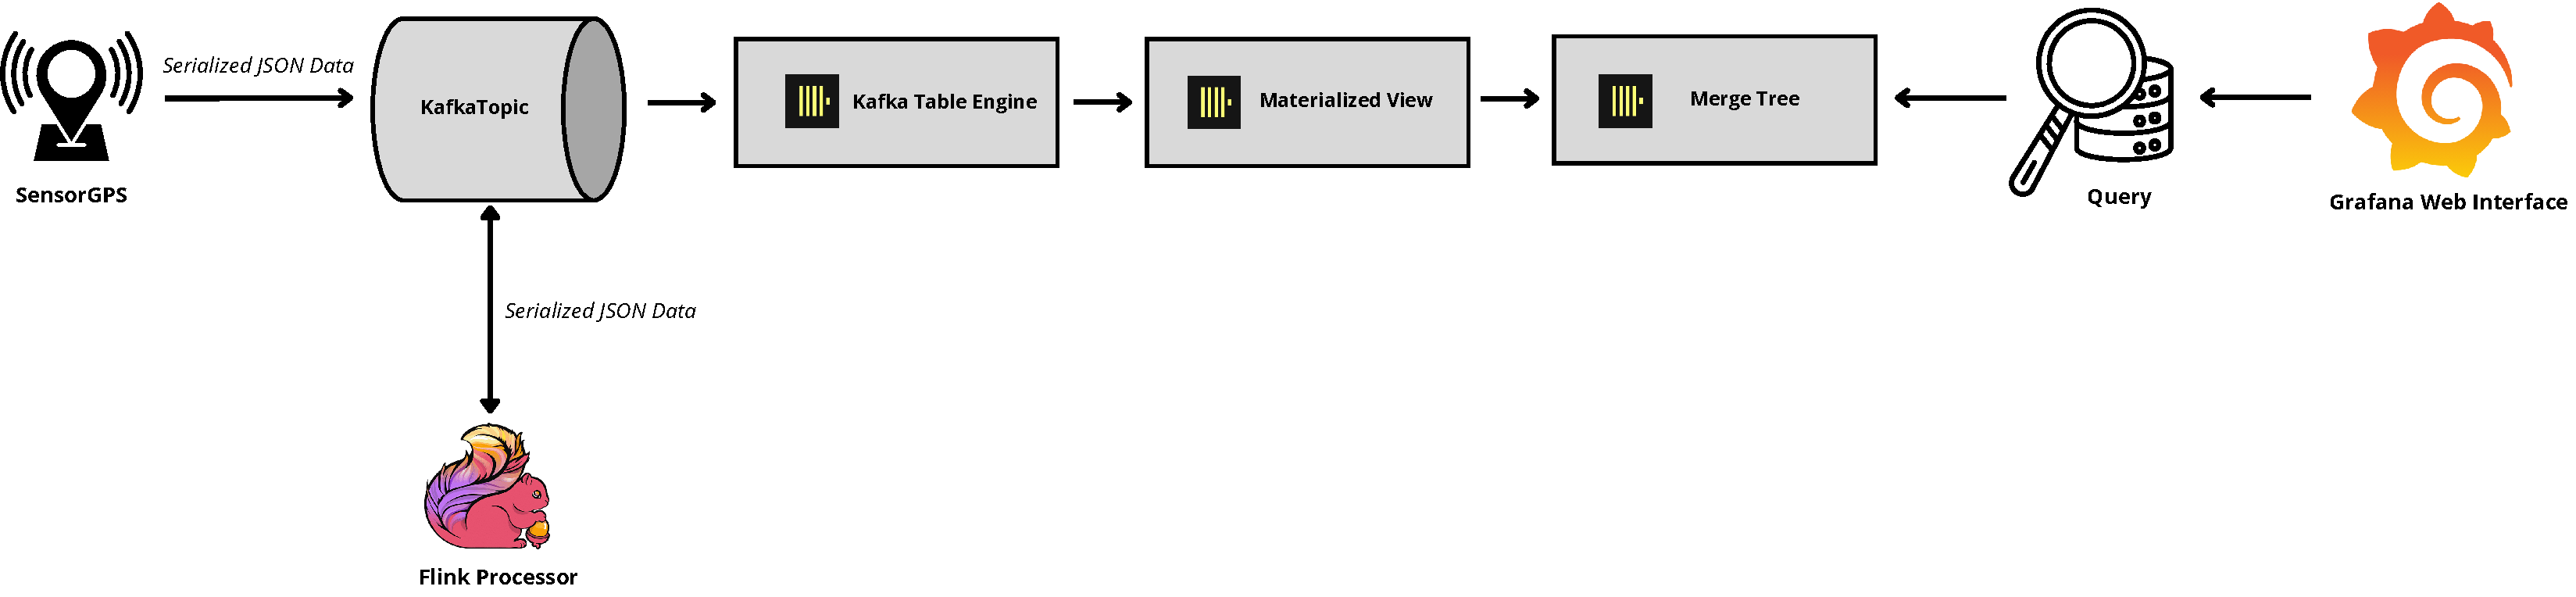
\includegraphics[width=\textwidth]{Dataflow.pdf}
        \caption{Flusso dei dati nell'architettura}
    \end{figure}
    Il flusso dei dati nell'architetturra di sistema segue un percorso ben definito, garantendo la separazione tra la logica di business e le tecnologie di implementazione. Di seguito viene descritto il flusso di dati end-to-end:
    

    \begin{enumerate}
        \item \textbf{Generazione delle posizioni}:
        \begin{itemize}
            \item[.] Il core domain del \textit{SimulationService} crea oggetti \texttt{GeoPosition} che rappresentano le coordinate degli utenti;
            \item[.] Questi oggetti vengono inviati all'esterno attraverso l'outbound port \texttt{PositionSender};
            \item[.] L'adapter \texttt{KafkaConfluentAdapter} serializza i dati in formato JSON e  costruisce un istanza di un Producer che pubblicherà i dati sul topic Kafka \texttt{SimulatorPosition}.
        \end{itemize}

        \item \textbf{Consumo delle posizioni}:
        \begin{itemize}
            \item[.] L'inbound adapter \texttt{KafkaPositionReceiver} del servizio \textit{PositionToMessageService} istanzia una \textit{KafkaSource} collegata al topic Kafka \texttt{SimulatorPosition};
            \item[.] I payload ricevuti vengono deserializzati secondo uno schema ben definito in \\ \texttt{JsonRowDeserializationSchema} e convertiti in oggetti di dominio \texttt{UserPosition};
            \item[.] L'istanza che implementa \texttt{IPositionReceiver} viene collegata al datastream nella logica di business del servizio di elaborazione che elaborerà le posizioni ricevute in input.
        \end{itemize}

        \item \textbf{Elaborazione e generazione di messaggi}:
        \begin{itemize}
            \item[.] Il core domain applica una funzione di \textit{Filter}, con la classe \texttt{FilterMessageValidator}, al datastream in input per validare i dati ricevuti in input e limitare il \textit{KafkaPoisoning} (scelta esplicata in \ref{poison})
            \item[.] Il core domain valuta la prossimità dell'utente rispetto ai punti di interesse, utilizzando l'outbound port \texttt{IUserRepository} per ottenere le informazioni specifiche dell'utente collegato alla posizione ricevuta in input, utilizza poi \texttt{IActivityRepository} per recuperare le attività nelle vicinanze dell'utente e con gli interessi condivisi;
            \item[.] In caso di rilevamento di un punto di interesse valido in prossimità, il core domain \\\texttt{PositionToMessageProcessor} crea un prompt per poi richiedere un messaggio personalizzato tramite l'outbound port \texttt{LLMService};
            \item[.] L'adapter \texttt{GroqLLMService} comunica con il servizio LLM esterno e restituisce il messaggio generato;
            \item[.] Viene applicata un'altra funzione di \textit{Filter}, implementata in \texttt{FilterMessageAlreadyDisplayed}, per prevenire la duplicazione di messaggi generati per il singolo utente, necessario per rispettare i requisiti stabiliti. 
            \item[.] Il messaggio personalizzato viene incapsulato in un oggetto \texttt{MessageDTO} del dominio per facilitarne la serializzazione.
        \end{itemize}

        \item \textbf{Pubblicazione del messaggio pubblicitario}:
        \begin{itemize}
            \item[.] L'oggetto \texttt{MessageDTO} viene passato all'outbound port \texttt{IMessageWriter};
            \item[.] L'adapter \texttt{KafkaMessageWriter} serializza il messaggio secondo uno schema ben definito in \\ \texttt{JsonRowSerializationSchema} e lo pubblica sul topic Kafka \texttt{MessageElaborated}.
        \end{itemize}

        \item \textbf{Persistenza e visualizzazione}:
        \begin{itemize}
            \item[.] ClickHouse, attraverso il connettore Kafka nativo, in particolare sfruttando le tecnologie \textit{Kafka Table Engine} $\Rightarrow$ \textit{Materialized View} $\Rightarrow$ \textit{Merge Tree} consuma e archivia nella apposita tabella i messaggi dal topic \texttt{messageTable};
            \item[.] Grafana interroga ClickHouse tramite l'apposito plugin e il sistema di query, per recuperare e visualizzare i dati in tempo reale attraverso dashboard interattive.
        \end{itemize}
    \end{enumerate}

    Il flusso dei dati è progettato per essere asincrono, garantendo la scalabilità e la resilienza del sistema. Ogni componente può funzionare indipendentemente, con Kafka che funge da buffer di messaggi affidabile tra i vari stadi del processo.

    Gli adattatori si occupano d'interfacciarsi con l'esterno: il simulatore di posizioni produce eventi JSON su Kafka, successivamente elaborati da Flink per definire la prossimità ai punti di interesse e gestire i dati necessari alla logica di dominio. Qualora sia richiesta la generazione di contenuti, un LLM esterno crea i messaggi personalizzati che confluiscono nel dominio. La persistenza e la consultazione storica avvengono tramite ClickHouse, mentre Grafana rende immediatamente disponibili tali informazioni agli utenti.

    Questo utilizzo di Kafka come backbone di comunicazione sostiene la natura asincrona ed event-driven del sistema, svincolando i componenti gli uni dagli altri. Grazie a questa separazione in porte e adattatori, l'architettura risulta flessibile, manutenibile e facile da testare: ogni modifica alla periferia può essere gestita senza impattare la logica di dominio, preservando nel contempo la coerenza e la semplicità di estensione all'intero sistema.
% \subsubsection{Flusso di dati end-to-end}
% \begin{enumerate}
%     \item Il simulatore genera dati di posizione e li invia a Kafka, includendo informazioni sul timestamp e sull’ID sensore.
%     \item Flink legge i topic, rileva la prossimità dei punti d’interesse tramite ClickHouse e genera un messaggio tramite l'LLM passandogli le informazioni.
%     \item L’LLM elabora i dati che gli vengono passati, producendo un messaggio personalizzato ad esempio in base al tipo di attività, poi viene prodotto il messaggio, pubblicato su Kafka e di conseguenza su ClickHouse.
%     \item Grafana interroga ClickHouse e preleva i dati per la visualizzazione in tempo reale tramite dashboard di attività, utenti, relative posizioni e annunci generati.
% \end{enumerate}

% \subsubsection{Interfacce tra componenti}
%%TODO: questo forse è ridondate quindi è da controllare
%% Le comunicazioni tra componenti avvengono su Kafka, con dati strutturati in formato JSON. Per quanto riguarda l'integrazione fra Kafka e ClickHouse è presente un connettore nativo che permette inoltre di creare delle materialized view per la storicizzazione dei dati. Per Grafana è sempre presente un connettore nativo per ClickHouse che permette di interrogare il database e visualizzare i dati in tempo reale.

    \subsection{Implementazione tecnica dei componenti principali}
        \subsubsection{DataSource - Simulation Service}
        Il SimulationModule è una componente architettonica progettata per simulare dati di posizionamento geografico in un ecosistema più ampio di gestione dati. Questo modulo rappresenta l'applicazione pratica dell'integrazione tra i principi della Kappa Architecture e dell'Architettura Esagonale.

        
        Il sistema opera attraverso tre fasi fondamentali. Inizialmente, prepara l'ambiente di simulazione acquisendo le risorse necessarie e configurando il modello geografico. In questa parte vengono creati i sensori che sono associati uno ad uno con gli utenti gia registrati nel sistema. Successivamente, viene attivato il processo di simulazione che genera flussi di dati rappresentanti movimenti virtuali attraverso percorsi realistici. Infine, questi dati vengono incanalati verso il sistema di streaming centrale.

        La simulazione crea un flusso continuo di eventi che rispecchia scenari di movimento reali. Questo approccio event-driven si allinea perfettamente con la filosofia Kappa, dove tutti i dati sono modellati come flussi di eventi, mentre la struttura interna rispetta i principi dell'Architettura Esagonale.


        % \myparagraph{Simulatore posizioni}
        % Il simulatore di posizioni è un componente fondamentale dell'architettura che simula i dati GPS degli utenti, consentendo di testare e dimostrare il funzionamento del sistema senza richiedere dispositivi fisici reali.

        % \mysubparagraph{Strategie di movimento}
        % Il simulatore implementa il pattern Strategy per definire diverse modalità di movimento. L'interfaccia \texttt{IPositionSimulationStrategy} definisce il contratto comune per tutte le strategie di simulazione:
        % \begin{lstlisting}
        % class IPositionSimulationStrategy(ABC):
        %     @abstractmethod
        %     def simulate_position_live_update(self, sensor_istance):
        %         pass
        % \end{lstlisting}

        % La strategia principale implementata, \texttt{BycicleSimulationStrategy}, simula il movimento di una bicicletta su un grafo stradale reale utilizzando la libreria OSMnx. Questa strategia:
        % \begin{itemize}
        %     \item[-] Seleziona casualmente nodi nel grafo stradale per creare percorsi realistici;
        %     \item[-] Utilizza una velocità parametrizzabile (default: 10-20 km/h);
        %     \item[-] Applica interpolazione lineare tra i punti del percorso;
        %     \item[-] Consente configurazione temporale degli aggiornamenti di posizione.
        % \end{itemize}

        % \mysubparagraph{Generazione dati JSON}
        % La serializzazione dei dati avviene attraverso il pattern Adapter, implementato dalla classe \texttt{PositionJsonAdapter} che converte gli oggetti \texttt{GeoPosition} in formato JSON:
        % \begin{lstlisting}
        % {
        %     "id": "UUID",
        %     "latitude": "Float64",
        %     "longitude": "Float64",
        %     "received_at": "String"
        % }
        % \end{lstlisting}

        % Questo formato è compatibile con le aspettative del topic Kafka \texttt{SimulatorPosition} e della tabella ClickHouse corrispondente. L'adapter implementa l'interfaccia \texttt{IJsonSerializable}, garantendo uniformità nella serializzazione di diversi tipi di dati.

        % \mysubparagraph{Configurazione del simulatore}
        % Il simulatore è altamente configurabile attraverso diversi parametri:
        % \begin{itemize}
        %     \item[-] \textbf{Delta tempo}: Intervallo temporale tra aggiornamenti di posizione;
        %     \item[-] \textbf{Range di velocità}: Valori minimi e massimi per la velocità di spostamento;
        %     \item[-] \textbf{Area geografica}: Delimitazione dell'area in cui generare percorsi;
        %     \item[-] \textbf{Numero di sensori}: Quantità di sensori simulati simultaneamente.
        % \end{itemize}

        % La configurazione sfrutta la libreria OSMnx per caricare grafi stradali reali. Il sistema utilizza un grafo precaricato dell'area di interesse per ottimizzare le performance di avvio:
        % \begin{lstlisting}
        % graph_istance = GraphWrapper().get_graph()
        % strategy_simulation = BycicleSimulationStrategy()
        % sensor_istance = sensor_factory.create_sensor(sensor_uuid, strategy_simulation)
        % \end{lstlisting}

        % \mysubparagraph{Tipologie di dati generati}
        % Il simulatore produce dati con le seguenti caratteristiche:
        % \begin{itemize}
        %     \item[-] \textbf{Continuità spaziale}: I punti generati seguono percorsi realistici lungo le strade del grafo OSM;
        %     \item[-] \textbf{Variabilità temporale}: Gli aggiornamenti rispettano intervalli di tempo configurabili;
        %     \item[-] \textbf{Coerenza di velocità}: La distanza tra punti consecutivi è proporzionale alla velocità simulata.
        % \end{itemize}

        % La classe \texttt{GeoPosition} rappresenta la struttura dati fondamentale per le posizioni:
        % \begin{lstlisting}
        % class GeoPosition:
        %     def __init__(self, sensor_id, latitude, longitude, timestamp):
        %         self.__sensor_id = sensor_id
        %         self.__latitude = latitude
        %         self.__longitude = longitude
        %         self.__timestamp = timestamp
        % \end{lstlisting}
        
        \myparagraph{Diagramma della classi }


        
        \begin{figure}[H]
        \hspace{-1.5cm} % Sposta l'immagine di 2cm a sinistra
        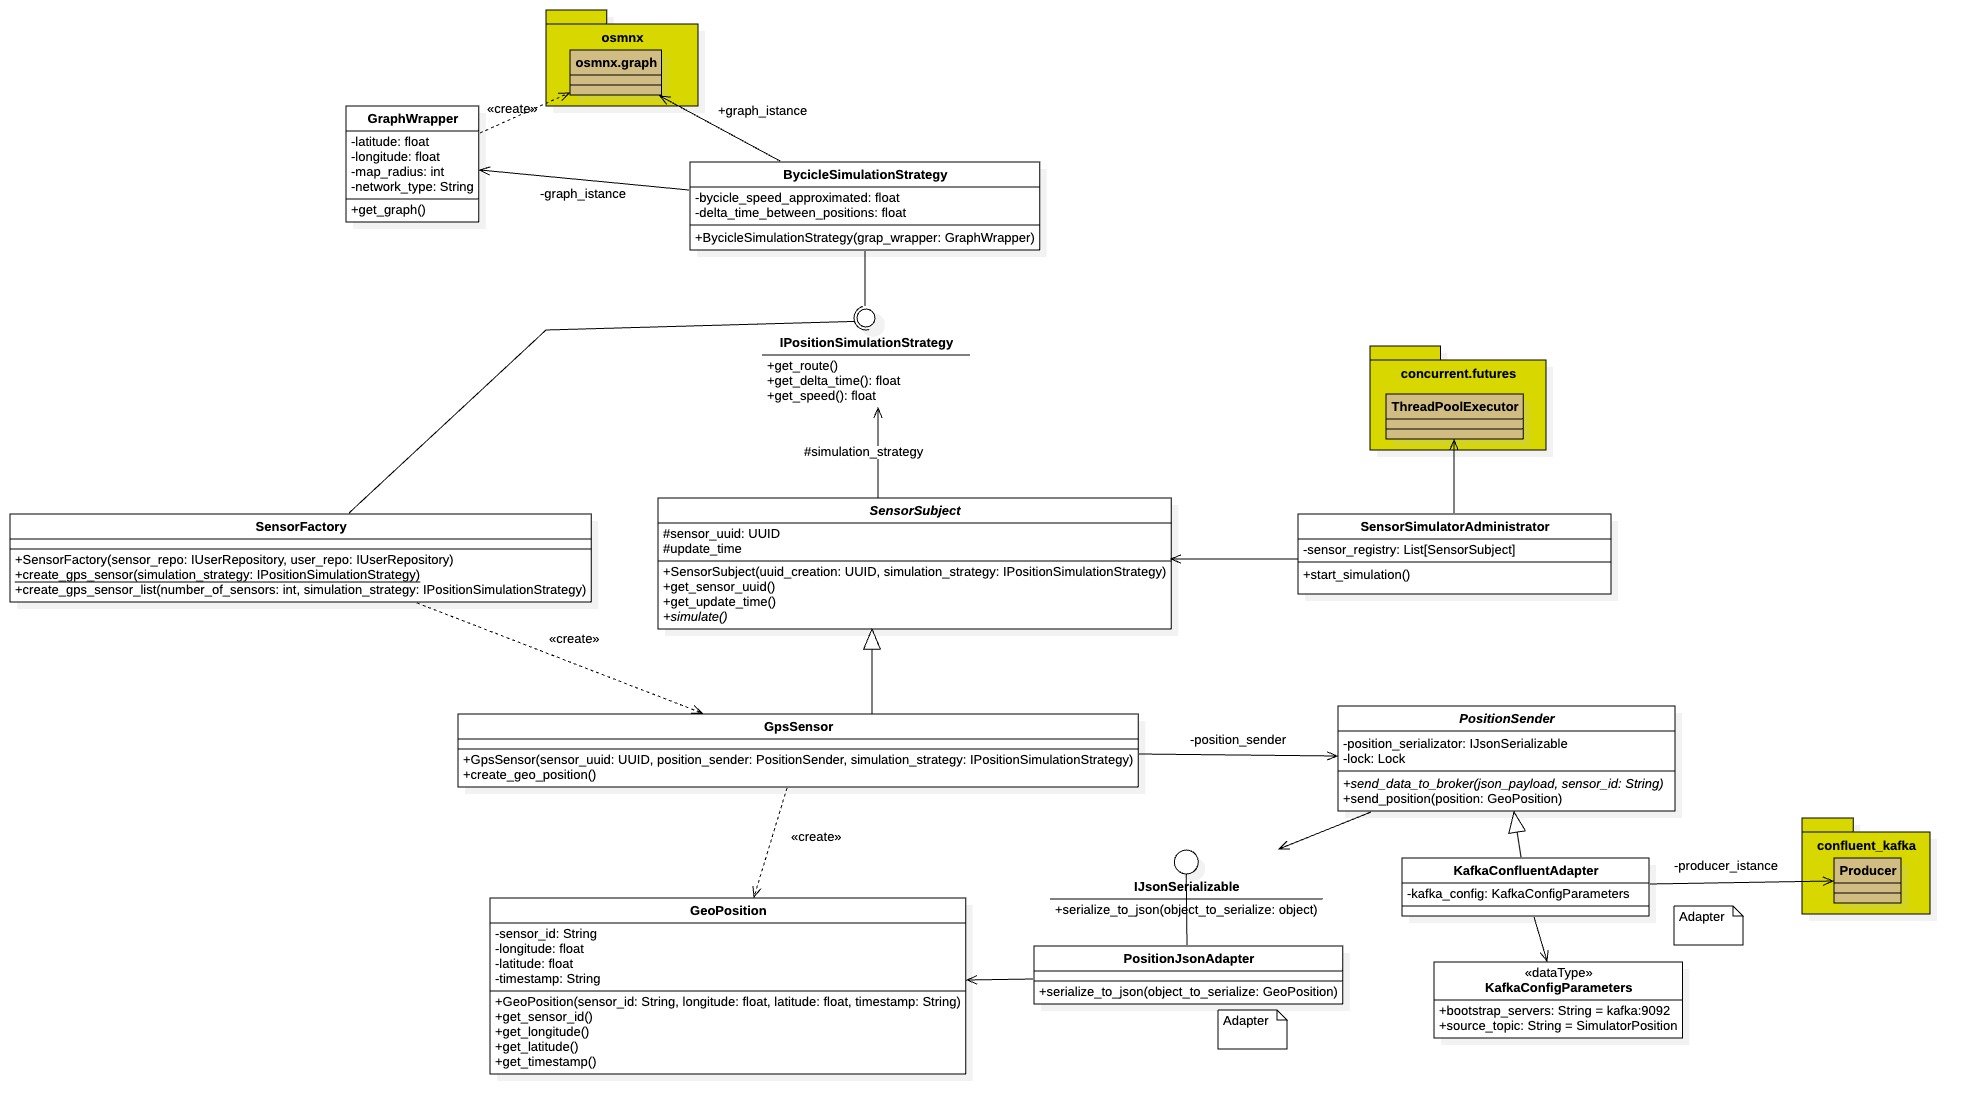
\includegraphics[width=1.24\textwidth]{CoreSimulation.jpg}
        \caption{SimulationService Core}
        \end{figure}

        \begin{figure}[H]
        \hspace{-1.5cm}
        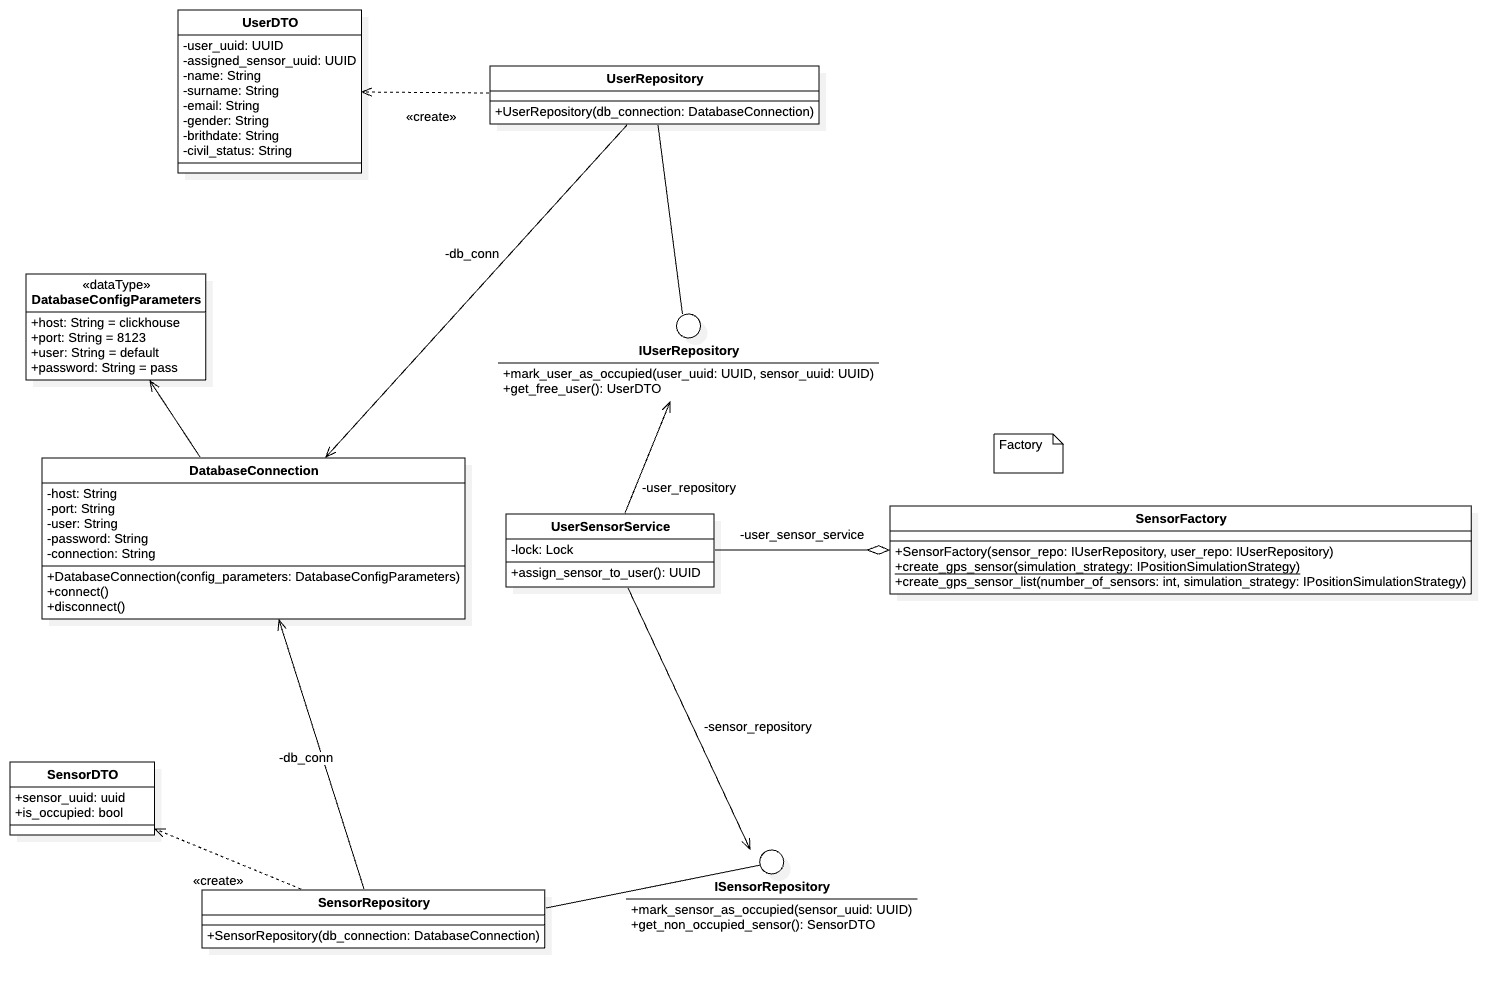
\includegraphics[width=1.25\textwidth]{SensorFactory.jpg}
        \caption{Factory di Sensori}
        \end{figure}


    \myparagraph{Design Pattern - Strategy Pattern}

    \mysubparagraph{Motivazioni e studio del design pattern}
    Il pattern Strategy è stato adottato per incrementare la flessibilità nella gestione di diverse modalità operative del sistema. Questa scelta architetturale permette di definire un'interfaccia comune per tutte le strategie implementate, consentendo di modificare il comportamento del sistema selezionando una strategia specifica. Tale approccio aderisce al principio Open/Closed, agevolando l'aggiunta di nuove strategie senza intervenire su quelle esistenti.

    \mysubparagraph{Implementazione del design pattern}
    Il pattern Strategy è implementato attraverso la definizione di un'interfaccia che delinea il comportamento comune a tutte le strategie. Ogni strategia concreta realizza questa interfaccia, fornendo un'implementazione specifica per una determinata funzionalità. Questo design consente la selezione dinamica della strategia più appropriata in base alle esigenze operative, migliorando la modularità e la manutenibilità del codice complessivo.

    \mysubparagraph{Utilizzo}
    L'integrazione del pattern Strategy disaccoppia la logica specifica delle funzionalità dal codice client che le invoca, semplificando l'estensibilità del sistema. La possibilità di scegliere le strategie a runtime permette di adattare dinamicamente il comportamento dell'applicazione in base al contesto. Ciò si rivela particolarmente vantaggioso in scenari che richiedono la sperimentazione o l'utilizzo di diverse modalità operative senza necessità di modifiche al nucleo del codice.

    \mysubparagraph{Integrazione del pattern}
    Il pattern Strategy si compone di tre elementi principali: un contesto che utilizza la strategia, un'interfaccia che definisce il contratto comune e le classi concrete che implementano le varie strategie. Nel nostro sistema, questo pattern è implementato in diversi modi:
    \begin{itemize}
        \item Per la simulazione della posizione, il nostro sistema utilizza l'interfaccia IPositionSimulationStrategy, un contratto che definisce tre metodi astratti: get\_route(), get\_delta\_time() e get\_speed(). Questa interfaccia, basata sul pattern Strategy, permette di implementare diverse logiche di simulazione, garantendo flessibilità ed estendibilità per vari scenari di utilizzo.
        \begin{lstlisting}
        class IPositionSimulationStrategy(ABC):
            @abstractmethod
            def get_route(self):
                pass

            @abstractmethod
            def get_delta_time(self) -> float:
                pass

            @abstractmethod
            def get_speed(self) -> float:
                pass
        \end{lstlisting}
        La strategia concreta BycicleSimulationStrategy implementa l'interfaccia IPositionSimulationStrategy, fornendo un algoritmo specifico per simulare il movimento di una bicicletta.
        BycicleSimulationStrategy utilizza la libreria OSMnx per generare percorsi realistici su mappe stradali, calcolando il percorso più breve tra due nodi selezionati casualmente dal grafo e restituendo le relative coordinate geografiche. Definisce inoltre parametri specifici per la simulazione ciclistica, come una velocità media di circa 15 km/h e un delta temporale tra le posizioni simulate.\\
        Attualmente, questa è la nostra unica implementazione, ma grazie all'adozione del pattern Strategy, il sistema è facilmente estendibile con altre strategie di simulazione.
        

    \end{itemize}
    In conclusione, questo approccio modulare, basato sul pattern Strategy, ci consente di estendere facilmente il sistema con nuove strategie senza dover modificare il codice esistente. Tale progettazione rispetta i principi SOLID, in particolare il principio Open/Closed, e contribuisce significativamente al miglioramento della manutenibilità complessiva dell'applicazione.

\myparagraph{Design Pattern - Factory Pattern}

    \mysubparagraph{Motivazioni e studio del design pattern}
    Il pattern Factory è stato introdotto nel nostro sistema per centralizzare la creazione di oggetti di una determinata famiglia (in questo caso, i sensori). Questa scelta architetturale mira a disaccoppiare il codice client dalla necessità di conoscere e istanziare direttamente le classi concrete degli oggetti che utilizza. Delegando la responsabilità di creazione ad una factory, si ottiene una maggiore flessibilità nel processo di istanziazione, si incapsula la logica potenzialmente complessa di creazione degli oggetti e si facilita l'introduzione di nuove varianti o tipologie di oggetti.

    \mysubparagraph{Implementazione del design pattern}
    Il pattern Factory viene implementato attraverso una classe dedicata, denominata "Factory", che contiene metodi specifici per la creazione dei diversi tipi di oggetti che essa è responsabile di produrre. Questa classe Factory spesso dipende da astrazioni (come interfacce o classi astratte) per poter creare le istanze concrete. I metodi di creazione all'interno della Factory si occupano di gestire la logica necessaria per istanziare e configurare correttamente gli oggetti richiesti, potenzialmente gestendo dipendenze o configurazioni specifiche per ciascun tipo di oggetto. La Factory può anche svolgere un ruolo nell'assicurare che gli oggetti creati rispettino determinati contratti o abbiano uno stato iniziale valido.

    \mysubparagraph{Utilizzo}
    L'integrazione del pattern Factory semplifica il processo di ottenimento di oggetti per il codice client. Invece di istanziare direttamente le classi concrete degli oggetti di cui ha bisogno, il codice client interagisce con la Factory, invocando il metodo di creazione appropriato per il tipo di oggetto desiderato. Il client fornisce alla Factory eventuali parametri necessari per la creazione dell'oggetto. La Factory si occupa quindi di creare e restituire un'istanza dell'oggetto richiesto, completamente configurata e pronta per essere utilizzata. Questo approccio riduce l'accoppiamento tra il codice client e le implementazioni concrete degli oggetti, migliorando la manutenibilità e la testabilità del sistema, in quanto le dipendenze di creazione sono centralizzate e possono essere facilmente sostituite o testate isolatamente.

    \mysubparagraph{Integrazione del pattern}
    Il pattern Factory è implementato nel nostro sistema attraverso la classe SensorFactory, la quale incapsula la logica di creazione degli oggetti GpsSensor. Questa classe definisce i seguenti metodi principali:
    \begin{lstlisting}
    class SensorFactory:
        def __init__(self, sensor_repo: ISensorRepository, user_repo: IUserRepository):
        self.__user_sensor_service = UserSensorService(sensor_repo, user_repo)

        def create_gps_sensor(self, position_sender: PositionSender, simulation_strategy: IPositionSimulationStrategy) -> SensorSubject:
            uuid = self.__user_sensor_service.assign_sensor_to_user()
            return GpsSensor(uuid, position_sender, simulation_strategy)

        def create_gps_sensor_list(self, position_sender: PositionSender, simulation_strategy: IPositionSimulationStrategy, number_of_sensors: int) -> List[SensorSubject]:
            sensor_list = [self.create_gps_sensor(position_sender, simulation_strategy) for i in range(number_of_sensors)]
            return sensor_list
    \end{lstlisting}
    Il funzionamento dei metodi della SensorFactory è il seguente:
    \begin{itemize}
        \item \_\_init\_\_(self, sensor\_repo, user\_repo): Costruttore che inizializza la factory, ricevendo repository per sensori e utenti per la gestione dell'assegnazione degli ID unici tramite UserSensorService;
        \item create\_gps\_sensor(self, position\_sender, simulation\_strategy) -$>$ SensorSubject: Crea una singola istanza di GpsSensor. Riceve un PositionSender e una IPositionSimulationStrategy, ottiene un UUID tramite UserSensorService e restituisce l'oggetto GpsSensor configurato con questi elementi;
        \item create\_gps\_sensor\_list(self, position\_sender, simulation\_strategy, number\_of\_sensors) -$>$ List[SensorSubject]: Crea una lista contenente il numero specificato di istanze di GpsSensor, riutilizzando il metodo create\_gps\_sensor() per ogni elemento della lista. Richiede un PositionSender, una IPositionSimulationStrategy e il numero di sensori da creare.
    \end{itemize}
    In conclusione, la SensorFactory attualmente centralizza la creazione di sensori GPS, ma la sua progettazione modulare ne consente una facile estensione futura per supportare la creazione di ulteriori tipi di sensori, mantenendo la logica di istanziazione in un unico punto e rispettando il principio di singola responsabilità.
    
    \myparagraph{Design Pattern - Adapter Pattern}
    \mysubparagraph{Motivazioni e studio del design pattern}
    Nel contesto della nostra architettura esagonale, l’Adapter Pattern risulta essenziale per facilitare l’interazione tra la business logic e le componenti esterne (ad esempio, i servizi di pubblicazione su Kafka tramite serializzazione JSON oppure la comunicazione con il repository di ClickHouse). Grazie a questo approccio, possiamo mantenere l’indipendenza tra i moduli interni e le librerie/framework di terze parti, riducendo i vincoli e semplificando la sostituzione futura di tali componenti senza impattare sul sistema. Questo pattern consente quindi di adattare interfacce incompatibili e promuove il riutilizzo del codice.
    
    \mysubparagraph{Implementazione del design pattern}
    L’implementazione del pattern Adapter avviene tramite la creazione di:
    \begin{enumerate}
        \item Una o più interfacce che definiscono i metodi necessari a interagire con l’architettura esagonale;
        \item Una classe \texttt{adapter} concreta che implementa tali interfacce, convertendo gli oggetti e le chiamate tra il formato richiesto dalla business logic e quello utilizzato dalla componente esterna.
    \end{enumerate}
    
    \mysubparagraph{Integrazione del pattern}
    L’Adapter funge da collegamento tra l’architettura esagonale e le librerie esterne. L’architettura esagonale interagisce esclusivamente con \texttt{GeoPosition} e altre entità di dominio, senza preoccuparsi del formato dei messaggi o delle dipendenze verso Kafka. Se in futuro fosse necessario sostituire il broker di messaggistica o cambiare il formato di serializzazione, basterebbe quindi aggiornare l’Adapter corrispondente, senza intaccare la logica di business interna.\\
    Di seguito viene mostrata l’implementazione concreta dell’Adapter, che trasforma gli oggetti \texttt{GeoPosition} in stringhe JSON compatibili con il topic di Kafka:
    
    \begin{lstlisting}
        class PositionJsonAdapter(IJsonSerializable):
        def serialize_to_json(self, position_istance: GeoPosition):
    
            return json.dumps({
                'user_uuid': position_istance.get_sensor_id(),
                'latitude': float(position_istance.get_latitude()),
                'longitude': float(position_istance.get_longitude()),
                'received_at': position_istance.get_timestamp(),
            })
    \end{lstlisting}
    Il componente di pubblicazione \texttt{KafkaConcluentAdapter}, utilizza l’Adapter per implementare i metodi previsti dalla porta Position Sender e  serializzare i dati prima dell’invio a Kafka:
    \begin{lstlisting}
        class KafkaConfluentAdapter(PositionSender):
    
        def __init__(self,
                    kafka_config: KafkaConfigParameters,
                    json_adapter_istance: "PositionJsonAdapter",
                    producer_istance: Producer):
            super().__init__(json_adapter_istance)
            self.__kafka_config = kafka_config
            self.__producer = producer_istance
    
        def send_data_to_broker(self, json_payload, sensor_id: str):
            self.__producer.produce(self.__kafka_config.source_topic,
                                    key = str(sensor_id),
                                    value = json_payload.encode('utf-8'))
            self.__producer.flush()
    \end{lstlisting}

    \myparagraph{Classi, interfacce, metodi e attributi:}
    
    \paragraph{SensorSimulationAdministrator}
    \begin{itemize} 
    \item \textbf{Descrizione}: Implementa la logica per gestire la simulazione parallela di sensori multipli utilizzando un ThreadPool. Si occupa di coordinare l'esecuzione simultanea delle simulazioni di tutti i sensori registrati e l'invio dei dati a un topic Kafka.
    \item \textbf{Attributi}:
    \begin{itemize}
        \item \texttt{\_\_sensor\_registry: List["SensorSubject"]} - Registro contenente tutti i sensori da simulare, memorizzati come una lista di oggetti SensorSubject.
    \end{itemize}
    
    \item \textbf{Operazioni}:
    \begin{itemize}
        \item \texttt{\_\_init\_\_(self, list\_of\_sensors: List["SensorSubject"])} - Costruttore che inizializza l'amministratore con una lista di sensori su cui eseguire la simulazione.
        
        \item \texttt{start\_simulation(self)} - Avvia la simulazione parallela di tutti i sensori registrati utilizzando un ThreadPool, assicurando che ogni sensore esegua il proprio metodo simulate() contemporaneamente per massimizzare l'efficienza.
    \end{itemize}
    \end{itemize}

    \paragraph{SensorSubject}
    \begin{itemize} 
    \item \textbf{Descrizione}: Implementa una classe astratta che funge da soggetto nel pattern Observer. È utilizzata per astrarre il sensore e renderlo osservabile dalle classi Observer. Si occupa di notificare le classi Observer quando i dati del sensore cambiano.
    \item \textbf{Attributi}:
    \begin{itemize}
        \item \texttt{\_sensor\_uuid: uuid} - Identificatore univoco del sensore.
        \item \texttt{\_simulation\_strategy: IPositionSimulationStrategy} - Strategia utilizzata per simulare la posizione del sensore.
        \item \texttt{\_update\_time: float} - Intervallo di tempo per gli aggiornamenti della simulazione.
    \end{itemize}
    
    \item \textbf{Operazioni}:
    \begin{itemize}
        \item \texttt{\_\_init\_\_(self, uuid\_creation: uuid, simulation\_strategy: \\"IPositionSimulationStrategy")} - Costruttore che inizializza il soggetto sensore con un UUID e una strategia di simulazione.
        
        \item \texttt{get\_sensor\_uuid(self)} - Restituisce l'UUID del sensore.
        
        \item \texttt{get\_update\_time(self) -> float} - Restituisce l'intervallo di tempo per gli aggiornamenti.
        
        \item \texttt{simulate(self)} - Metodo astratto che deve essere implementato dalle sottoclassi per eseguire la simulazione dei dati del sensore.
    \end{itemize}
    \end{itemize}


    \paragraph{GpsSensor}
    \begin{itemize} 
    \item \textbf{Descrizione}: Implementa un sensore GPS che eredita dalla classe astratta SensorSubject. Questa classe simula il movimento di un dispositivo GPS lungo un percorso predefinito e invia le posizioni generate a un destinatario specifico.
    \item \textbf{Attributi}:
    \begin{itemize}
        \item \texttt{\_\_position\_sender: PositionSender} - Componente responsabile dell'invio delle posizioni generate.
        \item \texttt{\_\_speed\_mps: float} - Velocità del sensore in metri al secondo.
    \end{itemize}
    
    \item \textbf{Operazioni}:
    \begin{itemize}
        \item \texttt{\_\_init\_\_(self, uuid\_creation: uuid, position\_sender: PositionSender, \\ simulation\_strategy: IPositionSimulationStrategy)} - Costruttore che inizializza il sensore GPS con un UUID, un sender di posizione e una strategia di simulazione.
        
        \item \texttt{simulate(self)} - Implementa il metodo astratto della classe padre. Simula il movimento del sensore calcolando posizioni intermedie tra i punti della rotta definita nella strategia di simulazione, e le invia attraverso il position sender con intervalli regolari.
        
        \item \texttt{create\_geo\_position(self, latitude: float, longitude: float) -> GeoPosition} - Crea un oggetto GeoPosition con la latitudine e longitudine fornite, insieme all'UUID del sensore e al timestamp corrente.
    \end{itemize}
    \end{itemize}

    \paragraph{GeoPosition}
    \begin{itemize} 
    \item \textbf{Descrizione}: Implementa una classe che rappresenta una posizione geografica nel mondo. Memorizza le coordinate (latitudine e longitudine), insieme all'identificatore del sensore che ha rilevato la posizione e al timestamp della rilevazione.
    \item \textbf{Attributi}:
    \begin{itemize}
        \item \texttt{\_\_sensor\_id: str} - Identificatore del sensore che ha rilevato la posizione.
        \item \texttt{\_\_latitude: float} - Coordinata di latitudine della posizione.
        \item \texttt{\_\_longitude: float} - Coordinata di longitudine della posizione.
        \item \texttt{\_\_timestamp: str} - Timestamp che indica quando è stata rilevata la posizione.
    \end{itemize}
    
    \item \textbf{Operazioni}:
    \begin{itemize}
        \item \texttt{\_\_init\_\_(self, sensor\_id: str, latitude: float, longitude: float, \\ timestamp: str)} - Costruttore che inizializza un oggetto posizione con l'ID del sensore, le coordinate geografiche e il timestamp.
        
        \item \texttt{get\_sensor\_id(self) -> str} - Restituisce l'identificatore del sensore come stringa.
        
        \item \texttt{get\_latitude(self) -> float} - Restituisce il valore della latitudine.
        
        \item \texttt{get\_longitude(self) -> float} - Restituisce il valore della longitudine.
        
        \item \texttt{get\_timestamp(self) -> str} - Restituisce il timestamp della rilevazione.
    \end{itemize}
    \end{itemize}

    \paragraph{IPositionSimulationStrategy}
    \begin{itemize} 
    \item \textbf{Descrizione}: Implementa un'interfaccia astratta che definisce il contratto per diverse strategie di simulazione della posizione, seguendo il pattern Strategy. Permette di astrarre diversi modi di generare dati di posizione per i sensori simulati.
    \item \textbf{Attributi}:
    \begin{itemize}
        \item Nessun attributo definito a livello di interfaccia.
    \end{itemize}
    
    \item \textbf{Operazioni}:
    \begin{itemize}
        \item \texttt{get\_route(self)} - Metodo astratto che deve essere implementato dalle sottoclassi per fornire il percorso come sequenza di coordinate geografiche.
        
        \item \texttt{get\_delta\_time(self) -> float} - Metodo astratto che deve essere implementato dalle sottoclassi per fornire l'intervallo di tempo tra aggiornamenti consecutivi della posizione.
        
        \item \texttt{get\_speed(self) -> float} - Metodo astratto che deve essere implementato dalle sottoclassi per fornire la velocità di spostamento del sensore simulato.
    \end{itemize}
    \end{itemize}

    \paragraph{BycicleSimulationStrategy}
    \begin{itemize} 
    \item \textbf{Descrizione}: Implementa una strategia di simulazione specifica per biciclette, che estende l'interfaccia IPositionSimulationStrategy. Genera percorsi casuali su una rete stradale utilizzando dati geografici e calcola il percorso più breve tra due punti casuali del grafo.
    \item \textbf{Attributi}:
    \begin{itemize}
        \item \texttt{\_\_bycicle\_speed\_approximated: float} - Velocità approssimativa della bicicletta in km/h.
        \item \texttt{\_\_delta\_time\_between\_positions: float} - Intervallo di tempo in secondi tra posizioni consecutive.
        \item \texttt{\_\_graph\_istance: Graph} - Istanza del grafo della rete stradale utilizzata per la generazione del percorso.
    \end{itemize}
    
    \item \textbf{Operazioni}:
    \begin{itemize}
        \item \texttt{\_\_init\_\_(self, graph\_istance: GraphWrapper)} - Costruttore che inizializza la strategia con un'istanza di GraphWrapper contenente il grafo della rete stradale.
        
        \item \texttt{get\_route(self)} - Implementa il metodo dell'interfaccia per generare un percorso casuale. Seleziona due nodi casuali dal grafo e calcola il percorso più breve tra di essi, restituendo le coordinate geografiche dei nodi del percorso.
        
        \item \texttt{get\_delta\_time(self) -> float} - Implementa il metodo dell'interfaccia per restituire l'intervallo di tempo tra gli aggiornamenti di posizione.
        
        \item \texttt{get\_speed(self) -> float} - Implementa il metodo dell'interfaccia per restituire la velocità della bicicletta convertita da km/h a m/s.
    \end{itemize}
    \end{itemize}

    \paragraph{GraphWrapper}
    \begin{itemize} 
    \item \textbf{Descrizione}: Implementa un wrapper che nasconde i dettagli di implementazione di un grafo utilizzando la libreria OSMnx. Permette di ottenere un grafo della rete stradale basato su OpenStreetMap per una determinata posizione geografica.
    \item \textbf{Attributi}:
    \begin{itemize}
        \item \texttt{\_\_latitude: float} - Latitudine del punto centrale da cui generare il grafo.
        \item \texttt{\_\_longitude: float} - Longitudine del punto centrale da cui generare il grafo.
        \item \texttt{\_\_map\_radius: int} - Raggio in metri intorno al punto centrale per definire l'estensione del grafo.
        \item \texttt{\_\_network\_type: str} - Tipo di rete stradale da recuperare (es. "drive", "bike", "walk").
    \end{itemize}
    
    \item \textbf{Operazioni}:
    \begin{itemize}
        \item \texttt{\_\_init\_\_(self, latitude: float, longitude: float, map\_radius: int, network\_type: str)} - Costruttore che inizializza il wrapper con i parametri necessari per generare il grafo.
        
        \item \texttt{get\_graph(self) -> osmnx.graph} - Restituisce un grafo della rete stradale centrato sulle coordinate specificate con il raggio e il tipo di rete definiti, utilizzando la libreria OSMnx.
    \end{itemize}
    \end{itemize}

    \paragraph{SensorFactory}
    \begin{itemize} 
    \item \textbf{Descrizione}: Implementa il pattern Factory per la creazione di sensori. Si occupa di istanziare oggetti sensore nascondendo i dettagli di implementazione e gestendo l'assegnazione degli UUID attraverso il servizio utente-sensore.
    \item \textbf{Attributi}:
    \begin{itemize}
        \item \texttt{\_\_user\_sensor\_service: UserSensorService} - Servizio che gestisce l'associazione tra sensori e utenti.
    \end{itemize}
    
    \item \textbf{Operazioni}:
    \begin{itemize}
        \item \texttt{\_\_init\_\_(self, sensor\_repo: ISensorRepository, user\_repo: IUserRepository)} - Costruttore che inizializza la factory con i repository necessari per gestire sensori e utenti.
        
        \item \texttt{create\_gps\_sensor(self, position\_sender: PositionSender, simulation\_strategy: IPositionSimulationStrategy) -> SensorSubject} - Crea un singolo sensore GPS assegnandogli un UUID tramite il servizio utente-sensore e configurandolo con il sender e la strategia di simulazione forniti.
        
        \item \texttt{create\_gps\_sensor\_list(self, position\_sender: PositionSender, simulation\_strategy: IPositionSimulationStrategy, number\_of\_sensors: int) -> List[SensorSubject]} - Crea una lista di sensori GPS del numero specificato, utilizzando lo stesso sender e la stessa strategia di simulazione per tutti.
    \end{itemize}
    \end{itemize}


    \paragraph{UserSensorService}
    \begin{itemize} 
    \item \textbf{Descrizione}: Implementa un servizio che gestisce l'associazione tra sensori e utenti. Si occupa di assegnare sensori disponibili a utenti liberi, garantendo l'atomicità delle operazioni attraverso un meccanismo di lock per prevenire race condition in ambienti multi-thread.
    \item \textbf{Attributi}:
    \begin{itemize}
        \item \texttt{\_\_SensorRepository: ISensorRepository} - Repository per l'accesso e la gestione dei dati relativi ai sensori.
        \item \texttt{\_\_UserRepository: IUserRepository} - Repository per l'accesso e la gestione dei dati relativi agli utenti.
        \item \texttt{\_\_lock: threading.Lock} - Oggetto lock utilizzato per garantire l'accesso thread-safe durante le operazioni di assegnazione sensore-utente.
    \end{itemize}
    
    \item \textbf{Operazioni}:
    \begin{itemize}
        \item \texttt{\_\_init\_\_(self, sensor\_repository: ISensorRepository, user\_repository: IUserRepository)} - Costruttore che inizializza il servizio con i repository necessari per gestire sensori e utenti.
        
        \item \texttt{assign\_sensor\_to\_user(self) -> uuid} - Assegna un sensore disponibile ad un utente libero. Utilizza un lock per garantire che l'operazione sia thread-safe. Recupera un sensore non occupato e un utente libero dai rispettivi repository, marca il sensore come occupato e lo associa all'utente. Registra dettagliatamente tutte le operazioni in un file di log. Restituisce l'UUID del sensore assegnato o None se l'assegnazione fallisce.
    \end{itemize}
    \end{itemize}

    \paragraph{IUserRepository}
    \begin{itemize} 
    \item \textbf{Descrizione}: Implementa un'interfaccia astratta che definisce il contratto per i repository di gestione degli utenti. Stabilisce i metodi necessari per gestire lo stato di occupazione degli utenti e la ricerca di utenti disponibili.
    \item \textbf{Attributi}:
    \begin{itemize}
        \item Nessun attributo definito a livello di interfaccia.
    \end{itemize}
    
    \item \textbf{Operazioni}:
    \begin{itemize}
        \item \texttt{mark\_user\_as\_occupied(self, user\_uuid: uuid.UUID, sensor\_uuid: uuid.UUID)} - Metodo astratto che deve essere implementato dalle sottoclassi per marcare un utente come occupato e associarlo a un sensore specifico tramite i rispettivi UUID.
        
        \item \texttt{get\_free\_user(self) -> UserDTO} - Metodo astratto che deve essere implementato dalle sottoclassi per recuperare un utente non assegnato a nessun sensore. Restituisce un oggetto UserDTO rappresentante l'utente libero, o None se non ci sono utenti disponibili.
    \end{itemize}
    \end{itemize}

    \paragraph{UserRepository}
    \begin{itemize} 
    \item \textbf{Descrizione}: Implementa la classe concreta che realizza l'interfaccia IUserRepository per la gestione degli utenti nel database. Fornisce l'accesso ai dati degli utenti e le operazioni per modificare il loro stato di assegnazione ai sensori.
    \item \textbf{Attributi}:
    \begin{itemize}
        \item \texttt{\_\_db\_conn: DatabaseConnection} - Connessione al database utilizzata per eseguire query sui dati degli utenti.
    \end{itemize}
    
    \item \textbf{Operazioni}:
    \begin{itemize}
        \item \texttt{\_\_init\_\_(self, db\_connection: DatabaseConnection)} - Costruttore che inizializza il repository con una connessione al database.
        
        \item \texttt{mark\_user\_as\_occupied(self, user\_uuid: uuid.UUID, sensor\_uuid: uuid.UUID)} - Implementa il metodo dell'interfaccia per assegnare un sensore a un utente nel database. Esegue una query SQL che aggiorna il campo assigned\_sensor\_uuid con l'UUID del sensore specificato per l'utente con l'UUID indicato.
        
        \item \texttt{get\_free\_user(self) -> UserDTO} - Implementa il metodo dell'interfaccia per recuperare un utente non assegnato ad alcun sensore. Esegue una query SQL che seleziona il primo utente con assigned\_sensor\_uuid impostato a NULL e restituisce un oggetto UserDTO contenente tutte le informazioni dell'utente. Se non viene trovato alcun utente disponibile, restituisce None.
    \end{itemize}
    \end{itemize}

    \paragraph{UserDTO}
    \begin{itemize} 
    \item \textbf{Descrizione}: Implementa un oggetto di trasferimento dati (Data Transfer Object) per la classe User. Viene utilizzato per astrarre e incapsulare i dati degli utenti, facilitando il trasferimento delle informazioni tra i diversi strati dell'applicazione senza esporre i dettagli implementativi.
    \item \textbf{Attributi}:
    \begin{itemize}
        \item \texttt{user\_uuid: uuid} - Identificatore univoco dell'utente.
        \item \texttt{assigned\_sensor\_uuid: uuid} - Identificatore univoco del sensore assegnato all'utente, può essere None se nessun sensore è assegnato.
        \item \texttt{name: str} - Nome dell'utente.
        \item \texttt{surname: str} - Cognome dell'utente.
        \item \texttt{email: str} - Indirizzo email dell'utente.
        \item \texttt{gender: str} - Genere dell'utente.
        \item \texttt{birthdate: str} - Data di nascita dell'utente.
        \item \texttt{civil\_status: str} - Stato civile dell'utente.
    \end{itemize}
    
    \item \textbf{Operazioni}:
    \begin{itemize}
        \item \texttt{\_\_init\_\_(self, user\_uuid: uuid, assigned\_sensor\_uuid: uuid, name: str, surname: str, email: str, gender: str, birthdate: str, civil\_status: str)} - Costruttore che inizializza l'oggetto DTO con tutti i dati dell'utente.
    \end{itemize}
    \end{itemize}

    \paragraph{ISensorRepository}
    \begin{itemize} 
    \item \textbf{Descrizione}: Implementa un'interfaccia astratta che definisce il contratto per i repository di gestione dei sensori. Stabilisce i metodi necessari per gestire lo stato di occupazione dei sensori e la ricerca di sensori disponibili nel sistema.
    \item \textbf{Attributi}:
    \begin{itemize}
        \item Nessun attributo definito a livello di interfaccia.
    \end{itemize}
    
    \item \textbf{Operazioni}:
    \begin{itemize}
        \item \texttt{mark\_sensor\_as\_occupied(self, sensor\_uuid: uuid.UUID)} - Metodo astratto che deve essere implementato dalle sottoclassi per marcare un sensore come occupato, utilizzando il suo UUID come identificatore.
        
        \item \texttt{get\_non\_occupied\_sensor(self) -> SensorDTO} - Metodo astratto che deve essere implementato dalle sottoclassi per recuperare un sensore non occupato dal repository. Restituisce un oggetto SensorDTO rappresentante il sensore disponibile, o None se non ci sono sensori liberi.
    \end{itemize}
    \end{itemize}

    
    \paragraph{SensorRepository}
    \begin{itemize} 
    \item \textbf{Descrizione}: Implementa la classe concreta che realizza l'interfaccia ISensorRepository per la gestione dei sensori nel database. Fornisce l'accesso ai dati dei sensori e le operazioni per modificarne lo stato di occupazione.
    \item \textbf{Attributi}:
    \begin{itemize}
        \item \texttt{\_\_db\_conn: DatabaseConnection} - Connessione al database utilizzata per eseguire query sui dati dei sensori.
    \end{itemize}
    
    \item \textbf{Operazioni}:
    \begin{itemize}
        \item \texttt{\_\_init\_\_(self, db\_connection: DatabaseConnection)} - Costruttore che inizializza il repository con una connessione al database.
        
        \item \texttt{mark\_sensor\_as\_occupied(self, sensor\_uuid: uuid.UUID)} - Implementa il metodo dell'interfaccia per marcare un sensore come occupato nel database. Esegue una query SQL che aggiorna il campo is\_occupied a true per il sensore con l'UUID specificato.
        
        \item \texttt{get\_non\_occupied\_sensor(self) -> SensorDTO} - Implementa il metodo dell'interfaccia per recuperare un sensore non occupato dal database. Esegue una query SQL che seleziona il primo sensore con is\_occupied impostato a 0 e restituisce un oggetto SensorDTO contenente l'UUID del sensore e il suo stato di occupazione. Se non viene trovato alcun sensore disponibile, restituisce None.
    \end{itemize}
    \end{itemize}

    \paragraph{SensorDTO}
    \begin{itemize} 
    \item \textbf{Descrizione}: Implementa un oggetto di trasferimento dati (Data Transfer Object) per la classe Sensor. Viene utilizzato per astrarre e incapsulare i dati dei sensori, facilitando il trasferimento delle informazioni tra i diversi strati dell'applicazione senza esporre i dettagli implementativi.
    \item \textbf{Attributi}:
    \begin{itemize}
        \item \texttt{sensor\_uuid: uuid} - Identificatore univoco del sensore.
        \item \texttt{is\_occupied: bool} - Flag che indica se il sensore è attualmente occupato (assegnato a un utente) o disponibile.
    \end{itemize}
    
    \item \textbf{Operazioni}:
    \begin{itemize}
        \item \texttt{\_\_init\_\_(self, sensor\_uuid: uuid, is\_occupied: bool)} - Costruttore che inizializza l'oggetto DTO con l'UUID del sensore e il suo stato di occupazione.
    \end{itemize}
    \end{itemize}

    \paragraph{DatabaseConnection}
    \begin{itemize} 
    \item \textbf{Descrizione}: Implementa una classe che gestisce la connessione al database ClickHouse. Fornisce metodi per stabilire e chiudere connessioni al database, incapsulando i dettagli di configurazione e gestione della connessione.
    \item \textbf{Attributi}:
    \begin{itemize}
        \item \texttt{host: str} - Indirizzo del server ClickHouse.
        \item \texttt{port: int} - Porta sulla quale il server ClickHouse accetta connessioni.
        \item \texttt{user: str} - Nome utente per l'autenticazione al database.
        \item \texttt{password: str} - Password per l'autenticazione al database.
        \item \texttt{connection} - Oggetto connessione al database ClickHouse, inizialmente impostato a None.
    \end{itemize}
    
    \item \textbf{Operazioni}:
    \begin{itemize}
        \item \texttt{\_\_init\_\_(self, config\_parameters: DatabaseConfigParameters)} - Costruttore che inizializza l'oggetto connessione con i parametri di configurazione del database forniti.
        
        \item \texttt{connect(self)} - Stabilisce una connessione al database ClickHouse utilizzando i parametri configurati e restituisce l'oggetto client di connessione.
        
        \item \texttt{disconnect(self)} - Chiude la connessione al database se attiva e reimposta l'attributo connection a None.
    \end{itemize}
    \end{itemize}

    \paragraph{DatabaseConfigParameters}
    \begin{itemize} 
    \item \textbf{Descrizione}: Implementa una classe di dati (dataclass) che contiene i parametri di configurazione necessari per la connessione a un database ClickHouse. Fornisce una struttura semplice per incapsulare e trasportare le impostazioni di configurazione del database in modo tipizzato.
    \item \textbf{Attributi}:
    \begin{itemize}
        \item \texttt{host: str} - Indirizzo del server ClickHouse. Il valore predefinito è "clickhouse".
        \item \texttt{port: str} - Porta sulla quale il server ClickHouse accetta connessioni. Il valore predefinito è "8123".
        \item \texttt{user: str} - Nome utente per l'autenticazione al database. Il valore predefinito è "default".
        \item \texttt{password: str} - Password per l'autenticazione al database. Il valore predefinito è "pass".
    \end{itemize}
    
    \item \textbf{Operazioni}:
    \begin{itemize}
        \item Nessuna operazione esplicita definita, in quanto si tratta di una dataclass che fornisce automaticamente costruttore, rappresentazione in stringa, confronto e altre funzionalità.
    \end{itemize}
    \end{itemize}

    
    \paragraph{IJsonSerializable}
    \begin{itemize} 
    \item \textbf{Descrizione}: Implementa un'interfaccia astratta che definisce il contratto per le classi che devono essere serializzabili in formato JSON. Fornisce un metodo standard per la serializzazione di oggetti.
    \item \textbf{Attributi}:
    \begin{itemize}
        \item Nessun attributo definito a livello di interfaccia.
    \end{itemize}
    
    \item \textbf{Operazioni}:
    \begin{itemize}
        \item \texttt{serialize\_to\_json(self, object\_to\_serialize: object)} - Metodo astratto che deve essere implementato dalle sottoclassi per serializzare un oggetto in formato JSON.
    \end{itemize}
    \end{itemize}

    \paragraph{PositionJsonAdapter}
    \begin{itemize} 
    \item \textbf{Descrizione}: Implementa un adattatore che converte oggetti GeoPosition in formato JSON, seguendo il pattern Adapter. Realizza l'interfaccia IJsonSerializable per fornire una serializzazione standardizzata degli oggetti posizione.
    \item \textbf{Attributi}:
    \begin{itemize}
        \item Nessun attributo specificato nella classe.
    \end{itemize}
    
    \item \textbf{Operazioni}:
    \begin{itemize}
        \item \texttt{serialize\_to\_json(self, object\_to\_serialize: GeoPosition)} - Implementa il metodo dell'interfaccia IJsonSerializable. Converte un oggetto GeoPosition in una stringa JSON contenente l'UUID dell'utente (derivato dall'ID del sensore), le coordinate geografiche (latitudine e longitudine) e il timestamp della rilevazione.
    \end{itemize}
    \end{itemize}


    \paragraph{PositionSender}
    \begin{itemize} 
    \item \textbf{Descrizione}: Implementa una classe astratta che funge da componente per l'invio di posizioni geografiche a un broker di messaggi. Progettata per essere estesa da adattatori specifici come KafkaConfluentAdapter, gestisce la serializzazione dei dati di posizione e fornisce un meccanismo thread-safe per l'invio.
    \item \textbf{Attributi}:
    \begin{itemize}
        \item \texttt{\_\_position\_serializator: IJsonSerializable} - Componente che si occupa della serializzazione degli oggetti GeoPosition in formato JSON.
        \item \texttt{\_lock: threading.Lock} - Meccanismo di lock per garantire l'accesso thread-safe alle risorse condivise durante l'invio dei dati.
    \end{itemize}
    
    \item \textbf{Operazioni}:
    \begin{itemize}
        \item \texttt{\_\_init\_\_(self, json\_adapter\_istance: IJsonSerializable)} - Costruttore che inizializza il sender con un adattatore JSON per la serializzazione dei dati di posizione.
        
        \item \texttt{send\_data\_to\_broker(self, json\_payload, sensor\_id: str)} - Metodo astratto che deve essere implementato dalle sottoclassi per inviare i dati serializzati al broker di messaggi specifico.
        
        \item \texttt{send\_position(self, position: GeoPosition)} - Metodo pubblico che gestisce il processo di invio di una posizione. Serializza l'oggetto GeoPosition utilizzando l'adattatore JSON e invoca il metodo astratto send\_data\_to\_broker in modo thread-safe utilizzando un lock.
    \end{itemize}
    \end{itemize}

    \paragraph{KafkaConfluentAdapter}
    \begin{itemize} 
    \item \textbf{Descrizione}: Implementa un adattatore concreto che estende PositionSender per inviare dati di posizione a un cluster Kafka utilizzando la libreria Confluent. Realizza l'interfaccia di invio astratta fornendo un'implementazione specifica per il broker Kafka.
    \item \textbf{Attributi}:
    \begin{itemize}
        \item \texttt{\_\_kafka\_config: KafkaConfigParameters} - Parametri di configurazione per la connessione a Kafka, inclusi il topic di destinazione e altre impostazioni specifiche.
        \item \texttt{\_\_producer: Producer} - Istanza del producer Confluent Kafka utilizzato per inviare i messaggi al cluster Kafka.
    \end{itemize}
    
    \item \textbf{Operazioni}:
    \begin{itemize}
        \item \texttt{\_\_init\_\_(self, kafka\_config: KafkaConfigParameters, json\_adapter\_istance: "PositionJsonAdapter", producer\_istance: Producer)} - Costruttore che inizializza l'adattatore con i parametri di configurazione Kafka, un adattatore JSON per la serializzazione e un'istanza del producer Confluent.
        
        \item \texttt{send\_data\_to\_broker(self, json\_payload, sensor\_id: str)} - Implementa il metodo astratto della classe base. Invia il payload JSON al topic Kafka specificato nella configurazione, utilizzando l'UUID del sensore come chiave del messaggio e il payload serializzato come valore. Dopo l'invio, esegue un flush per garantire che il messaggio venga consegnato al broker.
    \end{itemize}
    \end{itemize}


    \paragraph{KafkaConfigParameters}
    \begin{itemize} 
    \item \textbf{Descrizione}: Implementa una classe di dati (dataclass) che contiene i parametri di configurazione necessari per la connessione a un cluster Kafka. Fornisce una struttura semplice per incapsulare e trasportare le impostazioni di configurazione Kafka in modo tipizzato.
    \item \textbf{Attributi}:
    \begin{itemize}
        \item \texttt{bootstrap\_servers: str} - L'indirizzo e la porta dei server bootstrap Kafka a cui connettersi. Il valore predefinito è "kafka:9092".
        \item \texttt{source\_topic: str} - Il nome del topic Kafka su cui pubblicare i messaggi. Il valore predefinito è "SimulatorPosition".
    \end{itemize}
    
    \item \textbf{Operazioni}:
    \begin{itemize}
        \item Nessuna operazione esplicita definita, in quanto si tratta di una dataclass che fornisce automaticamente costruttore, rappresentazione in stringa, confronto e altre funzionalità.
    \end{itemize}
    \end{itemize}
    
    \newpage

    \subsubsection{Streaming Layer - Apache Kafka}
        
        \myparagraph{Topic e partitioning}
        In questo progetto si utilizzano due topic:
        \begin{itemize}
        \item \texttt{posizioni}, per pubblicare i dati generati dai sensori (simulator);
        \item \texttt{messaggi}, per pubblicare gli annunci generati dall’LLM.
        \end{itemize}

        \myparagraph{Producer e Consumer}

        \mysubparagraph{Message keys}
        Le chiavi dei messaggi (key) determinano la partizione Kafka a cui viene inviato ogni evento, bilanciando il carico tra i consumer. Una chiave può essere definita in base a uno o più campi del messaggio, ad esempio l'ID del sensore per i record di posizione. Inoltre, è fondamentale considerare come la scelta delle chiavi possa influenzare la distribuzione dei dati e le performance del sistema.
        \begin{lstlisting}
        key_type = Types.ROW_NAMED(['sensor_id'], [Types.STRING()])
        \end{lstlisting}

        \myparagraph{Integrazione con Flink keyed stream}
        All’interno del job Flink, l'utilizzo della chiave su ogni record consente di creare un keyed stream
        in cui i dati, prima di essere elaborati, vengono raggruppati in base alla loro chiave. Questo permette
        di gestire le funzioni di stato in modo isolato per ogni chiave e di applicare trasformazioni o filtri
        specifici, migliorando l’efficacia del processing e riducendo i conflitti di stato tra utenti o sensori
        diversi.

        \myparagraph{Schema topic simulator position}
        I dati inviati dal producer sul topic \texttt{posizioni} seguono questa struttura JSON: \\
        \begin{lstlisting}
        {
            "user_uuid": "UUID",
            "latitude": "Float64",
            "longitude": "Float64",
            "received_at": "String"
        }
        \end{lstlisting}

        \myparagraph{Schema message elaborated}
        I messaggi sul topic \texttt{messaggi} hanno il seguente formato: \\
        \begin{lstlisting}
        {
            "user_id": "UUID",
            "activity_id": "UUID",
            "message_id": "UUID",
            "message_text": "String",
            "activity_lat": "Float64",
            "activity_lon": "Float64",
            "creation_time": "String",
            "user_lat": "Float64",
            "user_lon": "Float64"
        }
        \end{lstlisting}


        \myparagraph{Kafka poisoning}\label{poison}
        \begin{itemize}
            \item \textbf{Descrizione del problema}\\
            Il sistema di stream processing Kafka risulta potenzialmente vulnerabile ad un attaccante che inserisca
            dati falsi o malformati al fine di alterare il comportamento del sistema, pertanto è necessario applicare delle strategie
            di mitigazione che verifichino origine e correttezza dei dati e limitino i potenziali danni.

            \item \textbf{Soluzioni}\\
            Alcune delle possibili soluzioni per la mitigazione di questa tipologia di attacchi sono le seguenti:
            \begin{itemize}
                \item Validazione dei dati a livello di codice;
                \item Uso del protocollo TLS per la comunicazione sensori-sistema;
                \item Autenticazione sensori mediante SASL;
                \item Definizione di policies di access control.
            \end{itemize}

            \item \textbf{Strategie di mitigazione in Dettaglio}
            \begin{itemize}

                \item \underline{Validazione dei dati a livello di codice}
                \begin{itemize}
                    \item \textbf{Descrizione}:\\
                    La validazione dei dati a livello di codice consiste nel controllo del dato, ovvero quando si prelevano i dati dal topic potrebbe capitare che siano dei dati malformati o malevoli.
                    Facendo questo in modo mirato sul singolo dato, è possibile garantire che ogni informazione elaborata sia conforme agli standard attesi. \\
                    Ad esempio se sappiamo per certo che una persona si muove tra i 3 e i 6 km/h, possiamo scartare i dati che superano questa soglia.

                    \item \textbf{Requisiti implementazione}:\\
                    Sarà necessario implementare dei controlli quando si prelevano i dati dal topic così da garantire che i dati al loro interno siano entro un range di valori ammissibili, questo dovrebbe garantire la validità del dato.

                \end{itemize}

                \item \underline{Uso del protocollo TLS per la comunicazione sensori-sistema}
                \begin{itemize}
                    \item \textbf{Descrizione}:\\
                    Il protocollo TLS fornisce una modalità di comunicazione tra client e server protetta da cifratura
                    in grado di autenticare il server e garantire l'integrità e riservatezza dei dati in transito.
                    Il protocollo utilizza una chiave di cifratura asimmetrica certificata per stabilire la comunicazione iniziale
                    per poi utilizzare cifratura simmetrica per il resto della sessione.
                    Apache Kafka dispone inoltre della possibilità di applicare 2-way TLS per introdurre un'ulteriore autenticazione del client.

                    \item \textbf{Requisiti implementazione}:\\
                    Il protocollo TLS è già implementato all'interno di Apache Kafka per abilitarlo è però necessario inserire i certificati richiesti.
                    È possibile adottare sia certificati interni che certificati garantiti da una Certification Authority.

                \end{itemize}

                \item \underline{Autenticazione sensori mediante SASL}
                \begin{itemize}
                    \item \textbf{Descrizione}:\\
                    Il protocollo SASL fornisce la possibilità di integrare un ampio spettro di metodologie per l'autenticazione di messaggi in ingresso basata su sfide e risposte e
                    può anche essere integrato con protocolli di trasporto che garantiscano riservatezza del messaggio.

                    \item \textbf{Requisiti implementazione}:\\
                    Il protocollo SASL è già implementato all'interno di Apache Kafka ed è necessario abilitarlo configurando i meccanismi di autenticazione desiderati (come PLAIN, SCRAM o GSSAPI/Kerberos).
                    È poi richiesta la configurazione dei parametri di autenticazione sia lato client che server, definendo credenziali e ruoli degli utenti nel cluster Kafka.
                    Questa opzione offrirebbe una soluzione di sicurezza robusta per autenticare i sensori e garantire l'integrità dei dati senza la necessità di contratti.

                \end{itemize}

                \item \underline{Policies di access control}
                \begin{itemize}
                    \item \textbf{Descrizione}:\\
                    L'uso di access control lists permette di definire un insieme di regole volto a limitare la possibilità che un client
                    compromesso abbia accesso ad informazioni sensibili o sia in grado di manomettere il sistema.
                    Ogni regola definisce per un client o gruppo di client se questi sia autorizzato o meno a produrre o consumare elementi di un topic.

                    \item \textbf{Requisiti implementazione}:\\
                    Apache Kafka dispone di un sistema integrato di gestione dei permessi che facilita l'implementazione di policy di sicurezza.
                    È però necessario definire opportunamente le policies desiderate nel file di configurazione, assegnando i permessi specifici per ogni componente del sistema.
                    Ad esempio, è possibile limitare i permessi di scrittura dei simulatori al solo topic dei dati dei sensori, mentre il modulo di elaborazione potrà avere solo permessi di lettura su quel topic.
                    La configurazione delle policies viene gestita tramite file ACL (Access Control List) che specificano dettagliatamente i permessi di ogni componente del sistema.

                \end{itemize}
            \end{itemize}
            \item \textbf{Conclusioni}\\
                La validazione dei dati a livello di codice è stata adottata per mitigare il rischio di \textit{Kafka poisoning}, in quanto non erano richieste misure di sicurezza avanzate dal proponente. Pur offrendo una protezione inferiore rispetto a soluzioni più sofisticate, questa strategia risulta semplice da integrare e fornisce una prima linea di difesa contro possibili iniezioni di dati malevoli, senza comportare carichi di lavoro eccessivi sul resto del progetto. È stato condotto comunque uno studio approfondito delle altre tecniche di mitigazione, così da valutare il carico di lavoro richiesto e quale fosse la scelta più adatta, lasciando comunque possibilità di implementarle in futuro per migliorare la sicurezza del sistema.\\
        \end{itemize}
        









        \subsubsection{Processing Layer - PositionToMessageProcessor}
        \myparagraph{Apache Flink}
        Nell'architettura NearYou, Flink gestisce un job di streaming strutturato sfruttando le funzionalità offerte della DataStream API,
        approccio scelto per la sua flessibilità e per la ricchezza di operatori disponibili per la manipolazione dei flussi di dati.
        Il flusso di elaborazione è organizzato attraverso un componente centrale, il FlinkJobManager, che coordina l'intero ciclo di vita del processing dei dati.
        Questo manager riceve i dati di posizione dagli utenti tramite il simulation module, li elabora attraverso una serie di trasformazioni, e infine produce messaggi pubblicitari personalizzati. \\
        Il job è progettato secondo principi di modularità e dependency injection, con componenti intercambiabili che seguono interfacce ben definite.
        L'elaborazione avviene in diverse fasi sequenziali:

        \begin{itemize}
            \item Ricezione di eventi di posizione attraverso un source connector Kafka;
            \item Raggruppamento (key-by) per identificatore utente;
            \item Applicazione di funzioni di mapping per la generazione dei messaggi;
            \item Filtraggio dei messaggi già visualizzati;
            \item Pubblicazione dei risultati su un topic Kafka di output.
        \end{itemize}

        La configurazione del job è ottimizzata per l'elaborazione in tempo reale con un livello di parallelismo adeguato al carico di lavoro previsto, impostato attraverso i parametri di configurazione dell'ambiente di esecuzione Flink.
        L'utilizzo della DataStream API permette inoltre di definire operazioni di trasformazione in modo dichiarativo, aumentando la leggibilità del codice e facilitando la manutenzione.

        \mysubparagraph{Elaborazione dati e pattern di progettazione}
        Il cuore dell'elaborazione dati in Flink è costituito dal pattern di trasformazione dello stream attraverso funzioni di mapping e filtraggio.
        Il componente principale di questa elaborazione è il PositionToMessageProcessor, che implementa un pattern di design funzionale per trasformare i dati di posizione in messaggi pubblicitari contestuali.

        Questo processore integra diverse fonti di dati e servizi:
        \begin{itemize}
            \item Repository di utenti per recuperare informazioni demografiche e preferenze;
            \item Repository di attività per individuare punti di interesse nelle vicinanze;
            \item Servizio LLM per generare testi pubblicitari personalizzati.
        \end{itemize}

        Un aspetto importante dell'elaborazione è il meccanismo di filtering, implementato attraverso il componente FilterMessageAlreadyDisplayed. Questa logica evita di inviare ripetutamente lo stesso messaggio quando l'utente rimane fermo o si muove minimamente, ottimizzando così sia l'esperienza utente che il consumo di risorse del sistema.

        Il pattern di progettazione adottato consente una chiara separazione delle responsabilità: la logica di business è incapsulata nel processore, mentre l'infrastruttura di comunicazione è gestita dal job manager. Questo approccio facilita la manutenzione e l'evoluzione del sistema.

        \mysubparagraph{Integrazione con componenti esterni}
        Flink funge da elemento integratore tra i vari componenti dell'architettura NearYou, coordinando il flusso dei dati attraverso connettori specializzati:

        \begin{itemize}
            \item \textbf{Integrazione con Kafka}: Attraverso i connettori KafkaPositionReceiver e KafkaMessageWriter, Flink legge le posizioni degli utenti dal topic "SimulatorPosition" e pubblica i messaggi elaborati sul topic "MessageElaborated". La DataStream API fornisce connettori nativi per Kafka che semplificano questa integrazione, garantendo la consistenza dei tipi di dati e la corretta gestione delle configurazioni.

            \item \textbf{Interazione con ClickHouse}: Il rilevamento di prossimità ai punti di interesse nel raggio di generazione non avviene direttamente in Flink, bensì delegata a ClickHouse attraverso query geospaziali ottimizzate che sfruttano la funzione nativa geoDistance. Questo approccio sfrutta le capacità di calcolo geospaziale già presenti nel database, ottimizzando così le performance del sistema.

            \item \textbf{Comunicazione con servizi LLM}: Flink orchestra l'interazione con il servizio Groq per la generazione di testi pubblicitari, implementando meccanismi di rate limiting per gestire le restrizioni dell'API. Questo garantisce un utilizzo efficiente del servizio esterno, bilanciando la necessità di generare contenuti personalizzati con i vincoli imposti dal provider.
        \end{itemize}

        \mysubparagraph{Serializzazione e deserializzazione dei messaggi}
        La gestione della serializzazione e deserializzazione è fondamentale nell'architettura Flink per garantire l'efficiente trasferimento dei dati tra i componenti del sistema streaming. Il sistema implementa serializzatori personalizzati che garantiscono coerenza e integrità dei dati durante l'elaborazione.

        \myparagraph{Diagrammi delle classi}
        Seguono i diagrammmi delle classi, suddiviso per comodita in 2 parti, rispetto alla classe \texttt{FlinkJobManager}
        \begin{figure}[H]
        \hspace{-1.5cm} % Sposta l'immagine di 2cm a sinistra
        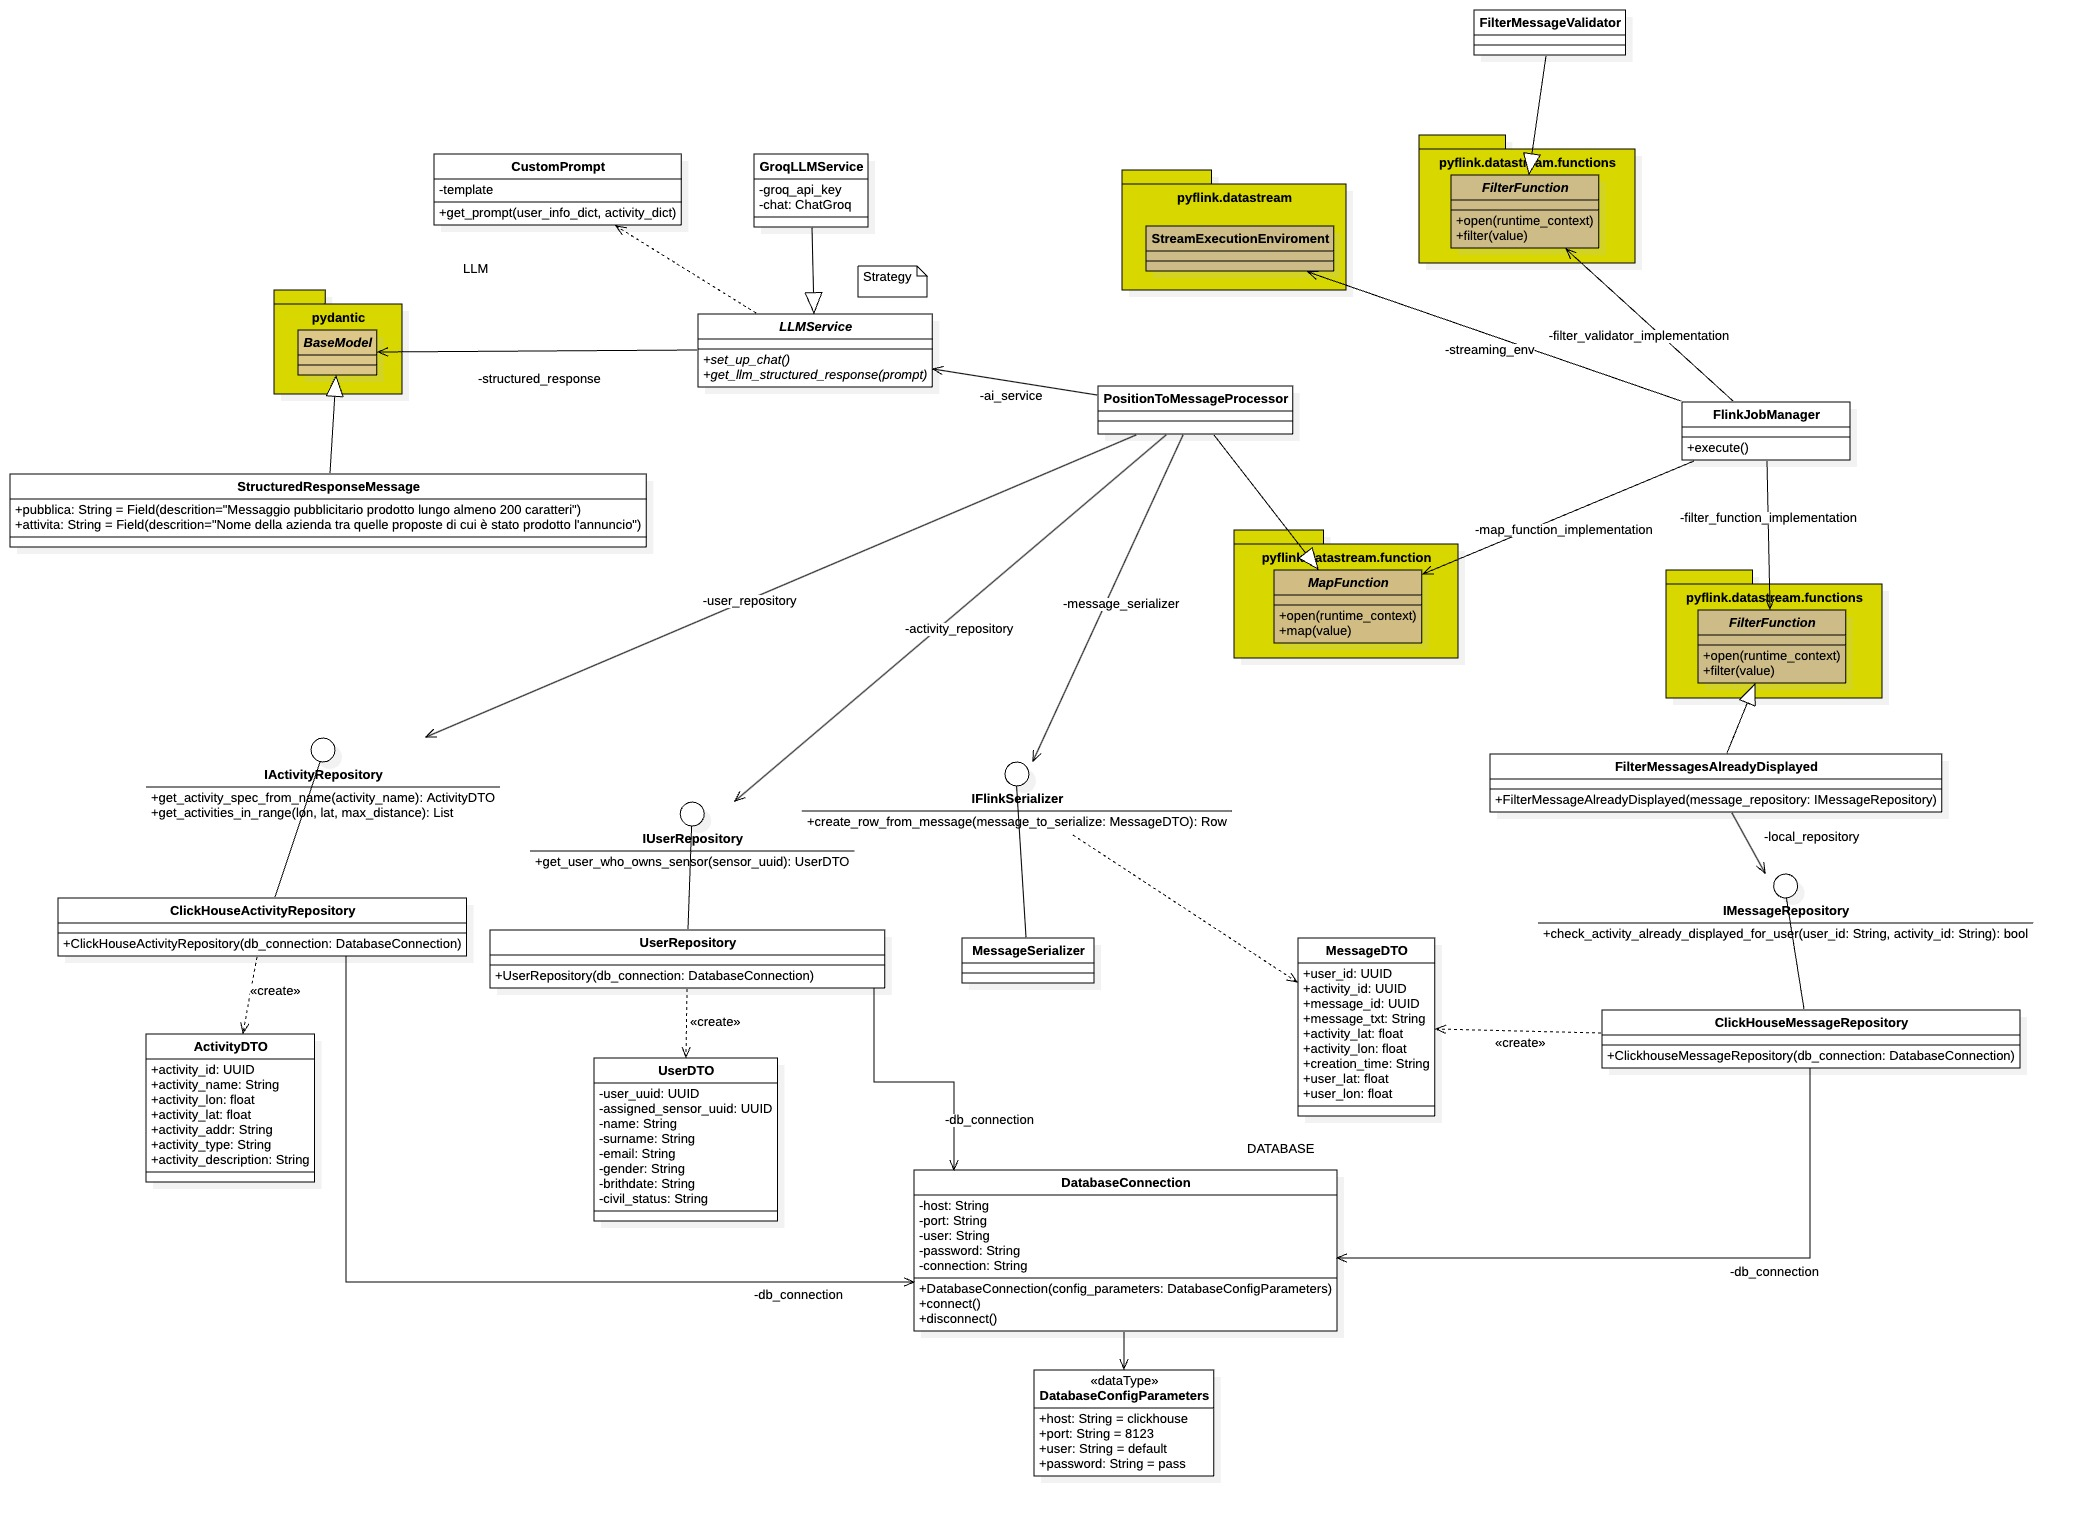
\includegraphics[width=1.24\textwidth]{flink2.jpg}
        \caption{PositionToMessageProcessorService InBound/OutBound Ports con il Broker}
        \end{figure}

        \begin{figure}[H]
        \hspace{-1.5cm}
        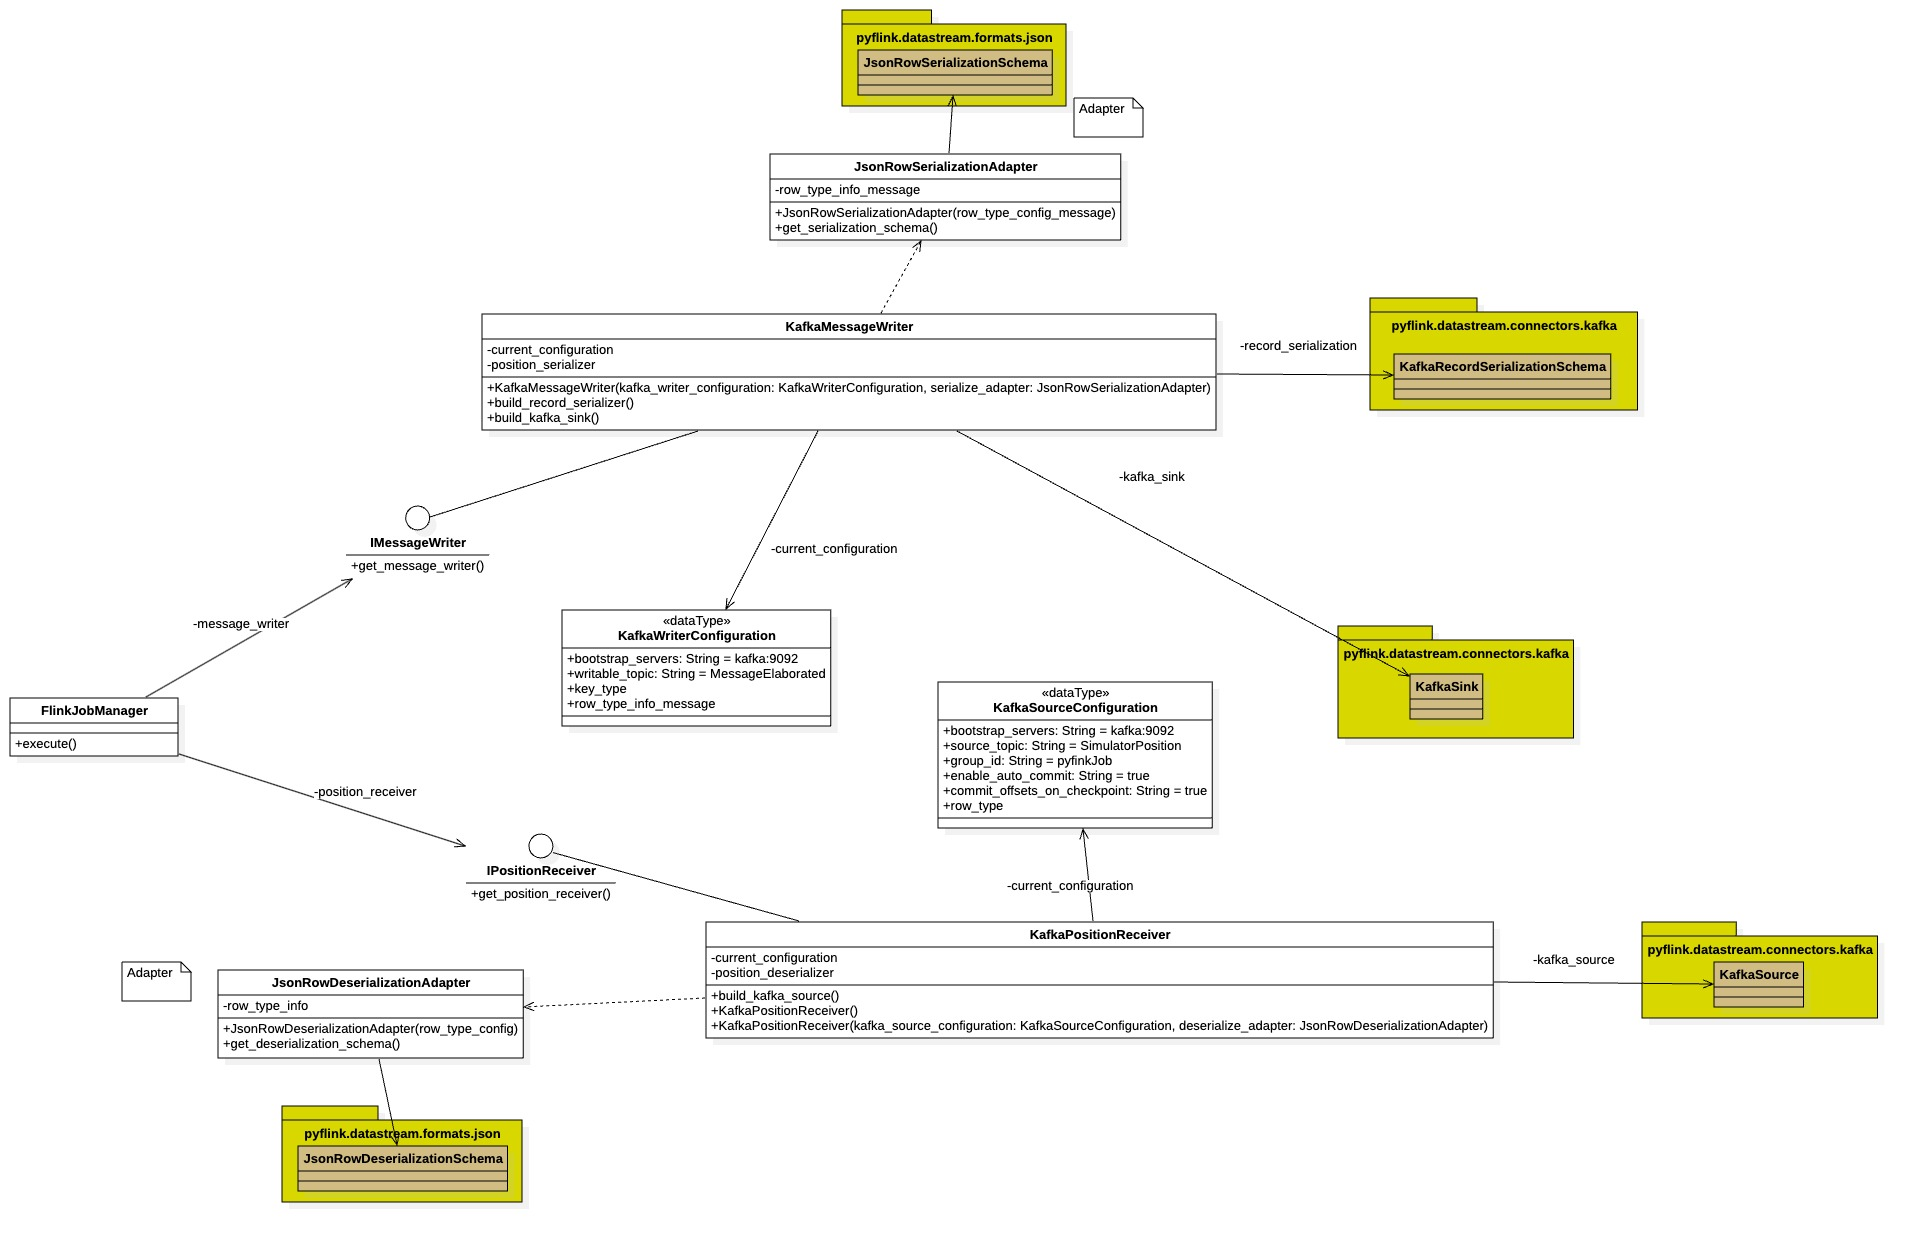
\includegraphics[width=1.25\textwidth]{flink1.jpg}
        \caption{PositionToMessageProcessorService OutBound Ports}
        \end{figure}

        
    \paragraph{Design Pattern - Adapter Pattern}
    \begin{itemize} 
    \item \textbf{Motivazioni e studio del design pattern}
    \begin{itemize}
        \item Nel contesto della nostra architettura esagonale, l'Adapter Pattern risulta essenziale per facilitare l'interazione tra la business logic e le componenti esterne (ad esempio, i servizi di pubblicazione su Kafka o la ricezione di dati da esso).
        \item Grazie a questo approccio, manteniamo l'indipendenza tra i moduli interni e le librerie di terze parti, riducendo i vincoli e semplificando la futura sostituzione di tali componenti senza impattare sul sistema.
        \item Questo pattern consente di adattare interfacce incompatibili e promuove il riutilizzo del codice, proteggendo la logica di business dai dettagli implementativi delle tecnologie esterne.
    \end{itemize}
    
    \item \textbf{Implementazione del design pattern}
    \begin{itemize}
        \item L'implementazione del pattern Adapter avviene tramite:
        \begin{enumerate}
            \item Interfacce ben definite (\texttt{IMessageWriter} e \texttt{IPositionReceiver}) che dichiarano i metodi essenziali per l'interazione con l'architettura esagonale
            \item Classi adapter concrete (\texttt{KafkaMessageWriter} e \texttt{KafkaPositionReceiver}) che implementano tali interfacce, incapsulando la complessità di conversione tra i formati interni e quelli richiesti da Kafka
            \item Adapter di serializzazione/deserializzazione (\texttt{JsonRowSerializationAdapter} e \\ \texttt{JsonRowDeserializationAdapter}) che gestiscono la conversione dei dati
        \end{enumerate}
    \end{itemize}
    
    \item \textbf{Integrazione del pattern}
    \begin{itemize}
        \item \texttt{KafkaMessageWriter} agisce come adapter per l'invio di messaggi a Kafka:
        \begin{enumerate}
            \item Riceve una configurazione (\texttt{KafkaWriterConfiguration}) e un adapter di serializzazione
            \item Costruisce un serializzatore di record Kafka configurandolo con il topic di destinazione e gli schemi di serializzazione per chiave e valore
            \item Crea un sink Kafka con i server bootstrap e il serializzatore configurati
            \item Espone il metodo \texttt{get\_message\_writer()} che restituisce il sink configurato, nascondendo tutti i dettagli di implementazione di Kafka
        \end{enumerate}
        
        \item \texttt{KafkaPositionReceiver} agisce come adapter per la ricezione di posizioni da Kafka:
        \begin{enumerate}
            \item Riceve una configurazione (\texttt{KafkaSourceConfiguration}) e un adapter di deserializzazione
            \item Costruisce una sorgente Kafka configurandola con server bootstrap, topic, gruppo consumer e schema di deserializzazione
            \item Configura proprietà specifiche come auto-commit e gestione degli offset
            \item Espone il metodo \texttt{get\_position\_receiver()} che restituisce la sorgente configurata, nascondendo i dettagli di Kafka
        \end{enumerate}
        
        \item Grazie a questi adapter, il core dell'applicazione può interagire con Kafka attraverso un'interfaccia semplificata e coerente, senza essere esposto ai dettagli implementativi della libreria Kafka. Se in futuro fosse necessario sostituire Kafka con un altro broker di messaggistica, basterebbe implementare nuovi adapter che rispettino le stesse interfacce.
    \end{itemize}
    \end{itemize}

    \paragraph{Design Pattern - Strategy Pattern}
    \begin{itemize} 
    \item \textbf{Motivazioni e studio del design pattern}
    \begin{itemize}
        \item Nel contesto della nostra architettura, il Pattern Strategy risulta fondamentale per gestire diverse implementazioni di modelli linguistici (LLM) senza modificare il codice client che li utilizza.
        \item Questo pattern permette di definire una famiglia di algoritmi (in questo caso, diverse implementazioni di servizi LLM), incapsularli in classi separate e renderli intercambiabili a runtime.
        \item Grazie a questo approccio, possiamo estendere facilmente le capacità del sistema aggiungendo nuovi servizi LLM senza modificare la logica di business che li utilizza, garantendo una maggiore flessibilità e manutenibilità del codice.
    \end{itemize}
    
    \item \textbf{Implementazione del design pattern}
    \begin{itemize}
        \item L'implementazione del pattern Strategy avviene tramite:
        \begin{enumerate}
            \item Un'interfaccia astratta \texttt{LLMService} che definisce il contratto comune per tutti i servizi LLM, dichiarando i metodi essenziali come \texttt{set\_up\_chat()} e \texttt{get\_llm\_structured\_response()}.
            \item Classi concrete (come \texttt{GroqLLMService}) che implementano l'interfaccia \texttt{LLMService}, fornendo implementazioni specifiche per interagire con diversi provider di LLM.
            \item Un meccanismo di configurazione che permette di selezionare la strategia appropriata a runtime.
        \end{enumerate}
    \end{itemize}
    
    \item \textbf{Integrazione del pattern}
    \begin{itemize}
        \item \texttt{LLMService} agisce come interfaccia strategica:
        \begin{enumerate}
            \item Definisce un costruttore che riceve un modello strutturato di risposta (\texttt{structured\_response})
            \item Dichiara il metodo astratto \texttt{set\_up\_chat()} che deve essere implementato per inizializzare la comunicazione con il servizio LLM specifico
            \item Dichiara il metodo astratto \texttt{get\_llm\_structured\_response(prompt)} che deve essere implementato per ottenere risposte strutturate dal LLM
        \end{enumerate}
        
        \item \texttt{GroqLLMService} rappresenta una strategia concreta:
        \begin{enumerate}
            \item Implementa l'interfaccia \texttt{LLMService} fornendo un'implementazione specifica per il servizio Groq
            \item Configura parametri specifici come la chiave API, il modello ("Gemma2-9b-it"), la temperatura e altri parametri propri di Groq
            \item Implementa \texttt{set\_up\_chat()} impostando un limitatore di frequenza e inizializzando il client ChatGroq
            \item Implementa \texttt{get\_llm\_structured\_response(prompt)} utilizzando la funzionalità \texttt{with\_structured\_output} di ChatGroq per ottenere risposte nel formato desiderato
        \end{enumerate}
        
        \item Il client (in questo caso, \texttt{PositionToMessageProcessor}) interagisce con l'interfaccia \texttt{LLMService} senza conoscere quale implementazione specifica viene utilizzata:
        \begin{enumerate}
            \item Riceve un'istanza di \texttt{LLMService} tramite dependency injection
            \item Chiama il metodo \texttt{get\_llm\_structured\_response()} sull'interfaccia, delegando l'implementazione concreta alla strategia selezionata
            \item Non ha bisogno di conoscere i dettagli implementativi di Groq o di qualsiasi altro servizio LLM
        \end{enumerate}
        
        \item Grazie a questo pattern, il sistema può facilmente supportare nuovi servizi LLM (come OpenAI, Claude, ecc.) semplicemente creando nuove classi che implementano l'interfaccia \texttt{LLMService}, senza modificare il codice che utilizza questi servizi. Ciò garantisce un'elevata estensibilità e facilità di manutenzione.
    \end{itemize}
    \end{itemize}


    \myparagraph{Classi, interfacce, metodi e attributi:}

    \paragraph{FlinkJobManager}
    \begin{itemize} 
    \item \textbf{Descrizione}: Implementa un gestore per job Apache Flink che configura e orchestra un pipeline di elaborazione dati in streaming. Costruisce un flusso di dati completo con operazioni di ricezione, trasformazione e invio di messaggi.
    \item \textbf{Attributi}:
    \begin{itemize}
        \item \texttt{\_\_streaming\_env: StreamExecutionEnvironment} - Ambiente di esecuzione Flink per l'elaborazione in streaming.
        \item \texttt{\_\_populated\_datastream} - Stream di dati iniziale popolato dalla sorgente di posizioni.
        \item \texttt{\_\_keyed\_stream} - Stream partizionato (keyed) in base all'identificatore della posizione.
        \item \texttt{\_\_validated\_stream} - Stream filtrato contenente solo le posizioni validate.
        \item \texttt{\_\_mapped\_stream} - Stream con dati trasformati dal formato di input al formato di output.
        \item \texttt{\_\_filtered\_stream} - Stream finale filtrato prima dell'invio al sink.
    \end{itemize}
    
    \item \textbf{Operazioni}:
    \begin{itemize}
        \item \texttt{\_\_init\_\_(self, streaming\_env\_istance: StreamExecutionEnvironment, map\_function\_implementation: MapFunction, filter\_validator\_implementation: FilterFunction, filter\_function\_implementation: FilterFunction, position\_receiver\_istance: IPositionReceiver, message\_sender\_istance: IMessageWriter)} - Costruttore che configura l'intero pipeline di elaborazione dati. Inizializza l'ambiente di streaming, crea uno stream di dati dalla sorgente, applica operazioni di chiave, validazione, mappatura e filtraggio, e configura il sink per l'output.
        
        \item \texttt{execute(self)} - Avvia l'esecuzione del job Flink con l'identificatore "Flink Job".
    \end{itemize}
    \end{itemize}

    \paragraph{IMessageWriter}
    \begin{itemize} 
    \item \textbf{Descrizione}: Implementa un'interfaccia astratta che definisce il contratto per i componenti di scrittura dei messaggi. Rappresenta una porta in uscita (outbound port) nel sistema, responsabile di fornire un meccanismo standardizzato per scrivere messaggi verso sistemi esterni.
    \item \textbf{Attributi}:
    \begin{itemize}
        \item Nessun attributo definito a livello di interfaccia.
    \end{itemize}
    
    \item \textbf{Operazioni}:
    \begin{itemize}
        \item \texttt{get\_message\_writer(self)} - Metodo astratto che deve essere implementato dalle sottoclassi per fornire l'istanza concreta dello scrittore di messaggi. L'implementazione dipenderà dal sistema di destinazione specifico (ad esempio, un sink Kafka o un altro sistema di messaggistica).
    \end{itemize}
    \end{itemize}

    \paragraph{KafkaMessageWriter}
    \begin{itemize} 
    \item \textbf{Descrizione}: Implementa l'interfaccia IMessageWriter per fornire un adattatore specifico per la scrittura di messaggi su Apache Kafka. Configura e costruisce un sink Kafka per l'integrazione con il pipeline di elaborazione dati di Apache Flink.
    \item \textbf{Attributi}:
    \begin{itemize}
        \item \texttt{\_\_current\_configuration: KafkaWriterConfiguration} - Configurazione contenente i parametri necessari per la connessione a Kafka e la serializzazione dei messaggi.
        \item \texttt{\_\_position\_serializer} - Schema di serializzazione per convertire gli oggetti di posizione in formato JSON.
        \item \texttt{\_\_record\_serializer: KafkaRecordSerializationSchema} - Schema di serializzazione per i record Kafka che include sia la chiave che il valore.
        \item \texttt{\_\_kafka\_sink: KafkaSink} - Componente sink di Flink configurato per scrivere su Kafka.
    \end{itemize}
    
    \item \textbf{Operazioni}:
    \begin{itemize}
        \item \texttt{\_\_init\_\_(self, kafka\_writer\_configuration: KafkaWriterConfiguration, serialize\_adapter: JsonRowSerializationAdapter)} - Costruttore che inizializza l'adattatore con la configurazione Kafka e l'adattatore di serializzazione JSON, e costruisce il serializzatore di record e il sink Kafka.
        
        \item \texttt{build\_record\_serializer(self)} - Metodo privato che costruisce lo schema di serializzazione per i record Kafka, configurando il topic di destinazione, lo schema di serializzazione della chiave e dello schema di serializzazione del valore.
        
        \item \texttt{build\_kafka\_sink(self)} - Metodo privato che costruisce il sink Kafka utilizzando i server bootstrap e il serializzatore di record precedentemente configurati.
        
        \item \texttt{get\_message\_writer(self)} - Implementazione del metodo dell'interfaccia che restituisce l'istanza del sink Kafka configurato, pronto per essere utilizzato nel pipeline Flink.
    \end{itemize}
    \end{itemize}

    \paragraph{JsonRowSerializationAdapter}
    \begin{itemize} 
    \item \textbf{Descrizione}: Implementa un adattatore per la serializzazione di dati in formato JSON. Incapsula la configurazione e la creazione di uno schema di serializzazione JSON per l'uso nei flussi di dati di Apache Flink.
    \item \textbf{Attributi}:
    \begin{itemize}
        \item \texttt{\_\_row\_type\_info\_message} - Informazioni sul tipo di riga che definisce la struttura dei dati da serializzare. Specifica lo schema e i tipi di dati per il processo di serializzazione JSON.
    \end{itemize}
    
    \item \textbf{Operazioni}:
    \begin{itemize}
        \item \texttt{\_\_init\_\_(self, row\_type\_config\_message)} - Costruttore che inizializza l'adattatore con le informazioni di tipo necessarie per definire la struttura dei messaggi da serializzare.
        
        \item \texttt{get\_serialization\_schema(self)} - Restituisce uno schema di serializzazione JSON configurato con le informazioni di tipo fornite. Lo schema creato può essere utilizzato per convertire oggetti Flink Row in stringhe JSON formattate secondo lo schema definito.
    \end{itemize}
    \end{itemize}

    \paragraph{KafkaWriterConfiguration}
    \begin{itemize} 
    \item \textbf{Descrizione}: Implementa una classe di dati (dataclass) che contiene la configurazione necessaria per scrivere messaggi su Apache Kafka dal pipeline Flink. Definisce sia i parametri di connessione sia la struttura dei dati da serializzare.
    \item \textbf{Attributi}:
    \begin{itemize}
        \item \texttt{bootstrap\_servers: str} - Indirizzo e porta dei server bootstrap Kafka. Il valore predefinito è "kafka:9092".
        \item \texttt{writable\_topic: str} - Nome del topic Kafka su cui scrivere i messaggi elaborati. Il valore predefinito è "MessageElaborated".
        \item \texttt{key\_type} - Definizione del tipo di chiave per i record Kafka, strutturata come una riga con un singolo campo 'user\_uuid' di tipo stringa.
        \item \texttt{row\_type\_info\_message} - Definizione completa dello schema dei messaggi, strutturata come una riga con nove campi che rappresentano le informazioni dell'utente, dell'attività e del messaggio, con i relativi tipi di dati (stringhe per identificatori e messaggio, float per coordinate geografiche).
    \end{itemize}
    
    \item \textbf{Operazioni}:
    \begin{itemize}
        \item Nessuna operazione esplicita definita, in quanto si tratta di una dataclass che fornisce automaticamente costruttore, rappresentazione in stringa, confronto e altre funzionalità.
    \end{itemize}
    \end{itemize}


    \paragraph{IPositionReceiver}
    \begin{itemize} 
    \item \textbf{Descrizione}: Implementa un'interfaccia astratta che definisce il contratto per i componenti di ricezione delle posizioni. Rappresenta una porta in entrata (inbound port) nel sistema, responsabile di fornire un meccanismo standardizzato per ricevere dati di posizione da fonti esterne.
    \item \textbf{Attributi}:
    \begin{itemize}
        \item Nessun attributo definito a livello di interfaccia.
    \end{itemize}
    
    \item \textbf{Operazioni}:
    \begin{itemize}
        \item \texttt{get\_position\_receiver(self)} - Metodo astratto che deve essere implementato dalle sottoclassi per fornire l'istanza concreta del ricevitore di posizioni. L'implementazione dipenderà dalla fonte di dati specifica (ad esempio, un source Kafka o un altro sistema di messaggistica).
    \end{itemize}
    \end{itemize}


    \paragraph{KafkaPositionReceiver}
    \begin{itemize} 
    \item \textbf{Descrizione}: Implementa l'interfaccia IPositionReceiver per fornire un adattatore specifico per la ricezione di posizioni da Apache Kafka. Configura e costruisce una fonte Kafka per l'integrazione con il pipeline di elaborazione dati di Apache Flink.
    \item \textbf{Attributi}:
    \begin{itemize}
        \item \texttt{\_\_current\_configuration: KafkaSourceConfiguration} - Configurazione contenente i parametri necessari per la connessione a Kafka e la deserializzazione dei messaggi.
        \item \texttt{\_\_position\_deserializer} - Schema di deserializzazione per convertire i messaggi JSON ricevuti in oggetti di posizione.
        \item \texttt{\_\_kafka\_source: KafkaSource} - Componente source di Flink configurato per leggere da Kafka.
    \end{itemize}
    
    \item \textbf{Operazioni}:
    \begin{itemize}
        \item \texttt{\_\_init\_\_(self, kafka\_source\_configuration: KafkaSourceConfiguration, deserialize\_adapter: JsonRowDeserializationAdapter)} - Costruttore che inizializza l'adattatore con la configurazione Kafka e l'adattatore di deserializzazione JSON, e costruisce la fonte Kafka.
        
        \item \texttt{build\_kafka\_source(self) -> KafkaSource} - Metodo privato che costruisce la fonte Kafka configurando i server bootstrap, il topic di origine, l'ID del gruppo di consumatori, il deserializzatore e altre proprietà specifiche come l'auto-commit e il commit degli offset sui checkpoint.
        
        \item \texttt{get\_position\_receiver(self)} - Implementazione del metodo dell'interfaccia che restituisce l'istanza della fonte Kafka configurata, pronta per essere utilizzata nel pipeline Flink.
    \end{itemize}
    \end{itemize}

    \paragraph{JsonRowDeserializationAdapter}
    \begin{itemize} 
    \item \textbf{Descrizione}: Implementa un adattatore per la deserializzazione di dati in formato JSON. Incapsula la configurazione e la creazione di uno schema di deserializzazione JSON per l'uso nei flussi di dati di Apache Flink.
    \item \textbf{Attributi}:
    \begin{itemize}
        \item \texttt{\_\_row\_type\_info} - Informazioni sul tipo di riga che definisce la struttura dei dati da deserializzare. Specifica lo schema e i tipi di dati per il processo di deserializzazione JSON.
    \end{itemize}
    
    \item \textbf{Operazioni}:
    \begin{itemize}
        \item \texttt{\_\_init\_\_(self, row\_type\_config)} - Costruttore che inizializza l'adattatore con le informazioni di tipo necessarie per definire la struttura dei messaggi da deserializzare.
        
        \item \texttt{get\_deserialization\_schema(self)} - Restituisce uno schema di deserializzazione JSON configurato con le informazioni di tipo fornite. Lo schema creato può essere utilizzato per convertire stringhe JSON in oggetti Flink Row strutturati secondo lo schema definito.
    \end{itemize}
    \end{itemize}

    \paragraph{KafkaSourceConfiguration}
    \begin{itemize} 
    \item \textbf{Descrizione}: Implementa una classe di dati (dataclass) che contiene la configurazione necessaria per leggere messaggi da Apache Kafka nel pipeline Flink. Definisce sia i parametri di connessione sia la struttura dei dati da deserializzare.
    \item \textbf{Attributi}:
    \begin{itemize}
        \item \texttt{bootstrap\_servers: str} - Indirizzo e porta dei server bootstrap Kafka. Il valore predefinito è "kafka:9092".
        \item \texttt{source\_topic: str} - Nome del topic Kafka da cui leggere i messaggi di posizione. Il valore predefinito è "SimulatorPosition".
        \item \texttt{group\_id: str} - Identificatore del gruppo di consumatori Kafka. Il valore predefinito è "pyfinkJob".
        \item \texttt{enable\_auto\_commit: str} - Flag che indica se abilitare il commit automatico degli offset. Il valore predefinito è "true".
        \item \texttt{commit\_offsets\_on\_checkpoint: str} - Flag che indica se commettere gli offset durante i checkpoint Flink. Il valore predefinito è "true".
        \item \texttt{row\_type} - Definizione dello schema di deserializzazione delle posizioni, strutturato come una riga con quattro campi: 'user\_uuid' (string), 'latitude' (float), 'longitude' (float) e 'received\_at' (string).
    \end{itemize}
    
    \item \textbf{Operazioni}:
    \begin{itemize}
        \item Nessuna operazione esplicita definita, in quanto si tratta di una dataclass che fornisce automaticamente costruttore, rappresentazione in stringa, confronto e altre funzionalità.
    \end{itemize}
    \end{itemize}
    
    \paragraph{FilterMessageValidator}
    \begin{itemize} 
    \item \textbf{Descrizione}: Implementa la classe FilterFunction di Apache Flink per filtrare messaggi Kafka invalidi o potenzialmente dannosi. Esegue diversi controlli di validazione sui dati ricevuti per garantire l'integrità e la sicurezza del pipeline di elaborazione.
    \item \textbf{Attributi}:
    \begin{itemize}
        \item Nessun attributo specifico definito nella classe.
    \end{itemize}
    
    \item \textbf{Operazioni}:
    \begin{itemize}
        \item \texttt{open(self, runtime\_context)} - Metodo che viene chiamato all'inizializzazione della funzione di filtro. Non implementa operazioni specifiche in questa versione.
        
        \item \texttt{filter(self, value)} - Implementa il metodo dell'interfaccia FilterFunction per determinare quali messaggi devono essere mantenuti nel flusso. Esegue diversi controlli di validazione:
        \begin{itemize}
            \item Verifica che latitudine e longitudine siano valori numerici e rientrino nei range geografici validi (-90 <= lat <= 90, -180 <= lon <= 180).
            \item Controlla che il timestamp sia in un formato valido ('%Y-%m-%d %H:%M:%S').
            \item Verifica che l'ID utente sia un UUID valido di versione 4.
            \item Analizza tutti i valori di tipo stringa per identificare pattern sospetti di SQL injection (come "--", ";", comandi SQL come "DROP", "DELETE", ecc.).
        \end{itemize}
        Restituisce True solo se tutti i controlli di validazione vengono superati, altrimenti restituisce False per scartare il messaggio dal flusso.
    \end{itemize}
    \end{itemize}

    \paragraph{PositionToMessageProcessor}
    \begin{itemize} 
    \item \textbf{Descrizione}: Implementa la classe MapFunction di Apache Flink per trasformare dati di posizione in messaggi personalizzati. Utilizza un servizio di intelligenza artificiale per generare contenuti pubblicitari contestuali basati sulla posizione dell'utente e sulle attività disponibili nelle vicinanze.
    \item \textbf{Attributi}:
    \begin{itemize}
        \item \texttt{ai\_service: LLMService} - Servizio di modello di linguaggio (LLM) utilizzato per generare contenuti pubblicitari personalizzati.
        \item \texttt{\_\_user\_repository: IUserRepository} - Repository per accedere alle informazioni sugli utenti.
        \item \texttt{\_\_activity\_repository: IActivityRepository} - Repository per recuperare attività commerciali nelle vicinanze dell'utente.
        \item \texttt{\_\_message\_serializer: IFlinkSerializable} - Componente per serializzare i messaggi nel formato richiesto da Flink.
        \item \texttt{prompt\_creator: CustomPrompt} - Generatore di prompt per l'interazione con il servizio LLM.
    \end{itemize}
    
    \item \textbf{Operazioni}:
    \begin{itemize}
        \item \texttt{\_\_init\_\_(self, ai\_chatbot\_service: LLMService, user\_repository: IUserRepository, activity\_repository: IActivityRepository, message\_serializer: IFlinkSerializable)} - Costruttore che inizializza il processore con i servizi e repository necessari.
        
        \item \texttt{open(self, runtime\_context)} - Metodo chiamato all'inizializzazione del pipeline Flink. Configura il servizio LLM e inizializza il generatore di prompt.
        
        \item \texttt{map(self, value)} - Implementa il metodo dell'interfaccia MapFunction per trasformare i dati di posizione in messaggi. Esegue il seguente processo:
        \begin{itemize}
            \item Recupera le informazioni dell'utente associato al sensore
            \item Trova le attività commerciali nel raggio di 300 metri dalla posizione
            \item Se non ci sono attività nelle vicinanze, restituisce un messaggio segnaposto
            \item Altrimenti, genera un prompt personalizzato basato sull'utente e sulle attività
            \item Invoca il servizio LLM per ottenere una risposta strutturata
            \item Recupera le informazioni dettagliate sull'attività selezionata
            \item Crea un oggetto MessageDTO con il contenuto pubblicitario generato
            \item Serializza il messaggio nel formato Row di Flink per l'elaborazione successiva
        \end{itemize}
    \end{itemize}
    \end{itemize}



    \paragraph{LLMService}
    \begin{itemize} 
    \item \textbf{Descrizione}: Implementa un'interfaccia astratta che definisce il contratto per servizi di modelli linguistici (LLM). Fornisce una struttura comune per interagire con diversi modelli di linguaggio e ottenere risposte strutturate in un formato predefinito.
    \item \textbf{Attributi}:
    \begin{itemize}
        \item \texttt{\_llm\_structured\_response: BaseModel} - Modello Pydantic che definisce la struttura attesa per la risposta del modello linguistico.
    \end{itemize}
    
    \item \textbf{Operazioni}:
    \begin{itemize}
        \item \texttt{\_\_init\_\_(self, structured\_response: BaseModel)} - Costruttore che inizializza il servizio con un modello Pydantic che definisce la struttura della risposta attesa dal modello linguistico.
        
        \item \texttt{set\_up\_chat(self)} - Metodo astratto che deve essere implementato dalle sottoclassi per inizializzare e configurare la sessione di chat con il modello linguistico.
        
        \item \texttt{get\_llm\_structured\_response(self, prompt)} - Metodo astratto che deve essere implementato dalle sottoclassi per inviare un prompt al modello linguistico e ottenere una risposta strutturata secondo il modello Pydantic definito.
    \end{itemize}
    \end{itemize}

    \paragraph{CustomPrompt}
    \begin{itemize} 
    \item \textbf{Descrizione}: Implementa un generatore di prompt personalizzati per l'interazione con modelli linguistici. Utilizza un template predefinito per costruire richieste strutturate che mirano a ottenere messaggi pubblicitari contestualizzati in base alle informazioni dell'utente e alle attività commerciali disponibili.
    \item \textbf{Attributi}:
    \begin{itemize}
        \item \texttt{\_\_template: Template} - Template di stringa che definisce la struttura del prompt, con variabili per inserire dinamicamente informazioni sull'utente e sulle attività commerciali.
    \end{itemize}
    
    \item \textbf{Operazioni}:
    \begin{itemize}
        \item \texttt{\_\_init\_\_(self)} - Costruttore che inizializza il generatore di prompt con un template predefinito. Il template include istruzioni per il modello linguistico su come generare un messaggio pubblicitario personalizzato, con criteri specifici per la selezione dell'attività e vincoli sul formato della risposta.
        
        \item \texttt{get\_prompt(self, user\_info\_dict, activity\_dict)} - Genera un prompt personalizzato sostituendo le variabili del template con le informazioni specifiche dell'utente e l'elenco delle attività disponibili. Formatta le attività come una lista puntata e restituisce il prompt completo pronto per essere inviato al modello linguistico.
    \end{itemize}
    \end{itemize}

    \paragraph{StructuredResponseMessage}
    \begin{itemize} 
    \item \textbf{Descrizione}: Implementa un modello Pydantic che definisce la struttura della risposta attesa dal modello linguistico. Garantisce che le risposte generate soddisfino un formato predefinito, facilitando l'elaborazione e la validazione automatica dei dati ricevuti.
    \item \textbf{Attributi}:
    \begin{itemize}
        \item \texttt{pubblicita: str} - Campo che contiene il messaggio pubblicitario generato dal modello linguistico. Deve essere lungo almeno 200 caratteri come specificato nella descrizione del campo.
        \item \texttt{attivita: str} - Campo che contiene il nome dell'azienda selezionata tra quelle proposte per cui è stato prodotto l'annuncio pubblicitario.
    \end{itemize}
    
    \item \textbf{Operazioni}:
    \begin{itemize}
        \item Nessuna operazione esplicita definita, in quanto si tratta di un modello Pydantic che fornisce automaticamente funzionalità di validazione, serializzazione, deserializzazione e altre funzionalità di gestione dei dati.
    \end{itemize}
    \end{itemize}


    \paragraph{GroqLLMService}
    \begin{itemize} 
    \item \textbf{Descrizione}: Implementa una classe concreta che estende l'interfaccia LLMService per interagire specificamente con l'API Groq. Configura e gestisce una connessione a un modello linguistico di Groq, con controllo della frequenza delle richieste e gestione delle risposte strutturate.
    \item \textbf{Attributi}:
    \begin{itemize}
        \item \texttt{\_\_groq\_api\_key: str} - Chiave API per autenticarsi al servizio Groq, recuperata dalle variabili d'ambiente.
        \item \texttt{\_\_chat: ChatGroq} - Istanza del client di chat Groq configurata con parametri specifici per l'interazione con il modello linguistico.
    \end{itemize}
    
    \item \textbf{Operazioni}:
    \begin{itemize}
        \item \texttt{\_\_init\_\_(self, structured\_response)} - Costruttore che inizializza il servizio ereditando dalla classe base e configurando la chiave API Groq dalle variabili d'ambiente.
        
        \item \texttt{set\_up\_chat(self)} - Implementa il metodo astratto della classe base per inizializzare il client di chat Groq. Configura un rate limiter per controllare la frequenza delle richieste API (circa una ogni 15 secondi) e inizializza il client ChatGroq con parametri specifici come il modello "Gemma2-9b-it", temperatura di generazione, e altre configurazioni per la gestione delle richieste.
        
        \item \texttt{get\_llm\_structured\_response(self, prompt)} - Implementa il metodo astratto della classe base per inviare un prompt al modello Groq e ottenere una risposta strutturata. Utilizza la funzionalità "with\_structured\_output" del client ChatGroq per forzare la risposta nel formato definito dal modello Pydantic specificato nella classe base.
    \end{itemize}
    \end{itemize}


    \paragraph{IActivityRepository}
    \begin{itemize} 
    \item \textbf{Descrizione}: Implementa un'interfaccia astratta che definisce il contratto per i repository di gestione delle attività commerciali. Stabilisce i metodi necessari per recuperare informazioni sulle attività in base al nome o alla posizione geografica.
    \item \textbf{Attributi}:
    \begin{itemize}
        \item Nessun attributo definito a livello di interfaccia.
    \end{itemize}
    
    \item \textbf{Operazioni}:
    \begin{itemize}
        \item \texttt{get\_activity\_spec\_from\_name(self, activity\_name) -> ActivityDTO} - Metodo astratto che deve essere implementato dalle sottoclassi per recuperare le specifiche dettagliate di un'attività commerciale in base al suo nome. Restituisce un oggetto ActivityDTO contenente tutte le informazioni sull'attività.
        
        \item \texttt{get\_activities\_in\_range(self, lon, lat, max\_distance) -> list} - Metodo astratto che deve essere implementato dalle sottoclassi per recuperare un elenco di attività commerciali situate entro una distanza massima specificata da una data posizione geografica. Prende in input le coordinate (longitudine e latitudine) e la distanza massima, e restituisce una lista di attività nelle vicinanze.
    \end{itemize}
    \end{itemize}

    \paragraph{ClickhouseActivityRepository}
    \begin{itemize} 
    \item \textbf{Descrizione}: Implementa la classe concreta che realizza l'interfaccia IActivityRepository per recuperare informazioni sulle attività commerciali da un database ClickHouse. Fornisce metodi per cercare attività in base alla vicinanza geografica e al nome.
    \item \textbf{Attributi}:
    \begin{itemize}
        \item \texttt{\_\_db\_conn: DatabaseConnection} - Connessione al database ClickHouse utilizzata per eseguire query sui dati delle attività.
    \end{itemize}
    
    \item \textbf{Operazioni}:
    \begin{itemize}
        \item \texttt{\_\_init\_\_(self, db\_connection: DatabaseConnection)} - Costruttore che inizializza il repository con una connessione al database.
        
        \item \texttt{get\_activities\_in\_range(self, lon, lat, max\_distance) -> list} - Implementa il metodo dell'interfaccia per trovare attività commerciali entro una distanza specificata da una posizione geografica. Esegue una query SQL che utilizza la funzione geoDistance per calcolare la distanza tra la posizione fornita e ogni attività, restituendo quelle che si trovano entro la distanza massima specificata. Il risultato comprende nome, indirizzo, tipo, descrizione e distanza calcolata.
        
        \item \texttt{get\_activity\_spec\_from\_name(self, activity\_name) -> ActivityDTO} - Implementa il metodo dell'interfaccia per recuperare i dettagli completi di un'attività in base al suo nome. Esegue una query SQL che cerca un'attività con il nome esatto fornito e costruisce un oggetto ActivityDTO con tutti i dati recuperati (UUID, nome, coordinate, indirizzo, tipo e descrizione). Se nessuna attività corrisponde al nome, restituisce un ActivityDTO vuoto.
    \end{itemize}
    \end{itemize}
    

    \paragraph{ActivityDTO}
    \begin{itemize} 
    \item \textbf{Descrizione}: Implementa un oggetto di trasferimento dati (Data Transfer Object) per la classe Activity. Viene utilizzato per astrarre e incapsulare i dati delle attività commerciali, facilitando il trasferimento delle informazioni tra i diversi strati dell'applicazione senza esporre i dettagli implementativi.
    \item \textbf{Attributi}:
    \begin{itemize}
        \item \texttt{activity\_id: uuid} - Identificatore univoco dell'attività commerciale.
        \item \texttt{activity\_name: str} - Nome dell'attività commerciale.
        \item \texttt{activity\_lon: float} - Longitudine della posizione geografica dell'attività.
        \item \texttt{activity\_lat: float} - Latitudine della posizione geografica dell'attività.
        \item \texttt{activity\_addr: str} - Indirizzo fisico dell'attività commerciale.
        \item \texttt{activity\_type: str} - Categoria o tipo di attività commerciale (es. Ristorante, Negozio, Servizio).
        \item \texttt{activity\_description: str} - Descrizione dettagliata dell'attività commerciale.
    \end{itemize}
    
    \item \textbf{Operazioni}:
    \begin{itemize}
        \item \texttt{\_\_init\_\_(self, activity\_id: uuid = uuid.uuid4(), activity\_name: str = "", activity\_lon: float = 0.0, activity\_lat: float = 0.0, activity\_addr: str ="", activity\_type: str = "", activity\_description: str ="")} - Costruttore che inizializza l'oggetto DTO con tutti i dati dell'attività, fornendo valori predefiniti per tutti i parametri in modo da poter istanziare anche un oggetto vuoto.
    \end{itemize}
    \end{itemize}
    
    \paragraph{IUserRepository}
    \begin{itemize} 
    \item \textbf{Descrizione}: Implementa un'interfaccia astratta che definisce il contratto per i repository di gestione degli utenti nel contesto dell'applicazione Flink. Stabilisce il metodo necessario per recuperare le informazioni di un utente in base all'identificatore del sensore associato.
    \item \textbf{Attributi}:
    \begin{itemize}
        \item Nessun attributo definito a livello di interfaccia.
    \end{itemize}
    
    \item \textbf{Operazioni}:
    \begin{itemize}
        \item \texttt{get\_user\_who\_owns\_sensor(self, sensor\_uuid) -> UserDTO} - Metodo astratto che deve essere implementato dalle sottoclassi per recuperare i dati dell'utente proprietario di un sensore specifico. Prende in input l'UUID del sensore e restituisce un oggetto UserDTO contenente tutte le informazioni dell'utente associato.
    \end{itemize}
    \end{itemize}

    \paragraph{ClickhouseUserRepository}
    \begin{itemize} 
    \item \textbf{Descrizione}: Implementa la classe concreta che realizza l'interfaccia IUserRepository per recuperare informazioni sugli utenti da un database ClickHouse. Fornisce un metodo per trovare un utente in base all'UUID del sensore a lui assegnato, recuperando anche i suoi interessi.
    \item \textbf{Attributi}:
    \begin{itemize}
        \item \texttt{\_\_db\_conn: DatabaseConnection} - Connessione al database ClickHouse utilizzata per eseguire query sui dati degli utenti.
    \end{itemize}
    
    \item \textbf{Operazioni}:
    \begin{itemize}
        \item \texttt{\_\_init\_\_(self, db\_connection: DatabaseConnection)} - Costruttore che inizializza il repository con una connessione al database.
        
        \item \texttt{get\_user\_who\_owns\_sensor(self, sensor\_uuid) -> UserDTO} - Implementa il metodo dell'interfaccia per recuperare i dati dell'utente associato a un sensore specifico. Esegue una query SQL complessa che unisce le tabelle user e user\_interest per ottenere tutti i dati dell'utente e i suoi interessi in un'unica operazione. La query filtra gli utenti in base all'UUID del sensore fornito, raggruppa i risultati per i campi dell'utente e utilizza la funzione groupArray per aggregare gli interessi in un array. Restituisce un oggetto UserDTO popolato con tutti i dati recuperati, incluso l'elenco degli interessi, o None se nessun utente è associato al sensore specificato.
    \end{itemize}
    \end{itemize}


    \paragraph{UserDTO}
    \begin{itemize} 
    \item \textbf{Descrizione}: Implementa un oggetto di trasferimento dati (Data Transfer Object) per la classe User nel contesto dell'applicazione Flink. Viene utilizzato per astrarre e incapsulare i dati degli utenti, facilitando il trasferimento delle informazioni tra i diversi strati dell'applicazione senza esporre i dettagli implementativi.
    \item \textbf{Attributi}:
    \begin{itemize}
        \item \texttt{user\_uuid: uuid} - Identificatore univoco dell'utente.
        \item \texttt{assigned\_sensor\_uuid: uuid} - Identificatore univoco del sensore assegnato all'utente.
        \item \texttt{name: str} - Nome dell'utente.
        \item \texttt{surname: str} - Cognome dell'utente.
        \item \texttt{email: str} - Indirizzo email dell'utente.
        \item \texttt{gender: str} - Genere dell'utente.
        \item \texttt{birthdate: str} - Data di nascita dell'utente.
        \item \texttt{civil\_status: str} - Stato civile dell'utente.
        \item \texttt{interests: list[str]} - Lista degli interessi dell'utente, opzionale (default None).
    \end{itemize}
    
    \item \textbf{Operazioni}:
    \begin{itemize}
        \item \texttt{\_\_init\_\_(self, user\_uuid: uuid, assigned\_sensor\_uuid: uuid, name: str, surname: str, email: str, gender: str, birthdate: str, civil\_status: str, interests: list[str] = None)} - Costruttore che inizializza l'oggetto DTO con tutti i dati dell'utente, includendo una lista opzionale di interessi che può essere None se non specificata.
    \end{itemize}
    \end{itemize}

    \paragraph{IMessageRepository}
    \begin{itemize} 
    \item \textbf{Descrizione}: Implementa un'interfaccia astratta che definisce il contratto per i repository di gestione dei messaggi. Stabilisce il metodo necessario per verificare se un'attività è già stata mostrata a un utente specifico, permettendo così di evitare ripetizioni nei messaggi pubblicitari.
    \item \textbf{Attributi}:
    \begin{itemize}
        \item Nessun attributo definito a livello di interfaccia.
    \end{itemize}
    
    \item \textbf{Operazioni}:
    \begin{itemize}
        \item \texttt{check\_activity\_already\_displayed\_for\_user(self, user\_id: str, activity\_id: str) -> bool} - Metodo astratto che deve essere implementato dalle sottoclassi per verificare se una specifica attività commerciale è già stata mostrata a un determinato utente. Prende in input l'identificatore dell'utente e l'identificatore dell'attività, e restituisce un valore booleano: True se l'attività è già stata mostrata all'utente, False altrimenti.
    \end{itemize}
    \end{itemize}


    \paragraph{ClickhouseMessageRepository}
    \begin{itemize} 
    \item \textbf{Descrizione}: Implementa la classe concreta che realizza l'interfaccia IMessageRepository per gestire i messaggi in un database ClickHouse. Fornisce funzionalità per verificare se un messaggio pubblicitario relativo a una specifica attività è già stato mostrato a un determinato utente.
    \item \textbf{Attributi}:
    \begin{itemize}
        \item \texttt{\_\_db\_conn: DatabaseConnection} - Connessione al database ClickHouse utilizzata per eseguire query sui dati dei messaggi.
    \end{itemize}
    
    \item \textbf{Operazioni}:
    \begin{itemize}
        \item \texttt{\_\_init\_\_(self, db\_connection: DatabaseConnection)} - Costruttore che inizializza il repository con una connessione al database.
        
        \item \texttt{check\_activity\_already\_displayed\_for\_user(self, user\_id: str, activity\_id: str) -> bool} - Implementa il metodo dell'interfaccia per verificare se una specifica attività è già stata mostrata a un determinato utente. Esegue una query SQL che cerca nella tabella dei messaggi record con l'UUID dell'utente e l'UUID dell'attività specificati. Restituisce True se trova almeno un record corrispondente (indicando che l'attività è già stata mostrata all'utente), False altrimenti.
        
        \item \texttt{get\_user\_last\_message(self, user\_id) -> MessageDTO} - Metodo commentato (non attivo) che recupererebbe l'ultimo messaggio inviato a un utente specifico. La query SQL cercherebbe tutti i messaggi per l'utente specificato, ordinandoli per data di creazione in ordine decrescente e limitando il risultato a un solo record (il più recente). Restituirebbe un oggetto MessageDTO popolato con tutti i dati del messaggio.
    \end{itemize}
    \end{itemize}


    \paragraph{MessageDTO}
    \begin{itemize} 
    \item \textbf{Descrizione}: Implementa un oggetto di trasferimento dati (Data Transfer Object) per la classe Message. Viene utilizzato per astrarre e incapsulare i dati dei messaggi pubblicitari, facilitando il trasferimento delle informazioni tra i diversi strati dell'applicazione e mantenendo le relazioni con utenti e attività commerciali.
    \item \textbf{Attributi}:
    \begin{itemize}
        \item \texttt{user\_id: str} - Identificatore univoco dell'utente a cui è destinato il messaggio.
        \item \texttt{activity\_id: str} - Identificatore univoco dell'attività commerciale a cui si riferisce il messaggio.
        \item \texttt{message\_id: str} - Identificatore univoco del messaggio stesso.
        \item \texttt{message\_text: str} - Contenuto testuale del messaggio pubblicitario.
        \item \texttt{activity\_lat: float} - Coordinata di latitudine dell'attività commerciale.
        \item \texttt{activity\_lon: float} - Coordinata di longitudine dell'attività commerciale.
        \item \texttt{creation\_time: str} - Timestamp che indica quando è stato creato il messaggio.
        \item \texttt{user\_lat: float} - Coordinata di latitudine dell'utente al momento della creazione del messaggio.
        \item \texttt{user\_lon: float} - Coordinata di longitudine dell'utente al momento della creazione del messaggio.
    \end{itemize}
    
    \item \textbf{Operazioni}:
    \begin{itemize}
        \item \texttt{\_\_init\_\_(self, user\_id: uuid = uuid.uuid4(), activity\_id: uuid = uuid.uuid4(), message\_id: uuid = uuid.uuid4(), message\_text: str = "", activity\_lat: float = 0.0, activity\_lon: float = 0.0, creation\_time: str = "", user\_lat: float = 0.0, user\_lon: float = 0.0)} - Costruttore che inizializza l'oggetto DTO con tutti i dati del messaggio, fornendo valori predefiniti per tutti i parametri in modo da poter istanziare anche un oggetto vuoto. Converte automaticamente gli UUID in stringhe per facilitare la serializzazione.
    \end{itemize}
    \end{itemize}

    \paragraph{DatabaseConnection}
    \begin{itemize} 
    \item \textbf{Descrizione}: Implementa una classe che gestisce la connessione al database ClickHouse nel contesto dell'applicazione Flink. Fornisce metodi per stabilire e chiudere connessioni al database, incapsulando i dettagli di configurazione e gestione della connessione.
    \item \textbf{Attributi}:
    \begin{itemize}
        \item \texttt{host: str} - Indirizzo del server ClickHouse, derivato dai parametri di configurazione.
        \item \texttt{port: int} - Porta sulla quale il server ClickHouse accetta connessioni, derivata dai parametri di configurazione.
        \item \texttt{user: str} - Nome utente per l'autenticazione al database, derivato dai parametri di configurazione.
        \item \texttt{password: str} - Password per l'autenticazione al database, derivata dai parametri di configurazione.
        \item \texttt{connection} - Oggetto connessione al database ClickHouse, inizialmente impostato a None.
    \end{itemize}
    
    \item \textbf{Operazioni}:
    \begin{itemize}
        \item \texttt{\_\_init\_\_(self, config\_parameters: DatabaseConfigParameters)} - Costruttore che inizializza l'oggetto connessione con i parametri di configurazione del database forniti.
        
        \item \texttt{connect(self)} - Stabilisce una connessione al database ClickHouse utilizzando i parametri configurati e restituisce l'oggetto client di connessione. Utilizza la libreria clickhouse\_connect per creare il client con i parametri di host, porta, nome utente e password.
        
        \item \texttt{disconnect(self)} - Chiude la connessione al database se attiva e reimposta l'attributo connection a None.
    \end{itemize}
    \end{itemize}


    \paragraph{DatabaseConfigParameters}
    \begin{itemize} 
    \item \textbf{Descrizione}: Implementa una classe di dati (dataclass) che contiene i parametri di configurazione necessari per la connessione a un database ClickHouse nel contesto dell'applicazione Flink. Fornisce una struttura semplice per incapsulare e trasportare le impostazioni di configurazione del database in modo tipizzato.
    \item \textbf{Attributi}:
    \begin{itemize}
        \item \texttt{host: str} - Indirizzo del server ClickHouse. Il valore predefinito è "clickhouse".
        \item \texttt{port: str} - Porta sulla quale il server ClickHouse accetta connessioni. Il valore predefinito è "8123".
        \item \texttt{user: str} - Nome utente per l'autenticazione al database. Il valore predefinito è "default".
        \item \texttt{password: str} - Password per l'autenticazione al database. Il valore predefinito è "pass".
    \end{itemize}
    
    \item \textbf{Operazioni}:
    \begin{itemize}
        \item Nessuna operazione esplicita definita, in quanto si tratta di una dataclass che fornisce automaticamente costruttore, rappresentazione in stringa, confronto e altre funzionalità.
    \end{itemize}
    \end{itemize}


    \paragraph{IFlinkSerializable}
    \begin{itemize} 
    \item \textbf{Descrizione}: Implementa un'interfaccia astratta che definisce il contratto per la serializzazione di oggetti in formato Row di Apache Flink. Stabilisce il metodo necessario per convertire oggetti di dominio (in particolare MessageDTO) nel formato di riga utilizzato da Flink per elaborare i dati nel pipeline.
    \item \textbf{Attributi}:
    \begin{itemize}
        \item Nessun attributo definito a livello di interfaccia.
    \end{itemize}
    
    \item \textbf{Operazioni}:
    \begin{itemize}
        \item \texttt{create\_row\_from\_message(self, message\_to\_serialize: MessageDTO) -> Row} - Metodo astratto che deve essere implementato dalle sottoclassi per convertire un oggetto MessageDTO in un oggetto Row di Flink. Prende in input un'istanza di MessageDTO contenente i dati del messaggio e restituisce un oggetto Row che rappresenta questi dati in un formato compatibile con l'elaborazione Flink.
    \end{itemize}
    \end{itemize}

    \paragraph{MessageSerializer}
    \begin{itemize} 
    \item \textbf{Descrizione}: Implementa la classe concreta che realizza l'interfaccia IFlinkSerializable per la serializzazione di oggetti MessageDTO in oggetti Row di Apache Flink. Fornisce una conversione strutturata dei dati di messaggio nel formato richiesto dal pipeline di elaborazione Flink.
    \item \textbf{Attributi}:
    \begin{itemize}
        \item Nessun attributo specifico definito nella classe.
    \end{itemize}
    
    \item \textbf{Operazioni}:
    \begin{itemize}
        \item \texttt{create\_row\_from\_message(self, message\_to\_serialize: MessageDTO) -> Row} - Implementa il metodo dell'interfaccia per convertire un oggetto MessageDTO in un oggetto Row di Flink. Crea una nuova istanza di Row inserendo ordinatamente tutti i campi del messaggio: identificatore dell'utente, identificatore dell'attività, identificatore del messaggio, testo del messaggio, coordinate geografiche dell'attività (latitudine e longitudine), timestamp di creazione, e coordinate geografiche dell'utente (latitudine e longitudine). Garantisce che gli identificatori siano convertiti in stringhe per una corretta serializzazione.
    \end{itemize}
    \end{itemize}

    \paragraph{FilterMessageAlreadyDisplayed}
    \begin{itemize} 
    \item \textbf{Descrizione}: Implementa la classe FilterFunction di Apache Flink per filtrare messaggi pubblicitari che sono già stati mostrati a un utente specifico o che non contengono informazioni geografiche valide. È parte del pipeline di elaborazione che garantisce che gli utenti non ricevano ripetutamente lo stesso messaggio pubblicitario.
    \item \textbf{Attributi}:
    \begin{itemize}
        \item \texttt{\_\_local\_repository: IMessageRepository} - Repository che fornisce metodi per verificare se un messaggio pubblicitario è già stato mostrato a un utente.
    \end{itemize}
    
    \item \textbf{Operazioni}:
    \begin{itemize}
        \item \texttt{\_\_init\_\_(self, message\_repository: IMessageRepository)} - Costruttore che inizializza il filtro con un repository di messaggi per accedere ai dati storici.
        
        \item \texttt{open(self, runtime\_context)} - Metodo che viene chiamato all'inizializzazione della funzione di filtro. Non implementa operazioni specifiche in questa versione.
        
        \item \texttt{filter(self, value)} - Implementa il metodo dell'interfaccia FilterFunction per determinare quali messaggi devono essere mantenuti nel flusso. Esegue due controlli principali:
        \begin{itemize}
            \item Verifica se l'attività pubblicizzata nel messaggio è già stata mostrata all'utente utilizzando il metodo del repository.
            \item Controlla se le coordinate dell'attività sono valide (diverse da zero).
        \end{itemize}
        Restituisce False (scartando il messaggio) se l'attività è già stata mostrata all'utente o se le coordinate sono (0,0), indicando un messaggio segnaposto o non valido. Altrimenti restituisce True, permettendo al messaggio di proseguire nel pipeline.
        
        Include anche una versione commentata di un algoritmo alternativo che avrebbe utilizzato l'ultimo messaggio mostrato all'utente per determinare se le stesse coordinate geografiche sono state già utilizzate.
    \end{itemize}
    \end{itemize}








        \myparagraph{ClickHouse}
        Nel progetto ClickHouse è stato scelto come database data la possibilità di gestire sia dati time series sia dati geospaziali.
        Inoltre questa soluzione portava con sé tanti altri benefici riguardanti le performance e la scalabilità del sistema.

        \mysubparagraph{Architettura MergeTree}
        Uno dei fattori che migliore le performance di ClickHouse è il motore MergeTree.
        Ovvero a differenza dei database tradizionali, MergeTree è ottimizzato per l'inserimento di grandi volumi di dati e query analitiche complesse grazie alle seguenti caratteristiche:

        \begin{itemize}
            \item[-] \textbf{Archiviazione colonnare}: I dati sono organizzati per colonne anziché per righe, permettendo:
            \begin{itemize}
                \item[.] Compressione più efficiente: le tecniche di archiviazione colonnare consentono una compressione da 10 a 100 volte superiore rispetto ai database orientati a righe, grazie all'ottimizzazione di dati simili in ogni colonna.
                \item[.] I/O significativamente ridotto: le query che richiedono solo un sottoinsieme di colonne leggono solo i dati necessari, riducendo l’input/output complessivo.
                \item[.] Elaborazione vettoriale che sfrutta le istruzioni SIMD (Single Instruction, Multiple Data): questo approccio permette al processore di eseguire la stessa operazione su più dati contemporaneamente, migliorando notevolmente le performance nelle operazioni di calcolo e aggregazione.
            \end{itemize}

            \item[-] \textbf{Organizzazione in parti (parts)}: I dati vengono inseriti in parti separate che vengono poi fuse in background:
            \begin{itemize}
                \item[.] Le nuove scritture vengono gestite in "parti" temporanee separate, garantendo che ogni batch di dati sia isolato, così da evitare conflitti e consentire una rapida acquisizione dei dati.
                \item[.] Un processo di merge periodico raccoglie queste parti piccole e le unisce in unità più grandi, ottimizzando la compressione e l'organizzazione dei dati per query più efficienti.
                \item[.] Questo approccio permette di realizzare inserimenti massivi senza bloccare le operazioni di lettura, assicurando alta disponibilità e bassa latenza per le query.
            \end{itemize}

            \item[-] \textbf{Indici sparsi}: Ogni parte contiene un indice sparso per le colonne di ordinamento:
            \begin{itemize}
                \item[.] L'indice segmenta i dati in blocchi di 8192 righe, il che facilita una migliore organizzazione interna e favorisce una compressione più efficiente.
                \item[.] Per ogni blocco vengono registrati i valori minimi e massimi delle chiavi di ordinamento, fornendo un riassunto che consente di identificare rapidamente i range interessanti durante le query.
                \item[.] Durante l'esecuzione delle query, l'uso dei min/max permette di saltare interi blocchi che non contengono valori rilevanti, riducendo l'I/O e migliorando le prestazioni.    
            \end{itemize}

            \item[-] \textbf{Partizionamento primario}: I dati vengono suddivisi fisicamente in base a una chiave di partizione:
            \begin{lstlisting}
            PARTITION BY toYYYYMMDD(received_at)
            \end{lstlisting}
            \begin{itemize}
                \item[.] Ogni partizione viene memorizzata in una directory separata, il che consente una gestione isolata dei dati e semplifica il backup e il ripristino di segmenti specifici.
                \item[.] Le query possono escludere intere partizioni non rilevanti, riducendo il carico I/O e migliorando notevolmente le prestazioni durante le operazioni di ricerca.
                \item[.] Questa organizzazione agevola operazioni di manutenzione mirate (come l’eliminazione o il trasferimento di dati storici), minimizzando l’impatto sul sistema complessivo.
            \end{itemize}

            \item[-] \textbf{Ordinamento primario}: I dati all’interno di ogni partizione sono fisicamente ordinati:
            \begin{lstlisting}
            ORDER BY (sensor_id, received_at)
            \end{lstlisting}
            \begin{itemize}
                \item[.] L'ordinamento fisico accelera le ricerche per intervallo su queste colonne, consentendo di individuare rapidamente i record richiesti.
                \item[.] Raggruppare valori simili migliora la compressione, riducendo lo spazio su disco e ottimizzando i tempi di lettura.
                \item[.] Inoltre, definire l’ordine dei dati facilita la creazione e l’utilizzo efficiente degli indici sparsi, ottimizzando le prestazioni complessive delle query.
            \end{itemize}         
        \end{itemize}

        \mysubparagraph{Schema del database}
        Lo schema del database comprende le seguenti tabelle principali:

        \begin{itemize}

            \item[-] \textbf{attivita}: Contiene i punti di interesse con coordinate geografiche e altri dati come nome, descrizione e tipo.
            \begin{lstlisting}
            CREATE TABLE nearyou.activity(
                activity_uuid UUID,
                name String,
                longitude Float64,
                latitude Float64,
                address String,
                type String,
                description String,
                PRIMARY KEY(activity_uuid)
            ) ENGINE = MergeTree()
            ORDER BY activity_uuid;
            \end{lstlisting}
            Questa tabella archivia le informazioni sui punti di interesse come negozi, ristoranti e attrazioni turistiche per cui verranno generati i messaggi pubblicitari personalizzati.

            \item[-] \textbf{interesseUtente}: Contiene gli utenti e le loro preferenze.
            \begin{lstlisting}
            CREATE TABLE nearyou.user_interest(
                user_uuid UUID,
                interest String,
                PRIMARY KEY(user_uuid, interest)
            ) ENGINE = MergeTree()
            ORDER BY (user_uuid, interest);
            \end{lstlisting}
            Questa tabella serve a collegare gli utenti ai loro interessi, consentendo di scegliere le attività per cui generare i messaggi in base agli interessi.

            \item[-] \textbf{messageFromLLM}: Memorizza i messaggi pubblicitari generati dall'LLM e successivamente pubblicati sul topic kafka.
            \begin{lstlisting}
            CREATE TABLE nearyou.messageTableKafka
            (
                user_uuid UUID,
                activity_uuid UUID,
                message_uuid UUID,
                message String,
                activityLatitude Float64,
                activityLongitude Float64,
                creationTime String,
                userLatitude Float64,
                userLongitude Float64
            ) ENGINE = Kafka()
            SETTINGS 
                kafka_broker_list = 'kafka:9092',
                kafka_topic_list = 'MessageElaborated',
                kafka_group_name = 'clickhouseConsumerMessage',
                kafka_format = 'JSONEachRow';
            \end{lstlisting}
            Questa tabella funziona da consumer per il topic Kafka "MessageElaborated", permettendo di ricevere e memorizzare i messaggi pubblicitari generati dall'LLM in tempo reale.

            \begin{lstlisting}
            CREATE TABLE nearyou.messageTable
            (
                user_uuid UUID,
                activity_uuid UUID,
                message_uuid UUID,
                message String,
                activityLatitude Float64,
                activityLongitude Float64,
                creationTime String,
                userLatitude Float64,
                userLongitude Float64
            )
            ENGINE = MergeTree()
            PARTITION BY toYYYYMM(toDateTime(creationTime))   -- Partizione per mese basato sul timestamp di creazione
            PRIMARY KEY (message_uuid, toStartOfMinute(toDateTime(creationTime)), creationTime)
            TTL toDateTime(creationTime) + INTERVAL 1 MONTH   -- I dati saranno conservati per 1 mese
            SETTINGS index_granularity = 8192;
            \end{lstlisting}
            Questa tabella serve da storage per i messaggi pubblicitari generati e pubblicati sul topic Kafka. Contiene informazioni dettagliate sui messaggi, inclusi gli ID degli utenti e delle attività, le coordinate geografiche e il timestamp di creazione.

            \item[-] \textbf{positionFromSimulator}: Memorizza le posizioni degli utenti generate dal simulatore e pubblicate sul topic kafka.
            \begin{lstlisting}
            CREATE TABLE nearyou.positionsKafka (
                user_uuid UUID,
                latitude Float64,
                longitude Float64,
                received_at String
            ) ENGINE = Kafka()
            SETTINGS 
                kafka_broker_list = 'kafka:9092',
                kafka_topic_list = 'SimulatorPosition',
                kafka_group_name = 'clickhouseConsumePositions',
                kafka_format = 'JSONEachRow';
            \end{lstlisting}
            Questa tabella funziona da consumer per il topic Kafka "SimulatorPosition", permettendo di ricevere e memorizzare le posizioni degli utenti in tempo reale.
            
            \begin{lstlisting}
            CREATE TABLE nearyou.positions
            (
                user_uuid UUID,
                latitude Float64,
                longitude Float64,
                received_at String
            )
            ENGINE = MergeTree()
            PARTITION BY toYYYYMM(toDateTime(received_at))  -- Partizioniamo per mese in base al campo received_at
            PRIMARY KEY (user_uuid, toStartOfMinute(toDateTime(received_at)), received_at)
            TTL toDateTime(received_at) + INTERVAL 1 MONTH  -- I dati vengono conservati per un mese
            SETTINGS index_granularity = 8192;
            \end{lstlisting}
            Questa tabella funziona da storage per i dati di posizione degli utenti e viene alimentata dalla tabella Kafka positionsKafka.

            \item[-] \textbf{sensor}: Memorizza informazioni sui sensori utilizzati per raccogliere i dati di posizione.
            \begin{lstlisting}
            CREATE TABLE nearyou.sensor
            (
                sensor_uuid UUID PRIMARY KEY,
                is_occupied Boolean DEFAULT false
            ) ENGINE = MergeTree()
            ORDER BY sensor_uuid;
            \end{lstlisting}
            Questa tabella contiene informazioni sui sensori utilizzati per raccogliere i dati di posizione degli utenti. Ogni sensore ha un UUID univoco e uno stato di occupazione che può essere aggiornato in tempo reale.
            Ogni sensore viene assegnato regolarmente a un utente, e il suo stato di occupazione viene aggiornato in base alla posizione dell'utente.

            \item[-] \textbf{tuttiInteressi}: Memorizza un elenco di tutti gli interessi disponibili nel sistema.
            \begin{lstlisting}
            CREATE TABLE nearyou.interest(
                interest String,
                PRIMARY KEY(interest)
            ) ENGINE = MergeTree()
            ORDER BY (interest);
            \end{lstlisting}
            Questa tabella contiene un elenco di tutti gli interessi disponibili nel sistema. Ogni interesse è rappresentato da una stringa e viene utilizzato per associare le preferenze degli utenti alle attività pubblicitarie.

            \item[-] \textbf{utente}: Memorizza informazioni sui profili utente.
            \begin{lstlisting}
            CREATE TABLE nearyou.user(
                user_uuid UUID,
                assigned_sensor_uuid UUID NULL,
                name String,
                surname String,
                email String,
                gender String,
                birthdate Date DEFAULT toDate(now()),
                civil_status String,
                PRIMARY KEY(user_uuid)
            ) ENGINE = MergeTree()
            ORDER BY user_uuid;
            \end{lstlisting}
            Questa tabella contiene informazioni sui profili utente, inclusi nome, cognome, email, genere e stato civile. Ogni utente ha un UUID univoco e può essere associato a un sensore specifico.

        \end{itemize}


        \mysubparagraph{Index Granularity}
        \begin{lstlisting}
        SETTINGS index_granularity = 8192;
        \end{lstlisting}
        L'opzione \texttt{index\_granularity} in ClickHouse determina la dimensione del blocco per l'indicizzazione dei dati.
        Questo parametro definisce quante righe appartengono a ciascun \"blocco indice\". Con un valore di 8192,
        ClickHouse crea un indice per ogni blocco di 8192 righe, memorizzando i valori minimi e massimi delle
        colonne di ordinamento in ogni blocco. Tale meccanismo permette al motore di saltare rapidamente blocchi di
        dati non pertinenti durante l'esecuzione delle query, ottimizzando così le prestazioni.



        \mysubparagraph{Partizionamento}
        In questo progetto il partizionamente viene fatto su base temporale. In questo caso le tabelle positions e messages sono partizionate per giorno:
        \begin{lstlisting}
        PARTITION BY toYYYYMMDD(received_at)
        \end{lstlisting}
        Questa strategia di partizionamento:
        \begin{itemize}
            \item[-] Facilita l'eliminazione automatica dei dati storici con TTL;
            \item[-] Migliora le performance delle query che filtrano per intervalli temporali;
            \item[-] Consente una gestione efficiente dello storage.
        \end{itemize}

        \mysubparagraph{Time-To-Live (TTL)}
        Il meccanismo TTL in ClickHouse rappresenta una funzionalità cruciale per grandi quantità di dati.
        C'è quindi un meccanismo automatico per la gestione del ciclo di vita dei dati senza richiedere procedure manuali o script esterni.
        ClickHouse implementa TTL come parte integrante del processo di merging di MergeTree e ce ne sono 3 tipi:

        \begin{itemize}
            \item[-] \textbf{TTL a livello di tabella}: Rimuove intere righe dopo un determinato periodo
            \begin{lstlisting}
            ALTER TABLE positions
            MODIFY TTL received_at + INTERVAL 30 DAY;
            \end{lstlisting}

            \item[-] \textbf{TTL a livello di colonna}: Permette l'anonimizzazione graduale
            \begin{lstlisting}
            ALTER TABLE positions
            MODIFY COLUMN precise_location
            TTL received_at + INTERVAL 7 DAY SET NULL;
            \end{lstlisting}

            \item[-] \textbf{TTL multi-fase con storage tiering}: Ottimizza i costi di archiviazione
            \begin{lstlisting}
            ALTER TABLE positions
            MODIFY TTL
                received_at + INTERVAL 7 DAY TO VOLUME 'hot',
                received_at + INTERVAL 30 DAY TO VOLUME 'cold',
                received_at + INTERVAL 90 DAY DELETE;
            \end{lstlisting}
        \end{itemize}

        Il TTL viene applicato durante le operazioni di merge:
        \begin{enumerate}
            \item Durante il merge, il motore verifica la condizione TTL per ogni riga o colonna;
            \item Se la condizione è soddisfatta (ad es. il dato è più vecchio del limite), viene applicata l'azione corrispondente;
            \item Se tutte le righe in una partizione vengono eliminate dal TTL, l'intera partizione viene rimossa.
        \end{enumerate}

        In questo progetto il TTL viene usato solo a livello di tabella per eliminare automaticamente i dati più vecchi di 30 giorni:
        Ad esempio nella tabella delle posizioni:
        \begin{lstlisting}
        ALTER TABLE positions MODIFY TTL received_at + INTERVAL 30 DAY;
        \end{lstlisting}

        Questa strategia bilancia efficacemente le esigenze di performance con l'ottimizzazione dei costi di storage, mantenendo uno storico per un periodo abbastanza lungo.

        \mysubparagraph{Materialized Views}
        Le materialized view rappresentano un elemento fondamentale nell'architettura di questo progetto, consentendo di trasformare in tempo reale i dati provenienti dalla tabella Kafka in tabelle ClickHouse ottimizzate per le query. I benefici principali dell'utilizzo delle materialized view sono:
        \begin{itemize}
            \item \textbf{Prestazioni ottimizzate:} Poiché i dati vengono pre-aggregati e trasformati al momento dell'inserimento, le query risultano più veloci, riducendo il carico computazionale durante l'esecuzione della query.
            \item \textbf{Persistenza automatica:} Le view accumulano continuamente i dati dai flussi Kafka, assicurando che ogni nuovo messaggio sia immediatamente reso disponibile in ClickHouse per ulteriori analisi.
            \item \textbf{Aggiornamento in tempo reale:} Non appena nuovi messaggi arrivano in Kafka, la materialized view li elabora automaticamente e li inserisce nella tabella di destinazione, mantenendo sempre aggiornato lo stato dei dati.
            \item \textbf{Integrazione trasparente con Kafka:} Utilizzando l'engine Kafka per definire le tabelle sorgente, come detto nella sezione di Kafka ClickHouse può “iscriversi” automaticamente ai topic Kafka. In questo modo, l'engine si occuperà di gestire i dati e dopo dato che saranno disponibili anche nella materialized view si potranno trasformare e trattare coem se fosse una tabella normale.
        \end{itemize}
        
        Ecco alcuni esempi:

        \begin{lstlisting}
        CREATE MATERIALIZED VIEW nearyou.mv_positions TO nearyou.positions
        AS
        SELECT
            user_uuid,
            latitude,
            longitude,
            received_at
        FROM nearyou.positionsKafka;
        \end{lstlisting}

        \begin{lstlisting}
        CREATE MATERIALIZED VIEW nearyou.mv_messageTable TO nearyou.messageTable
        AS
        SELECT
            user_uuid,
            activity_uuid,
            message_uuid,
            message,
            activityLatitude,
            activityLongitude,
            creationTime,
            userLatitude,
            userLongitude
        FROM nearyou.messageTableKafka;
        \end{lstlisting}

        In pratica, una volta che una materialized view è definita, ClickHouse continua a monitorare la tabella Kafka di origine e, ogni volta che arrivano nuovi dati, li elabora e li scrive nella tabella target (ad es. \texttt{positions} o \texttt{messageTable}). Questo meccanismo permette di sfruttare il flusso dati di Kafka senza perdere i vantaggi di una storage engine tradizionale, garantendo l'accesso in tempo reale a dati puliti e pre-aggregati.


        \mysubparagraph{Funzionalità geospaziali}
        In questo progetto sono state usate le funzioni geospaziali offerte da ClickHouse per calcolare distanze e rilevare la prossimità tra punti geografici.
        \textbf{geoDistance}: Calcola la distanza in metri tra due punti geografici

        Ad esempio un implementazione della funzione \texttt{geoDistance} si trova nella query dei messaggi, dove questa funzione è stata usata per calcolare la distanza tra la posizione dell'utente e la posizione originale del messaggio.
        Ecco il frammento della query in cui viene usata questa funzione:
        \begin{lstlisting}
        WHERE
            geoDistance(m.activityLongitude, m.activityLatitude, p.longitude, p.latitude) < 300
        \end{lstlisting}

        \myparagraph{Grafana}
        Grafana è una piattaforma di visualizzazione e analisi dati utilizzata in questo progetto per rappresentare graficamente le informazioni raccolte dal sistema e consentire il monitoraggio in tempo reale delle attività.
        
        \mysubparagraph{Utenti}
        Innanzitutto per fare l'accesso è necessario un account Grafana. 
        Dato che lo scopo di questo progetto è quello di creare una dashboard da amministratore la scelta è stata quella di usare l'account admin per l'accesso.
        Le credenziali per questo utente sono:
        \begin{itemize}
            \item[-] \textbf{Username}: admin
            \item[-] \textbf{Password}: admin
        \end{itemize}
        Questo utente ha accesso completo a entrambe le dashboard del progetto.

        \mysubparagraph{Dashboards}
        La visualizzazione in questo progetto è stata separata in due dashboard differenti:
        \begin{itemize}
            \item[.] Dashboard generale: Si occupa di una visuale complessiva del sistema, mostrando le ultime posizioni e gli ultimi messaggi di ogni singolo utente. Inoltre si vedono anche tutte le attività commerciali disposte per la mappa;
            In questa mappa è anche presente una leaderboard che mostra le attività più popolari in base al numero di messaggi pubblicitari generati.
            \item[.] Dashboard specifica: Questa dashboard è dedicata a un singolo utente e mostra ogni singola posizione che compone il suo percorso, ogni singolo messaggio pubblicitario generato per questo utente e tutte le attività presenti sulla mappa.
            È inoltre presente una tabella che mostra tutti i dati anagrafici dell'utente.
        \end{itemize}

        \mysubparagraph{Dashboard generale}
        La dashboard generale è quindi divisa in due widget:
        \begin{itemize}
            \item[-] \textbf{Mappa geospaziale}: Un pannello interattivo che visualizza una mappa OpenStreetMap su cui vengono mostrate le seguenti informazioni:
            \begin{itemize}
                \item[.] Marker verde scuro a cerchio che rappresentano solo l'ultima posizione per ogni singolo utente;
                \item[.] Marker arancioni quadrati che mostrano l'ultimo messaggio pubblicitario generato per ogni singolo utente;
                \item[.] Marker rossi a cerchio che indicano le attività commerciali nel territorio.
            \end{itemize}

            \item[-] \textbf{Tabella delle attività più popolari}: Una classifica in tempo reale delle attività commerciali ordinate per numero di messaggi pubblicitari generati, con le seguenti informazioni:
            \begin{itemize}
                \item[.] Nome dell'attività;
                \item[.] Categoria o tipologia dell'attività;
                \item[.] Indirizzo dell'attività;
                \item[.] Descrizione dell'attività;
                \item[.] Conteggio totale dei messaggi generati.
            \end{itemize}
        \end{itemize}

        Per accedere alla mappa specifica facendo hover o premendo sulla posizione di un utente comparirà il popup con le informazioni dell'utente.
        Fra queste informazioni sarà presente anche un link che porta l'amministratore nella dashboard specifica che fa riferimento all'utente su cui ha premuto in origine.\\

        \mysubparagraph{Dashboard specifica}
        La dashboard specifica è dedicata all'analisi dettagliata di un singolo utente, identificato tramite una variabile della dashboard \texttt{user\_id}. Questa dashboard permette di:

        \begin{itemize}
            \item[-] Visualizzare l'intero percorso storico dell'utente sulla mappa, con punti che rappresentano le posizioni registrate nel tempo;
            \item[-] Evidenziare con marker specifici:
            \begin{itemize}
                \item[.] La prima e l'ultima posizione registrata (verde scuro e chiaro);
                \item[.] Le attività commerciali vicine al percorso (rosso);
                \item[.] I messaggi pubblicitari generati lungo il percorso (arancione).
            \end{itemize}
            \item[-] Analizzare i dati temporali delle posizioni e dei messaggi correlati.
        \end{itemize}

        \mysubparagraph{Querying ClickHouse}
        L'integrazione tra Grafana e ClickHouse è realizzata tramite query SQL ottimizzate per le performance. Di seguito sono riportate le principali query utilizzate nelle dashboard, che consentono di estrarre e visualizzare i dati in tempo reale.
        \begin{itemize}

        \item[-] \textbf{Query per la dashboard generale:} 
        La dashboard generale contiene query per visualizzare dati aggregati che consentono di monitorare l'intera piattaforma.

            \begin{itemize}
                \item[-] \textbf{Posizioni attuali degli utenti:}
                Questa query recupera l'ultima posizione nota per ciascun utente registrato nel sistema. Utilizza una subquery con ROW_NUMBER() per selezionare solo la posizione più recente per ciascun sensore.
                
                \begin{lstlisting}
                SELECT 
                    user_uuid, 
                    latitude, 
                    longitude, 
                    received_at
                FROM (
                    SELECT 
                    user_uuid, 
                    latitude, 
                    longitude, 
                    received_at,
                    ROW_NUMBER() OVER (PARTITION BY user_uuid ORDER BY received_at DESC) AS row_num
                    FROM "nearyou"."positions"
                ) 
                WHERE row_num = 1;
                \end{lstlisting}
                
                \item[-] \textbf{Messaggi pubblicitari recenti:}
                Questa query complessa recupera i messaggi pubblicitari più recenti per ciascun utente, includendo informazioni contestuali come il nome dell'utente e dell'attività. Filtra i messaggi in base alla prossimità utilizzando la funzione geospaziale \texttt{geoDistance}.
                
                \begin{lstlisting}
                SELECT 
                    m.userLatitude AS latitude,
                    m.userLongitude AS longitude,
                    m.creationTime AS creazione_time,
                    u.name AS userName,
                    u.surname AS userSurname,
                    a.name AS activityName,
                    m.message AS message
                FROM (
                    SELECT 
                    user_uuid,
                    message_uuid,
                    message,
                    activity_uuid,
                    activityLatitude,
                    activityLongitude,
                    creationTime,
                    userLatitude,
                    userLongitude,
                    ROW_NUMBER() OVER (PARTITION BY user_uuid ORDER BY toDateTime(creationTime) DESC) AS rn
                    FROM nearyou.messageTable
                ) AS m
                INNER JOIN nearyou.user u ON m.user_uuid = u.user_uuid
                INNER JOIN nearyou.activity a ON m.activity_uuid = a.activity_uuid
                INNER JOIN (
                    SELECT 
                    user_uuid, 
                    latitude, 
                    longitude,
                    received_at,
                    ROW_NUMBER() OVER (PARTITION BY user_uuid ORDER BY received_at DESC) AS rn
                    FROM nearyou.positions
                ) AS p ON u.assigned_sensor_uuid = p.user_uuid AND p.rn = 1
                WHERE 
                    m.rn = 1 
                    AND geoDistance(m.activityLongitude, m.activityLatitude, p.longitude, p.latitude) < 300
                ORDER BY m.creationTime DESC;
                \end{lstlisting}
                
                \item[-] \textbf{Lista delle attività:}
                Questa query recupera l'elenco completo delle attività (punti di interesse) dal database.
                
                \begin{lstlisting}
                SELECT * FROM "nearyou"."activity" LIMIT 1000
                \end{lstlisting}
                
                \item[-] \textbf{Attività più popolari:}
                Questa query genera una classifica delle attività commerciali in base al numero di messaggi pubblicitari generati per ciascuna di esse.
                
                \begin{lstlisting}
                SELECT 
                    a.name AS nome_attivita,
                    a.address AS indirizzo,
                    a.type AS tipologia,
                    a.description as descrizione, 
                    COUNT(m.message_uuid) AS numero_messaggi
                FROM nearyou.activity a
                INNER JOIN nearyou.messageTable m ON a.activity_uuid = m.activity_uuid
                GROUP BY a.activity_uuid, a.name, a.type, a.address, a.description
                HAVING COUNT(m.message_uuid) > 0
                ORDER BY numero_messaggi DESC
                \end{lstlisting}
            \end{itemize}

        \item[-] \textbf{Query per la dashboard specifica utente:} 
        La dashboard specifica per utente utilizza query che filtrano i dati in base all'utente selezionato, identificato tramite la variabile \texttt{\${user\_id}}.

            \begin{itemize}
                \item[-] \textbf{Storico posizioni dell'utente:}
                Questa query recupera l'intero storico delle posizioni per un utente specifico, consentendo di visualizzare il suo percorso completo sulla mappa.
                
                \begin{lstlisting}
                SELECT * FROM nearyou.positions 
                WHERE user_uuid = toUUID('${user_id}') 
                LIMIT 1000
                \end{lstlisting}
                
                \item[-] \textbf{Prima e ultima posizione dell'utente:}
                Questa query utilizza UNION ALL per combinare due subquery che identificano la prima e l'ultima posizione registrata per l'utente, consentendo di evidenziarle sulla mappa.
                
                \begin{lstlisting}
                (
                    SELECT * 
                    FROM nearyou.positions 
                    WHERE user_uuid = toUUID('${user_id}') 
                    ORDER BY received_at ASC 
                    LIMIT 1
                )
                UNION ALL
                (
                    SELECT * 
                    FROM nearyou.positions 
                    WHERE user_uuid = toUUID('${user_id}') 
                    ORDER BY received_at DESC 
                    LIMIT 1
                );
                \end{lstlisting}
                
                \item[-] \textbf{Messaggi per l'utente specifico:}
                Questa query recupera i messaggi pubblicitari generati per un utente specifico, includendo informazioni contestuali come le coordinate dell'utente e dell'attività al momento della generazione.
                
                \begin{lstlisting}
                SELECT     
                    m.userLatitude, 
                    m.userLongitude, 
                    m.creationTime, 
                    u.name, 
                    u.surname, 
                    a.name, 
                    m.message 
                FROM nearyou.messageTable m
                INNER JOIN nearyou.user u ON m.user_uuid = u.user_uuid 
                INNER JOIN nearyou.activity a ON m.activity_uuid = a.activity_uuid 
                WHERE u.assigned_sensor_uuid = toUUID('${user_id}')
                LIMIT 1000;
                \end{lstlisting}
                
                \item[-] \textbf{Dati anagrafici dell'utente:}
                Questa query recupera i dati anagrafici dell'utente e i suoi interessi, utilizzando la funzione ARRAY_AGG per aggregare gli interessi multipli in un array.
                
                \begin{lstlisting}
                SELECT 
                    u.name, 
                    u.surname, 
                    u.email, 
                    u.gender, 
                    u.birthdate, 
                    u.civil_status, 
                    ARRAY_AGG(ui.interest) AS interests_json
                FROM 
                    nearyou.user u
                JOIN 
                    nearyou.user_interest ui ON u.user_uuid = ui.user_uuid
                WHERE 
                    u.assigned_sensor_uuid = toUUID('${user_id}')
                GROUP BY 
                    u.name, u.surname, u.email, u.gender, u.birthdate, u.civil_status, u.user_uuid;
                \end{lstlisting}
            \end{itemize}
        \end{itemize}
        Queste query rappresentano un insieme completo di interrogazioni utilizzate per alimentare le dashboard Grafana e consentire la visualizzazione di informazioni in tempo reale sulla posizione degli utenti, le attività commerciali e i messaggi pubblicitari generati.

        \mysubparagraph{Variabili dashboard}
        In questo progetto è stata usata una variabile dashboard per filtrare i dati in base all'utente selezionato.
        Questa variabile è definita come \texttt{user\_id} e viene utilizzata per personalizzare le query SQL in modo da visualizzare solo i dati pertinenti a un singolo utente.
        Ad esempio, la variabile viene utilizzata nella query per le posizioni correnti dell'utente:
        \begin{lstlisting}
            SELECT * 
            FROM nearyou.positions 
            WHERE user_uuid = toUUID('${user_id}')
        \end{lstlisting} 

        \mysubparagraph{Trasformazioni e array interessi}
        Per la tabella dell'utente nella tabella della dashboard specifica per far vedere gli interessi dell'utente è stata usata la funzione \texttt{ARRAY\_AGG} per aggregare gli interessi dell'utente in un array JSON.
        Questo approccio consente di visualizzare gli interessi in un formato strutturato e facilmente leggibile ma comparivano tutti in una singola cella.
        Quindi sono state usate delle trasformazioni di Grafana per visualizzare un interesse per cella e rinominare la colonna in "Interesse0", "Interesse1", ecc.

        \begin{itemize}
            \item[-] \textbf{Estrazione campi}: Utilizzando la trasformazione "extractFields" per estrarre i valori dall'array JSON:
            \begin{lstlisting}
            {
                "id": "extractFields",
                "options": {
                    "delimiter": ",",
                    "format": "auto",
                    "jsonPaths": [
                            {
                            "alias": "interest",
                            "path": ""
                            }
                        ],
                    "keepTime": false,
                    "replace": false,
                    "source": "interests_json"
                }
            }
            \end{lstlisting}
            
            \item[-] \textbf{Organizzazione}: Per nascondere il campo originale dell'array e mantenere solo i campi estratti:
            \begin{lstlisting}
            {
                "id": "organize",
                "options": {
                    "excludeByName": {
                        "interests_json": true
                    },
                    "includeByName": {},
                    "indexByName": {},
                    "renameByName": {}
                }
            }
            \end{lstlisting}
            
            \item[-] \textbf{Ridenominazione colonne}: Usando la trasformazione "renameByRegex" per applicare un pattern di ridenominazione:
            \begin{lstlisting}
            {
                "id": "renameByRegex",
                "options": {
                    "regex": "^(\\d+)$",
                    "renamePattern": "interesse $1"
                }
            }
            \end{lstlisting}
        \end{itemize}


        \mysubparagraph{Connettore ClickHouse}
        Grafana si integra con ClickHouse attraverso un connettore nativo specifico, configurato come datasource all'interno della piattaforma:
        
        \begin{lstlisting}
        {
            "name": "ClickHouse",
            "type": "grafana-clickhouse-datasource",
            "uid": "ee5wustcp8zr4b",
            "jsonData": {
                "defaultDatabase": "nearyou",
                "port": 9000,
                "host": "clickhouse",
                "username": "default",
                "tlsSkipVerify": false
            },
            "secureJsonData": {
                "password": "pass"
            }
        }
        \end{lstlisting}
        
        Il connettore nativo offre vantaggi significativi rispetto alle alternative generiche:
        
        \begin{itemize}
            \item[-] \textbf{Porta con sé tutte le funzionalità di ClickHouse}:
            \begin{itemize}
            \item[.] Supporto per query SQL avanzate;
            \item[.] Funzioni geospaziali integrate;
            \item[.] Ottimizzazione automatica delle performance.
            \end{itemize}
            \item[-] \textbf{Configurazione semplice e veloce}:
            \begin{itemize}
            \item[.] Configurazione del datasource in pochi passaggi;
            \item[.] Nessuna necessità di scrivere codice personalizzato per l'integrazione;
            \item[.] Possibilità di configurare il provisioning automatico.
            \end{itemize}
        \end{itemize}
        
        La visualizzazione in tempo reale è garantita attraverso un intervallo di aggiornamento automatico configurato a 10 secondi:
        \begin{lstlisting}
        {
            "refresh": "10s"
        }
        \end{lstlisting}

        Questa impostazione assicura che i dati visualizzati nelle dashboard siano costantemente aggiornati, permettendo di monitorare in tempo reale:
        \begin{itemize}
            \item[-] Spostamenti degli utenti;
            \item[-] Generazione di nuovi messaggi pubblicitari;
            \item[-] Statistiche di generazione di messaggi per le attività più popolari.
        \end{itemize}

        \mysubparagraph{Provisioning automatico}
        Il provisioning automatico di Grafana è implementato attraverso file di configurazione YAML che vengono caricati all'avvio del container, garantendo la disponibilità immediata di datasource e dashboard preconfiguraate.

        \begin{itemize}
            \item[-] \textbf{Provisioning del datasource ClickHouse}:
            \begin{lstlisting}
            apiVersion: 1
            datasources:
              - name: ClickHouse
                type: grafana-clickhouse-datasource
                uid: "ee5wustcp8zr4b"
                jsonData:
                  defaultDatabase: nearyou
                  port: 9000
                  host: clickhouse
                  username: default
                  tlsSkipVerify: false
                secureJsonData:
                  password: pass
            \end{lstlisting}

            \item[-] \textbf{Provisioning delle dashboard}:
            \begin{lstlisting}
            apiVersion: 1
            providers:
              - name: "Dashboard provider"
                orgId: 1
                type: file
                disableDeletion: false
                updateIntervalSeconds: 10
                options:
                  path: /var/lib/grafana/dashboards
                  foldersFromFilesStructure: true
            \end{lstlisting}
        \end{itemize}

        Le dashboard sono definite in file JSON che vengono copiati nella directory specificata nel provider durante la build dell'immagine Docker, garantendo che siano immediatamente disponibili all'avvio del container Grafana. Questa configurazione automatizzata elimina la necessità di setup manuale e assicura la coerenza dell'ambiente di visualizzazione in tutti i deployment del sistema.

% \subsection{Design Pattern e Best Practices}
% \subsubsection{Design pattern applicati}
% \myparagraph{Strategy Pattern}

%     \mysubparagraph{Motivazioni e studio del design pattern}
%     Il pattern Strategy è stato adottato per incrementare la flessibilità nella gestione di diverse modalità operative del sistema. Questa scelta architetturale permette di definire un'interfaccia comune per tutte le strategie implementate, consentendo di modificare il comportamento del sistema selezionando una strategia specifica. Tale approccio aderisce al principio Open/Closed, agevolando l'aggiunta di nuove strategie senza intervenire su quelle esistenti.

%     \mysubparagraph{Implementazione del design pattern}
%     Il pattern Strategy è implementato attraverso la definizione di un'interfaccia che delinea il comportamento comune a tutte le strategie. Ogni strategia concreta realizza questa interfaccia, fornendo un'implementazione specifica per una determinata funzionalità. Questo design consente la selezione dinamica della strategia più appropriata in base alle esigenze operative, migliorando la modularità e la manutenibilità del codice complessivo.

%     \mysubparagraph{Utilizzo}
%     L'integrazione del pattern Strategy disaccoppia la logica specifica delle funzionalità dal codice client che le invoca, semplificando l'estensibilità del sistema. La possibilità di scegliere le strategie a runtime permette di adattare dinamicamente il comportamento dell'applicazione in base al contesto. Ciò si rivela particolarmente vantaggioso in scenari che richiedono la sperimentazione o l'utilizzo di diverse modalità operative senza necessità di modifiche al nucleo del codice.

%     \mysubparagraph{Integrazione del pattern}
%     Il pattern Strategy si compone di tre elementi principali: un contesto che utilizza la strategia, un'interfaccia che definisce il contratto comune e le classi concrete che implementano le varie strategie. Nel nostro sistema, questo pattern è implementato in diversi modi:
%     \begin{itemize}
%         \item Per la simulazione della posizione, il nostro sistema utilizza l'interfaccia IPositionSimulationStrategy, un contratto che definisce tre metodi astratti: get\_route(), get\_delta\_time() e get\_speed(). Questa interfaccia, basata sul pattern Strategy, permette di implementare diverse logiche di simulazione, garantendo flessibilità ed estendibilità per vari scenari di utilizzo.
%         \begin{lstlisting}
%         class IPositionSimulationStrategy(ABC):
%             @abstractmethod
%             def get_route(self):
%                 pass

%             @abstractmethod
%             def get_delta_time(self) -> float:
%                 pass

%             @abstractmethod
%             def get_speed(self) -> float:
%                 pass
%         \end{lstlisting}
%         La strategia concreta BycicleSimulationStrategy implementa l'interfaccia IPositionSimulationStrategy, fornendo un algoritmo specifico per simulare il movimento di una bicicletta.
%         BycicleSimulationStrategy utilizza la libreria OSMnx per generare percorsi realistici su mappe stradali, calcolando il percorso più breve tra due nodi selezionati casualmente dal grafo e restituendo le relative coordinate geografiche. Definisce inoltre parametri specifici per la simulazione ciclistica, come una velocità media di circa 15 km/h e un delta temporale tra le posizioni simulate.\\
%         Attualmente, questa è la nostra unica implementazione, ma grazie all'adozione del pattern Strategy, il sistema è facilmente estendibile con altre strategie di simulazione.

%         \item Per gestire l'interazione con modelli linguistici di grandi dimensioni (LLM), il nostro sistema utilizza la classe astratta LLMService, un contratto che definisce i metodi \_\_init\_\_(self, structured\_response: BaseModel), set\_up\_chat(self) e get\_llm\_structured\_response(self, prompt). Questa classe astratta, basata sul pattern Strategy, permette di integrare diversi servizi di IA.
%         \begin{lstlisting}
%         class LLMService(ABC):
%             def __init__(self, structured_response: BaseModel):
%                 self.__llm_structured_response = structured_response

%             @abstractmethod
%             def set_up_chat(self):
%                 pass

%             @abstractmethod
%             def get_llm_structured_response(self, prompt):
%                 pass
%         \end{lstlisting}
%         La strategia concreta GroqLLMService implementa la classe astratta LLMService, fornendo un meccanismo specifico per comunicare con il modello Groq. GroqLLMService si avvale della libreria langchain-groq per stabilire la connessione e inviare richieste al servizio Groq, gestendo l'autenticazione tramite una chiave API. Il metodo set\_up\_chat() configura l'interazione con il modello "Gemma2-9b-it" mentre il metodo get\_llm\_structured\_response(self, prompt) prende un prompt come input e restituisce una risposta strutturata, definita al momento dell'inizializzazione della classe.\\
%         Attualmente, questa è la nostra unica implementazione, ma grazie all'adozione del pattern Strategy, il sistema è facilmente estendibile con altre strategie per diversi fornitori di LLM.

%     \end{itemize}
%     In conclusione, questo approccio modulare, basato sul pattern Strategy, ci consente di estendere facilmente il sistema con nuove strategie senza dover modificare il codice esistente. Tale progettazione rispetta i principi SOLID, in particolare il principio Open/Closed, e contribuisce significativamente al miglioramento della manutenibilità complessiva dell'applicazione.

% \myparagraph{Factory Pattern}

%     \mysubparagraph{Motivazioni e studio del design pattern}
%     Il pattern Factory è stato introdotto nel nostro sistema per centralizzare la creazione di oggetti di una determinata famiglia (in questo caso, i sensori). Questa scelta architetturale mira a disaccoppiare il codice client dalla necessità di conoscere e istanziare direttamente le classi concrete degli oggetti che utilizza. Delegando la responsabilità di creazione ad una factory, si ottiene una maggiore flessibilità nel processo di istanziazione, si incapsula la logica potenzialmente complessa di creazione degli oggetti e si facilita l'introduzione di nuove varianti o tipologie di oggetti.

%     \mysubparagraph{Implementazione del design pattern}
%     Il pattern Factory viene implementato attraverso una classe dedicata, denominata "Factory", che contiene metodi specifici per la creazione dei diversi tipi di oggetti che essa è responsabile di produrre. Questa classe Factory spesso dipende da astrazioni (come interfacce o classi astratte) per poter creare le istanze concrete. I metodi di creazione all'interno della Factory si occupano di gestire la logica necessaria per istanziare e configurare correttamente gli oggetti richiesti, potenzialmente gestendo dipendenze o configurazioni specifiche per ciascun tipo di oggetto. La Factory può anche svolgere un ruolo nell'assicurare che gli oggetti creati rispettino determinati contratti o abbiano uno stato iniziale valido.

%     \mysubparagraph{Utilizzo}
%     L'integrazione del pattern Factory semplifica il processo di ottenimento di oggetti per il codice client. Invece di istanziare direttamente le classi concrete degli oggetti di cui ha bisogno, il codice client interagisce con la Factory, invocando il metodo di creazione appropriato per il tipo di oggetto desiderato. Il client fornisce alla Factory eventuali parametri necessari per la creazione dell'oggetto. La Factory si occupa quindi di creare e restituire un'istanza dell'oggetto richiesto, completamente configurata e pronta per essere utilizzata. Questo approccio riduce l'accoppiamento tra il codice client e le implementazioni concrete degli oggetti, migliorando la manutenibilità e la testabilità del sistema, in quanto le dipendenze di creazione sono centralizzate e possono essere facilmente sostituite o testate isolatamente.

%     \mysubparagraph{Integrazione del pattern}
%     Il pattern Factory è implementato nel nostro sistema attraverso la classe SensorFactory, la quale incapsula la logica di creazione degli oggetti GpsSensor. Questa classe definisce i seguenti metodi principali:
%     \begin{lstlisting}
%     class SensorFactory:
%         def __init__(self, sensor_repo: ISensorRepository, user_repo: IUserRepository):
%         self.__user_sensor_service = UserSensorService(sensor_repo, user_repo)

%         def create_gps_sensor(self, position_sender: PositionSender, simulation_strategy: IPositionSimulationStrategy) -> SensorSubject:
%             uuid = self.__user_sensor_service.assign_sensor_to_user()
%             return GpsSensor(uuid, position_sender, simulation_strategy)

%         def create_gps_sensor_list(self, position_sender: PositionSender, simulation_strategy: IPositionSimulationStrategy, number_of_sensors: int) -> List[SensorSubject]:
%             sensor_list = [self.create_gps_sensor(position_sender, simulation_strategy) for i in range(number_of_sensors)]
%             return sensor_list
%     \end{lstlisting}
%     Il funzionamento dei metodi della SensorFactory è il seguente:
%     \begin{itemize}
%         \item \_\_init\_\_(self, sensor\_repo, user\_repo): Costruttore che inizializza la factory, ricevendo repository per sensori e utenti per la gestione dell'assegnazione degli ID unici tramite UserSensorService;
%         \item create\_gps\_sensor(self, position\_sender, simulation\_strategy) -$>$ SensorSubject: Crea una singola istanza di GpsSensor. Riceve un PositionSender e una IPositionSimulationStrategy, ottiene un UUID tramite UserSensorService e restituisce l'oggetto GpsSensor configurato con questi elementi;
%         \item create\_gps\_sensor\_list(self, position\_sender, simulation\_strategy, number\_of\_sensors) -$>$ List[SensorSubject]: Crea una lista contenente il numero specificato di istanze di GpsSensor, riutilizzando il metodo create\_gps\_sensor() per ogni elemento della lista. Richiede un PositionSender, una IPositionSimulationStrategy e il numero di sensori da creare.
%     \end{itemize}
% In conclusione, la SensorFactory attualmente centralizza la creazione di sensori GPS, ma la sua progettazione modulare ne consente una facile estensione futura per supportare la creazione di ulteriori tipi di sensori, mantenendo la logica di istanziazione in un unico punto e rispettando il principio di singola responsabilità.

% \myparagraph{Adapter Pattern}
% \mysubparagraph{Motivazioni e studio del design pattern}
% Nel contesto della nostra architettura esagonale, l’Adapter Pattern risulta essenziale per facilitare l’interazione tra la business logic e le componenti esterne (ad esempio, i servizi di pubblicazione su Kafka tramite serializzazione JSON oppure la comunicazione con il repository di ClickHouse). Grazie a questo approccio, possiamo mantenere l’indipendenza tra i moduli interni e le librerie/framework di terze parti, riducendo i vincoli e semplificando la sostituzione futura di tali componenti senza impattare sul sistema. Questo pattern consente quindi di adattare interfacce incompatibili e promuove il riutilizzo del codice.

% \mysubparagraph{Implementazione del design pattern}
% L’implementazione del pattern Adapter avviene tramite la creazione di:
% \begin{enumerate}
%     \item Una o più interfacce che definiscono i metodi necessari a interagire con l’architettura esagonale;
%     \item Una classe \texttt{adapter} concreta che implementa tali interfacce, convertendo gli oggetti e le chiamate tra il formato richiesto dalla business logic e quello utilizzato dalla componente esterna.
% \end{enumerate}

% \mysubparagraph{Integrazione del pattern}
% L’Adapter funge da collegamento tra l’architettura esagonale e le librerie esterne. L’architettura esagonale interagisce esclusivamente con \texttt{GeoPosition} e altre entità di dominio, senza preoccuparsi del formato dei messaggi o delle dipendenze verso Kafka. Se in futuro fosse necessario sostituire il broker di messaggistica o cambiare il formato di serializzazione, basterebbe quindi aggiornare l’Adapter corrispondente, senza intaccare la logica di business interna.\\
% Di seguito viene mostrata l’implementazione concreta dell’Adapter, che trasforma gli oggetti \texttt{GeoPosition} in stringhe JSON compatibili con il topic di Kafka:

% \begin{lstlisting}
%     class PositionJsonAdapter(IJsonSerializable):
%     def serialize_to_json(self, position_istance: GeoPosition):

%         return json.dumps({
%             'user_uuid': position_istance.get_sensor_id(),
%             'latitude': float(position_istance.get_latitude()),
%             'longitude': float(position_istance.get_longitude()),
%             'received_at': position_istance.get_timestamp(),
%         })
% \end{lstlisting}
% Il componente di pubblicazione \texttt{KafkaPositionPublisher}, utilizza l’Adapter per serializzare i dati prima dell’invio a Kafka:
% \begin{lstlisting}
%     class KafkaConfluentAdapter(PositionSender):

%     def __init__(self,
%                 kafka_config: KafkaConfigParameters,
%                 json_adapter_istance: "PositionJsonAdapter",
%                 producer_istance: Producer):
%         super().__init__(json_adapter_istance)
%         self.__kafka_config = kafka_config
%         self.__producer = producer_istance

%     def send_data_to_broker(self, json_payload, sensor_id: str):
%         self.__producer.produce(self.__kafka_config.source_topic,
%                                 key = str(sensor_id),
%                                 value = json_payload.encode('utf-8'))
%         self.__producer.flush()
% \end{lstlisting}

    \subsubsection{Best practices architetturali}
    \myparagraph{PEP8 - Stile di codifica Python}
    Il progetto aderisce alle linee guida PEP8, lo standard di stile di codifica Python, garantendo coerenza e leggibilità. Questo include:
    \begin{itemize}
        \item[-] Indentazione di 4 spazi (non tab);
        \item[-] Lunghezza massima delle linee di 79 caratteri;
        \item[-] Spaziatura coerente attorno agli operatori;
        \item[-] Convenzioni di nomenclatura: \texttt{snake\_case} per variabili e funzioni, \texttt{PascalCase} per classi;
        \item[-] Docstring per moduli, classi e funzioni.
    \end{itemize}
    Il rispetto di PEP8 è verificato attraverso l'uso di linting automatizzato, come evidenziato dal badge PyLint nel README del progetto (punteggio 7.7/10.0).

    \myparagraph{Principi SOLID}
    L'architettura del software è progettata seguendo i principi SOLID:
    \begin{itemize}
        \item[-] \textbf{Single Responsibility Principle}: Ogni classe ha una singola responsabilità ben definita. Ad esempio, la classe \texttt{KafkaMessageWriter} è responsabile esclusivamente per la pubblicazione di messaggi sul broker Kafka, mentre \texttt{MessageSerializer} si occupa solo della serializzazione dei dati;
        \item[-] \textbf{Open/Closed Principle}: Le classi sono estensibili senza modificare il codice esistente. Questo è evidente nell'implementazione delle strategie di simulazione, dove nuovi comportamenti possono essere aggiunti implementando l'interfaccia \texttt{IPositionSimulationStrategy};
        \item[-] \textbf{Liskov Substitution Principle}: Le classi derivate possono sostituire le classi base senza alterare il comportamento. Le varie implementazioni di strategie di simulazione possono essere utilizzate in modo intercambiabile;
        \item[-] \textbf{Interface Segregation Principle}: Le interfacce sono specifiche e mirate. Ad esempio, \texttt{IJsonSerializable} definisce solo i metodi necessari per la serializzazione JSON;
        \item[-] \textbf{Dependency Inversion Principle}: I componenti dipendono da astrazioni, non da implementazioni concrete. Questo è visibile nell'iniezione delle dipendenze nei costruttori.
    \end{itemize}

    \subsection{Diagramma delle Classi}
    In questa sezione viene fornita una descrizione dettagliata dei diagrammi delle classi del sistema, evidenziando le componenti principali, i loro ruoli, attributi, operazioni e le relazioni tra di esse. I diagrammi rappresentano i due componenti fondamentali dell'architettura: il modulo di simulazione delle posizioni e il processore Flink.

    \subsubsection{Modulo di Simulazione}
    Il modulo di simulazione è responsabile della generazione di dati di posizione simulati, consentendo di testare l'intero sistema senza richiedere l'utilizzo di dispositivi GPS reali.

    % \begin{figure}[H]
    %     \centering
    %     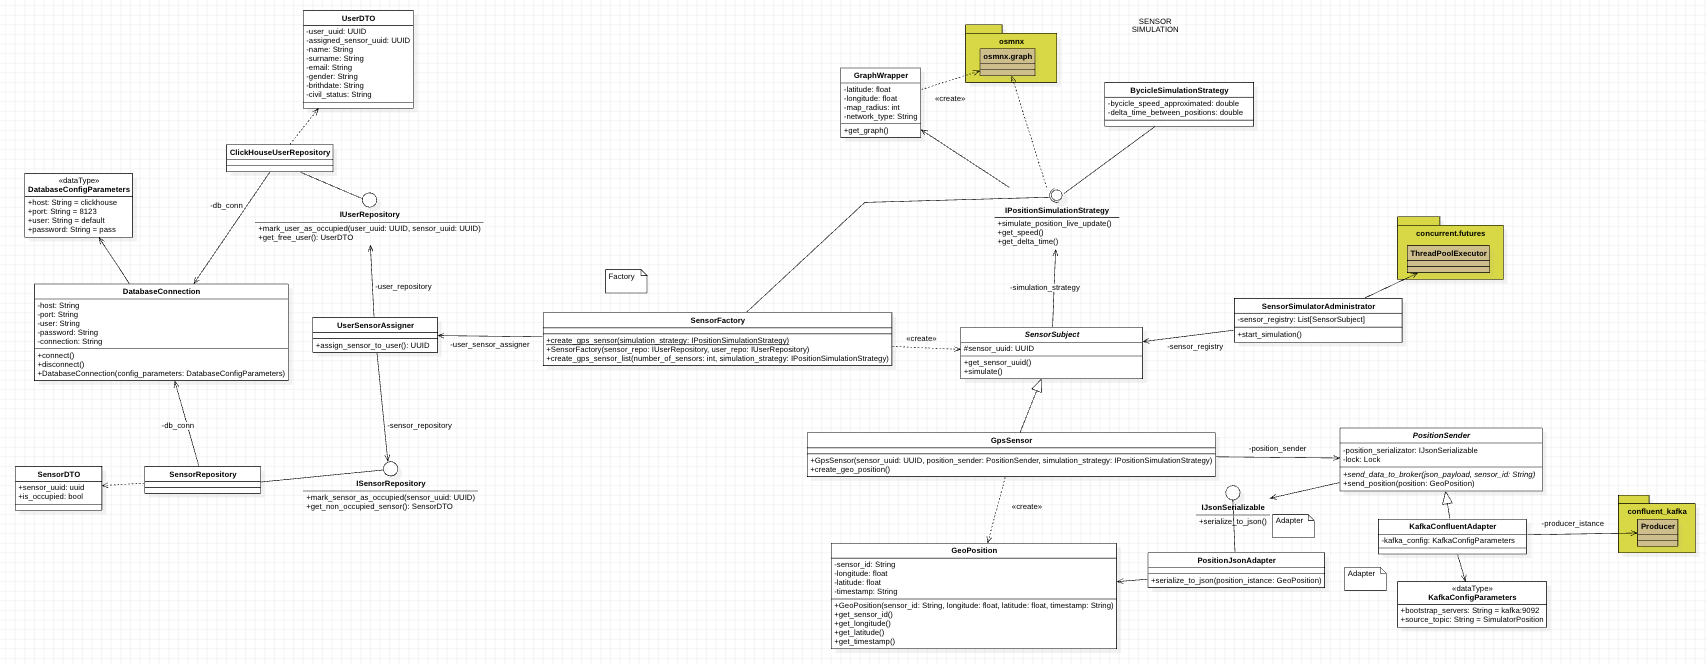
\includegraphics[width=0.8\textwidth]{diaSimulation.png}
    %     \caption{Diagramma delle classi del modulo di simulazione}
    %     \label{fig:simulation_module}
    % \end{figure}

    \paragraph{SensorFactory}
    \begin{itemize}
        \item \textbf{Descrizione}: Implementa il pattern Factory per la creazione di sensori GPS configurati. Si occupa di istanziare oggetti di tipo GpsSensor con le configurazioni appropriate, facilitando la gestione delle dipendenze.
        \item \textbf{Attributi}:
        \begin{itemize}
            \item \texttt{\_\_user\_sensor\_service: UserSensorService} - Servizio per l'assegnazione di sensori agli utenti, gestisce la corrispondenza tra UUID dei sensori e profili utente.
        \end{itemize}
        \item \textbf{Operazioni}:
        \begin{itemize}
            \item \texttt{\_\_init\_\_(self, sensor\_repo: ISensorRepository, user\_repo: IUserRepository)} - Costruttore che inizializza la factory con i repository necessari per sensori e utenti.
            \item \texttt{create\_gps\_sensor(self, position\_sender: PositionSender, simulation\_strategy: IPositionSimulationStrategy) -> SensorSubject} - Crea un singolo sensore GPS con il sender e la strategia forniti, generando un UUID unico.
            \item \texttt{create\_gps\_sensor\_list(self, position\_sender: PositionSender, simulation\_strategy: IPositionSimulationStrategy, number\_of\_sensors: int) -> List[SensorSubject]} - Crea una lista di sensori GPS con la configurazione specificata, utile per simulazioni multiple.
        \end{itemize}
    \end{itemize}

    \paragraph{GpsSensor}
    \begin{itemize}
        \item \textbf{Descrizione}: Implementa un sensore GPS che simula il movimento utilizzando la strategia fornita. Rappresenta un dispositivo fisico che trasmette dati di posizione.
        \item \textbf{Attributi}:
        \begin{itemize}
            \item \texttt{\_\_sensor\_uuid: str} - Identificatore univoco del sensore utilizzato per tracciare le posizioni.
            \item \texttt{\_\_position\_sender: PositionSender} - Componente responsabile dell'invio delle posizioni al sistema di messaggistica.
            \item \texttt{\_\_simulation\_strategy: IPositionSimulationStrategy} - Strategia utilizzata per simulare lo spostamento del sensore.
        \end{itemize}
        \item \textbf{Operazioni}:
        \begin{itemize}
            \item \texttt{\_\_init\_\_(self, sensor\_id: str, position\_sender: PositionSender, simulation\_strategy: IPositionSimulationStrategy)} - Inizializza il sensore con un ID, un sender e una strategia di simulazione.
            \item \texttt{simulate(self)} - Metodo principale che avvia la simulazione del movimento utilizzando la strategia definita, generando nuove posizioni a intervalli regolari.
            \item \texttt{create\_geo\_position(self, latitude: float, longitude: float, timestamp: str) -> GeoPosition} - Crea un oggetto posizione con le coordinate specificate e il timestamp corrente.
        \end{itemize}
    \end{itemize}

    \paragraph{SensorSubject}
    \begin{itemize}
        \item \textbf{Descrizione}: Interfaccia che definisce il contratto per gli oggetti di tipo sensore, implementa il pattern Observer per notificare i cambiamenti di posizione.
        \item \textbf{Operazioni}:
        \begin{itemize}
            \item \texttt{attach(self, observer: Observer)} - Registra un observer per ricevere notifiche dal sensore.
            \item \texttt{detach(self, observer: Observer)} - Rimuove un observer registrato.
            \item \texttt{notify(self)} - Notifica tutti gli observer registrati di un cambiamento di stato.
            \item \texttt{simulate(self)} - Metodo astratto che deve essere implementato dalle classi concrete per avviare la simulazione.
        \end{itemize}
    \end{itemize}

    \paragraph{PositionSender}
    \begin{itemize}
        \item \textbf{Descrizione}: Classe astratta che definisce l'interfaccia per l'invio delle posizioni attraverso vari canali di comunicazione.
        \item \textbf{Attributi}:
        \begin{itemize}
            \item \texttt{\_\_position\_serializator: IJsonSerializable} - Adattatore per la serializzazione in formato JSON.
            \item \texttt{\_lock: threading.Lock} - Lock per garantire thread safety durante l'invio di dati.
        \end{itemize}
        \item \textbf{Operazioni}:
        \begin{itemize}
            \item \texttt{\_\_init\_\_(self, json\_adapter\_istance: IJsonSerializable)} - Costruttore che inizializza il sender con l'istanza del serializzatore.
            \item \texttt{send\_data\_to\_broker(self, json\_payload, sensor\_id: str)} - Metodo astratto da implementare nelle sottoclassi per inviare dati al broker.
            \item \texttt{send\_position(self, position: GeoPosition)} - Metodo che serializza e invia una posizione utilizzando l'adapter fornito.
        \end{itemize}
    \end{itemize}

    \paragraph{KafkaConfluentAdapter}
    \begin{itemize}
        \item \textbf{Descrizione}: Implementazione concreta di PositionSender che utilizza Confluent Kafka per pubblicare i dati di posizione.
        \item \textbf{Attributi}:
        \begin{itemize}
            \item \texttt{\_\_kafka\_config: KafkaConfigParameters} - Configurazione per la connessione a Kafka, include host, porta e topic.
            \item \texttt{\_\_producer: Producer} - Producer Kafka utilizzato per l'invio dei messaggi.
        \end{itemize}
        \item \textbf{Operazioni}:
        \begin{itemize}
            \item \texttt{\_\_init\_\_(self, kafka\_config: KafkaConfigParameters, json\_adapter\_istance: PositionJsonAdapter, producer\_istance: Producer)} - Costruttore che inizializza l'adapter con la configurazione Kafka e il producer.
            \item \texttt{send\_data\_to\_broker(self, json\_payload, sensor\_id: str)} - Implementazione concreta che invia dati a Kafka utilizzando il producer configurato.
        \end{itemize}
    \end{itemize}

    \paragraph{IPositionSimulationStrategy}
    \begin{itemize}
        \item \textbf{Descrizione}: Interfaccia che definisce le strategie di simulazione del movimento, implementando il pattern Strategy.
        \item \textbf{Operazioni}:
        \begin{itemize}
            \item \texttt{get\_route(self)} - Ottiene il percorso da simulare, ritornando una sequenza di coordinate geografiche.
            \item \texttt{get\_delta\_time(self) -> float} - Ottiene l'intervallo di tempo in secondi tra aggiornamenti consecutivi di posizione.
            \item \texttt{get\_speed(self) -> float} - Ottiene la velocità di simulazione in km/h.
        \end{itemize}
    \end{itemize}

    \paragraph{BycicleSimulationStrategy}
    \begin{itemize}
        \item \textbf{Descrizione}: Implementazione concreta della strategia che simula il movimento di una bicicletta, generando percorsi realistici.
        \item \textbf{Attributi}:
        \begin{itemize}
            \item \texttt{\_\_osmnx\_graph: GraphWrapper} - Grafo stradale di OpenStreetMap utilizzato per la generazione di percorsi realistici.
        \end{itemize}
        \item \textbf{Operazioni}:
        \begin{itemize}
            \item \texttt{\_\_init\_\_(self, map\_graph: GraphWrapper)} - Costruttore che inizializza la strategia con un grafo stradale.
            \item \texttt{get\_route(self)} - Genera un percorso realistico utilizzando il grafo stradale, selezionando punti di partenza e arrivo casuali.
            \item \texttt{get\_delta\_time(self) -> float} - Restituisce l'intervallo temporale predefinito di 2 secondi tra aggiornamenti.
            \item \texttt{get\_speed(self) -> float} - Restituisce la velocità media simulata di 15 km/h tipica per una bicicletta.
        \end{itemize}
    \end{itemize}

    \paragraph{SensorSimulationAdministrator}
    \begin{itemize}
        \item \textbf{Descrizione}: Coordina la simulazione di più sensori in parallelo, gestendo l'esecuzione concorrente.
        \item \textbf{Attributi}:
        \begin{itemize}
            \item \texttt{\_\_sensor\_registry: List[SensorSubject]} - Registro contenente tutti i sensori da simulare.
            \item \texttt{\_\_executor: ThreadPoolExecutor} - Pool di thread per l'esecuzione parallela delle simulazioni.
        \end{itemize}
        \item \textbf{Operazioni}:
        \begin{itemize}
            \item \texttt{\_\_init\_\_(self, list\_of\_sensors: List[SensorSubject])} - Costruttore che inizializza l'amministratore con una lista di sensori.
            \item \texttt{start\_simulation(self)} - Avvia la simulazione per tutti i sensori registrati utilizzando un thread pool.
            \item \texttt{stop\_simulation(self)} - Arresta la simulazione in corso per tutti i sensori.
        \end{itemize}
    \end{itemize}

    \paragraph{GeoPosition}
    \begin{itemize}
        \item \textbf{Descrizione}: Classe che rappresenta una posizione geografica con coordinate e timestamp.
        \item \textbf{Attributi}:
        \begin{itemize}
            \item \texttt{\_\_sensor\_id: str} - Identificatore del sensore che ha generato la posizione.
            \item \texttt{\_\_latitude: float} - Latitudine della posizione in gradi decimali.
            \item \texttt{\_\_longitude: float} - Longitudine della posizione in gradi decimali.
            \item \texttt{\_\_timestamp: str} - Timestamp ISO 8601 che indica quando è stata rilevata la posizione.
        \end{itemize}
        \item \textbf{Operazioni}:
        \begin{itemize}
            \item \texttt{get\_sensor\_id(self) -> str} - Restituisce l'ID del sensore associato.
            \item \texttt{get\_latitude(self) -> float} - Restituisce la latitudine.
            \item \texttt{get\_longitude(self) -> float} - Restituisce la longitudine.
            \item \texttt{get\_timestamp(self) -> str} - Restituisce il timestamp della rilevazione.
        \end{itemize}
    \end{itemize}

    \subsubsection{Processore Flink}
    Il processore Flink è responsabile dell'elaborazione dei dati di posizione in tempo reale per generare messaggi pubblicitari personalizzati.

    % \begin{figure}[H]
    %     \centering
    %     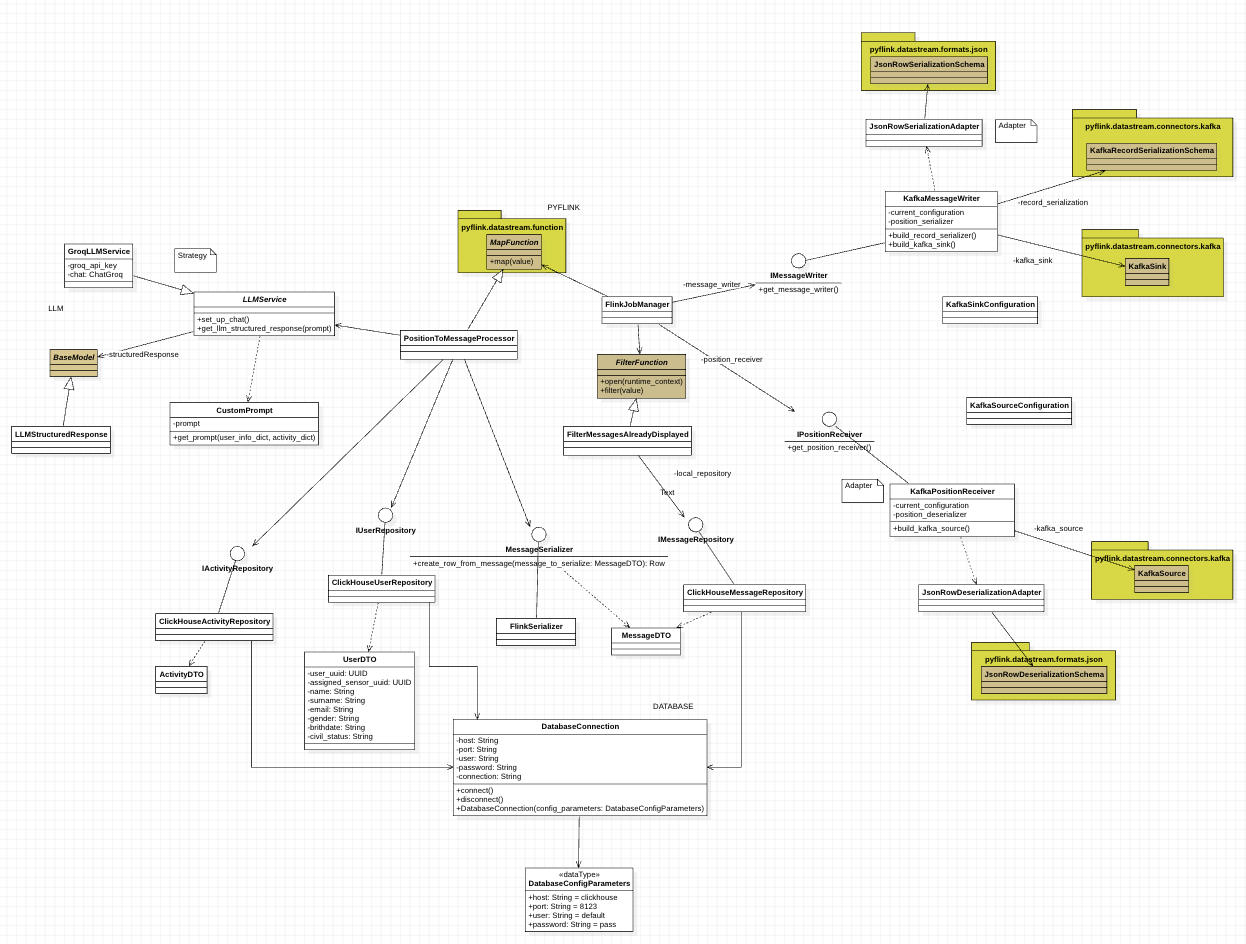
\includegraphics[width=0.8\textwidth]{diaFlink.png}
    %     \caption{Diagramma delle classi del processore Flink}
    %     \label{fig:flink_processor}
    % \end{figure}

    \paragraph{FlinkJobManager}
    \begin{itemize}
        \item \textbf{Descrizione}: Coordina l'esecuzione del job Flink, definendo il flusso di elaborazione dei dati e orchestrando le diverse trasformazioni.
        \item \textbf{Attributi}:
        \begin{itemize}
            \item \texttt{\_\_streaming\_env: StreamExecutionEnvironment} - Ambiente di esecuzione Flink per la definizione e l'esecuzione del job.
            \item \texttt{\_\_populated\_datastream} - Stream di dati iniziale proveniente dalla source Kafka.
            \item \texttt{keyed\_stream} - Stream con chiave applicata, utilizzato per raggruppare dati relativi allo stesso sensore/utente.
            \item \texttt{\_\_mapped\_stream} - Stream risultante dopo l'applicazione della map function.
            \item \texttt{\_\_filtered\_stream} - Stream finale dopo l'applicazione della funzione di filtro.
        \end{itemize}
        \item \textbf{Operazioni}:
        \begin{itemize}
            \item \texttt{\_\_init\_\_(self, streaming\_env\_istance: StreamExecutionEnvironment, map\_function\_implementation: MapFunction, filter\_function\_implementation: FilterFunction, position\_receiver\_istance: IPositionReceiver, message\_sender\_istance: IMessageWriter)} - Costruttore che configura il job con l'ambiente e le funzioni di trasformazione.
            \item \texttt{execute(self)} - Esegue il job Flink, avviando l'elaborazione e mantenendola attiva.
        \end{itemize}
    \end{itemize}

    \paragraph{PositionToMessageProcessor}
    \begin{itemize}
        \item \textbf{Descrizione}: Implementa la MapFunction di Flink per trasformare le posizioni in messaggi pubblicitari personalizzati.
        \item \textbf{Attributi}:
        \begin{itemize}
            \item \texttt{ai\_service: LLMService} - Servizio LLM per generare messaggi pubblicitari contestuali.
            \item \texttt{\_\_user\_repository: IUserRepository} - Repository per accedere ai dati utente, come preferenze e informazioni demografiche.
            \item \texttt{\_\_activity\_repository: IActivityRepository} - Repository per accedere ai dati delle attività commerciali nelle vicinanze.
            \item \texttt{\_\_message\_serializer: IFlinkSerializable} - Serializer per i messaggi generati che saranno inviati a Kafka.
        \end{itemize}
        \item \textbf{Operazioni}:
        \begin{itemize}
            \item \texttt{\_\_init\_\_(self, ai\_chatbot\_service: LLMService, user\_repository: IUserRepository, activity\_repository: IActivityRepository, message\_serializer: IFlinkSerializable)} - Costruttore che inizializza il processore con i servizi necessari.
            \item \texttt{open(self, runtime\_context)} - Inizializza il servizio LLM e altre risorse necessarie durante l'avvio del task.
            \item \texttt{map(self, value)} - Trasforma un record di posizione in un messaggio pubblicitario, identificando POI nelle vicinanze e generando contenuti personalizzati.
        \end{itemize}
    \end{itemize}

    \paragraph{FilterMessageAlreadyDisplayed}
    \begin{itemize}
        \item \textbf{Descrizione}: Implementa FilterFunction per evitare duplicazioni di messaggi per lo stesso utente entro un certo periodo di tempo.
        \item \textbf{Attributi}:
        \begin{itemize}
            \item \texttt{\_\_message\_repository: IMessageRepository} - Repository per verificare l'esistenza di messaggi precedenti.
        \end{itemize}
        \item \textbf{Operazioni}:
        \begin{itemize}
            \item \texttt{\_\_init\_\_(self, message\_repository: IMessageRepository)} - Costruttore che inizializza il filtro con il repository dei messaggi.
            \item \texttt{filter(self, value)} - Filtra i messaggi che sono già stati visualizzati dall'utente per la stessa attività entro un periodo configurabile.
        \end{itemize}
    \end{itemize}

    \paragraph{KafkaPositionReceiver}
    \begin{itemize}
        \item \textbf{Descrizione}: Adattatore per ricevere posizioni da Kafka, implementa IPositionReceiver.
        \item \textbf{Attributi}:
        \begin{itemize}
            \item \texttt{\_\_current\_configuration: KafkaSourceConfiguration} - Configurazione della source Kafka, inclusi topic, gruppo di consumer e server.
            \item \texttt{\_\_position\_deserializer} - Deserializzatore per convertire i dati JSON in oggetti utilizzabili.
            \item \texttt{\_\_kafka\_source: KafkaSource} - Source Kafka configurata per la lettura dei dati.
        \end{itemize}
        \item \textbf{Operazioni}:
        \begin{itemize}
            \item \texttt{\_\_init\_\_(self, kafka\_source\_configuration: KafkaSourceConfiguration, deserialize\_adapter: JsonRowDeserializationAdapter)} - Costruttore che inizializza il receiver con la configurazione e il deserializzatore.
            \item \texttt{build\_kafka\_source(self) -> KafkaSource} - Costruisce e configura la source Kafka con le impostazioni appropriate.
            \item \texttt{get\_position\_receiver(self)} - Restituisce la source Kafka configurata per l'utilizzo nel job Flink.
        \end{itemize}
    \end{itemize}

    \paragraph{KafkaMessageWriter}
    \begin{itemize}
        \item \textbf{Descrizione}: Adattatore per scrivere messaggi su Kafka, implementa IMessageWriter.
        \item \textbf{Attributi}:
        \begin{itemize}
            \item \texttt{\_\_current\_configuration: KafkaWriterConfiguration} - Configurazione del writer Kafka, inclusi topic e server.
            \item \texttt{\_\_position\_serializer} - Serializzatore per convertire gli oggetti in formato JSON.
            \item \texttt{\_\_record\_serializer} - Serializzatore per i record Kafka, gestisce la trasformazione e la definizione di schema.
            \item \texttt{\_\_kafka\_sink: KafkaSink} - Sink Kafka configurata per la scrittura dei dati.
        \end{itemize}
        \item \textbf{Operazioni}:
        \begin{itemize}
            \item \texttt{\_\_init\_\_(self, kafka\_writer\_configuration: KafkaWriterConfiguration, serialize\_adapter: JsonRowSerializationAdapter)} - Costruttore che inizializza il writer con la configurazione e il serializzatore.
            \item \texttt{build\_record\_serializer(self)} - Costruisce il serializzatore di record per Kafka.
            \item \texttt{build\_kafka\_sink(self)} - Costruisce la sink Kafka con le impostazioni appropriate.
            \item \texttt{get\_message\_writer(self)} - Restituisce la sink Kafka configurata per l'utilizzo nel job Flink.
        \end{itemize}
    \end{itemize}

    \paragraph{LLMService}
    \begin{itemize}
        \item \textbf{Descrizione}: Classe astratta che definisce l'interfaccia per i servizi di language model utilizzati nella generazione di messaggi personalizzati.
        \item \textbf{Attributi}:
        \begin{itemize}
            \item \texttt{\_llm\_structured\_response: BaseModel} - Modello Pydantic per la risposta strutturata proveniente dal LLM.
        \end{itemize}
        \item \textbf{Operazioni}:
        \begin{itemize}
            \item \texttt{\_\_init\_\_(self, structured\_response: BaseModel)} - Costruttore che inizializza il servizio con il modello di risposta strutturata.
            \item \texttt{set\_up\_chat(self)} - Metodo astratto per inizializzare la connessione con il servizio LLM.
            \item \texttt{get\_llm\_structured\_response(self, prompt)} - Metodo astratto per ottenere una risposta strutturata dall'LLM.
        \end{itemize}
    \end{itemize}

    \paragraph{GroqLLMService}
    \begin{itemize}
        \item \textbf{Descrizione}: Implementazione concreta di LLMService che utilizza il provider Groq per la generazione di testi.
        \item \textbf{Attributi}:
        \begin{itemize}
            \item \texttt{\_\_groq\_api\_key: str} - Chiave API per l'autenticazione con il servizio Groq.
            \item \texttt{\_\_chat} - Istanza del client Groq per l'interazione con il servizio.
        \end{itemize}
        \item \textbf{Operazioni}:
        \begin{itemize}
            \item \texttt{\_\_init\_\_(self, structured\_response: BaseModel)} - Costruttore che inizializza il servizio Groq.
            \item \texttt{set\_up\_chat(self)} - Configura il client Groq con rate limiting e gestione degli errori.
            \item \texttt{get\_llm\_structured\_response(self, prompt)} - Invia un prompt al servizio Groq e converte la risposta in un formato strutturato.
        \end{itemize}
    \end{itemize}

    \paragraph{MessageDTO}
    \begin{itemize}
        \item \textbf{Descrizione}: Data Transfer Object per i messaggi pubblicitari generati.
        \item \textbf{Attributi}:
        \begin{itemize}
            \item \texttt{user\_uuid: str} - Identificatore univoco dell'utente destinatario.
            \item \texttt{activity\_uuid: str} - Identificatore univoco dell'attività commerciale associata.
            \item \texttt{message\_uuid: str} - Identificatore univoco del messaggio.
            \item \texttt{message: str} - Contenuto testuale del messaggio pubblicitario.
            \item \texttt{activityLatitude: float} - Latitudine dell'attività commerciale.
            \item \texttt{activityLongitude: float} - Longitudine dell'attività commerciale.
            \item \texttt{creationTime: str} - Timestamp di creazione del messaggio.
            \item \texttt{userLatitude: float} - Latitudine dell'utente al momento della generazione.
            \item \texttt{userLongitude: float} - Longitudine dell'utente al momento della generazione.
        \end{itemize}
    \end{itemize}

    \paragraph{ActivityDTO}
    \begin{itemize}
        \item \textbf{Descrizione}: Data Transfer Object per le attività commerciali.
        \item \textbf{Attributi}:
        \begin{itemize}
            \item \texttt{activity\_id: str} - Identificatore univoco dell'attività.
            \item \texttt{name: str} - Nome dell'attività commerciale.
            \item \texttt{category: str} - Categoria o tipologia dell'attività.
            \item \texttt{description: str} - Descrizione dettagliata dell'attività.
            \item \texttt{latitude: float} - Latitudine dell'attività.
            \item \texttt{longitude: float} - Longitudine dell'attività.
        \end{itemize}
    \end{itemize}

    \paragraph{UserDTO}
    \begin{itemize}
        \item \textbf{Descrizione}: Data Transfer Object per gli utenti del sistema.
        \item \textbf{Attributi}:
        \begin{itemize}
            \item \texttt{user\_id: str} - Identificatore univoco dell'utente.
            \item \texttt{name: str} - Nome dell'utente.
            \item \texttt{age: int} - Età dell'utente.
            \item \texttt{gender: str} - Genere dell'utente.
            \item \texttt{interests: List[str]} - Lista degli interessi dell'utente.
            \item \texttt{preferences: List[str]} - Lista delle preferenze dell'utente.
        \end{itemize}
    \end{itemize}

    \subsubsection{Relazioni tra componenti}
    Le relazioni tra i componenti riflettono l'architettura modulare del sistema, basata su interfacce che seguono i principi SOLID:

    \paragraph{Modulo di Simulazione}
    \begin{itemize}
        \item \texttt{SensorFactory} crea istanze di \texttt{GpsSensor} che implementano l'interfaccia \texttt{SensorSubject}.
        \item \texttt{GpsSensor} utilizza \texttt{IPositionSimulationStrategy} (implementata da \texttt{BycicleSimulationStrategy}) per determinare il proprio movimento.
        \item \texttt{GpsSensor} invia dati attraverso \texttt{PositionSender} (implementato da \texttt{KafkaConfluentAdapter}) che utilizza \texttt{IJsonSerializable} per la serializzazione.
        \item \texttt{SensorSimulationAdministrator} coordina una collezione di sensori che implementano \texttt{SensorSubject}.
    \end{itemize}

    \paragraph{Processore Flink}
    \begin{itemize}
        \item \texttt{FlinkJobManager} orchestra l'intero flusso di elaborazione, ricevendo dati tramite \texttt{KafkaPositionReceiver} (implementa \texttt{IPositionReceiver}).
        \item \texttt{FlinkJobManager} applica \texttt{PositionToMessageProcessor} per trasformare i dati (implementa \texttt{MapFunction}) e \texttt{FilterMessageAlreadyDisplayed} per filtrare messaggi duplicati (implementa \texttt{FilterFunction}).
        \item \texttt{FlinkJobManager} invia i risultati tramite \texttt{KafkaMessageWriter} (implementa \texttt{IMessageWriter}).
        \item \texttt{PositionToMessageProcessor} interagisce con \texttt{LLMService} (implementato da \texttt{GroqLLMService}) per generare messaggi, e con repository di dati per accedere a informazioni su utenti e attività.
    \end{itemize}

    Questa architettura modulare consente un alto grado di testabilità e manutenibilità, permettendo la sostituzione di componenti con implementazioni alternative senza modificare il flusso di elaborazione complessivo.

\newpage
\section{Architettura di deployment}
Da capitolato era stato definito l'uso di un'architettura containerizzata e anche valutando alcune alternative risultava comunque la scelta più ragionevole. Al fine di implementare ed eseguire l'intero stack tecnologico ed i componenti del modello architetturale del sistema seguendo questa architettura, è stato configurato un ambiente Docker che simula la suddivisione e la distribuzione dei servizi. Informazioni aggiuntive sulle immagini utilizzate e sulle configurazioni dell'ambiente sono disponibili nel file docker-compose.yml presente nel repository del progetto oltre che nella sezione \ref{sec:strumenti}.
    \subsection{Panoramica dell'infrastruttura}
        \subsubsection{Ambiente Docker}
        Descrizione dell'ambiente Docker utilizzato, incluse le immagini e le configurazioni specifiche.

        \subsubsection{Componenti principali}
        In questa sezione vengono descritti i componenti principali dell'architettura, evidenziandone i ruoli e le responsabilità.

        \subsubsection{Dipendenze tra componenti}
        Le interazioni tra i vari componenti avvengono attraverso Kafka, che garantisce l'invio e la ricezione di messaggi in modo affidabile e resiliente.

\begin{itemize}
    \item \textbf{Generazione di dati:}
    \begin{itemize}
        \item \textbf{Container sensor-simulator:}
        \begin{itemize}
            \item[.] Esegue il simulatore dei sensori di posizione degli utenti;
            \item[.] Implementa diverse strategie di movimento per generare dati realistici;
            \item[.] Produce dati nel formato JSON definito e li invia al broker Kafka.
        \end{itemize}
    \end{itemize}

    \item \textbf{Gestione messaggi:}
    \begin{itemize}
        \item \textbf{Container kafka:}
        \begin{itemize}
            \item[.] Esegue Apache Kafka per la gestione del flusso di dati in tempo reale;
            \item[.] Gestisce i topic dedicati per i diversi tipi di messaggi (posizioni, POI, messaggi pubblicitari);
            \item[.] Accessibile agli altri container tramite l'indirizzo kafka:9092.
        \end{itemize}
        \item \textbf{Componenti di supporto:}
        \begin{itemize}
            \item[.] \textbf{Container zookeeper:}
            \begin{itemize}
                \item[-] Esegue il servizio di coordinamento per Kafka;
                \item[-] Gestisce lo stato distribuito del sistema;
                \item[-] Accessibile dagli altri container attraverso l'indirizzo zookeeper:2181.
            \end{itemize}
            \item[.] \textbf{Container kafka-ui:}
            \begin{itemize}
                \item[-] Fornisce un'interfaccia web per il monitoraggio e la gestione di Kafka;
                \item[-] Espone la porta 8080 per accedere alla dashboard di amministrazione.
            \end{itemize}
        \end{itemize}
    \end{itemize}

    \item \textbf{Elaborazione dei dati:}
    \begin{itemize}
        \item \textbf{Container flink-jobmanager:}
        \begin{itemize}
            \item[.] Coordina l'esecuzione dei job di elaborazione dati in tempo reale;
            \item[.] Gestisce l'allocazione delle risorse e la pianificazione dei task;
            \item[.] Espone la porta 8081 per l'interfaccia di amministrazione.
        \end{itemize}
        \item \textbf{Container flink-taskmanager:}
        \begin{itemize}
            \item[.] Esegue i task di elaborazione dati assegnati dal jobmanager;
            \item[.] Implementa gli algoritmi di proximity detection per identificare punti di interesse rilevanti;
            \item[.] Integra il servizio LLM per la generazione di messaggi pubblicitari personalizzati.
        \end{itemize}
    \end{itemize}

    \item \textbf{Storage:}
    \begin{itemize}
        \item \textbf{Container clickhouse:}
        \begin{itemize}
            \item[.] Esegue ClickHouse come database column-oriented ad alte prestazioni;
            \item[.] Memorizza i dati degli utenti, posizioni, punti di interesse e messaggi pubblicitari;
            \item[.] La banca dati è accessibile agli altri container tramite l'indirizzo clickhouse:8123 e 9000.
        \end{itemize}
    \end{itemize}

    \item \textbf{Visualizzazione:}
    \begin{itemize}
        \item \textbf{Container grafana:}
        \begin{itemize}
            \item[.] Esegue Grafana come piattaforma di visualizzazione e monitoraggio;
            \item[.] Offre dashboard interattive per l'analisi dei dati di posizione e messaggi pubblicitari;
            \item[.] Espone la porta 3000 all'esterno per permettere l'accesso alle dashboard;
            \item[.] Consente l'integrazione con vari datasource per la visualizzazione dei dati.
        \end{itemize}
    \end{itemize}
\end{itemize}

\subsection{Vantaggi dell'architettura containerizzata}
Questa struttura containerizzata permette una distribuzione modulare e scalabile del sistema, semplificando la gestione e la manutenzione dei componenti e consentendo una rapida scalabilità in risposta alle esigenze emergenti. Grazie all'uso di Docker, si garantisce:

\begin{itemize}
    \item \textbf{Isolamento}: Ogni componente opera nel proprio ambiente isolato, riducendo le interferenze tra servizi;
    \item \textbf{Portabilità}: L'applicazione può essere eseguita su qualsiasi piattaforma che supporti Docker;
    \item \textbf{Portabilità della configurazione}: Grazie al compose di Docker si possono definire delle cartelle o dei file di configurazione per ogni container, rendendo il sistema facilmente replicabile;
    \item \textbf{Scalabilità orizzontale}: I container possono essere facilmente replicati per gestire carichi maggiori;
    \item \textbf{Gestione dichiarativa}: La configurazione dell'intero ambiente è definita nel file docker-compose.yml;
    \item \textbf{Efficienza delle risorse}: Ogni container riceve solo le risorse necessarie per il suo funzionamento.
\end{itemize}

\subsection{Comunicazione tra container}
La comunicazione tra i vari container avviene principalmente attraverso il networking interno di Docker, con Kafka che agisce come backbone di messaggistica centrale del sistema. Questa architettura event-driven garantisce:

\begin{itemize}
    \item \textbf{Disaccoppiamento}: I componenti possono evolvere indipendentemente, purché mantengano l'interfaccia di comunicazione;
    \item \textbf{Persistenza dei messaggi}: I dati vengono memorizzati in Kafka e copiati subito dopo su una tabella ClickHouse, garantendo la storicizzazione del dato.
\end{itemize}

\subsection{Orchestrazione e gestione}
Per la gestione dei container in ambiente di produzione, sono state implementate le seguenti strategie:

\begin{itemize}
    \item \textbf{Health checks}: Ogni container è configurato con controlli di integrità che verificano periodicamente il corretto funzionamento del servizio;
    \item \textbf{Gerarchia di avvio dei container}: I container vengono avviati in un ordine specifico per garantire che le dipendenze siano soddisfatte prima di avviare i servizi che ne fanno uso.
\end{itemize}

\subsection{Evoluzione futura}
L'architettura di deployment containerizzato con la sua separazione degli ambienti offre facile implementazione di future evoluzioni del sistema, tra cui:

\begin{itemize}
    \item \textbf{Migrazione verso Kubernetes}: L'attuale configurazione Docker è pronta per essere eventualmente trasferita su un orchestratore come Kubernetes per una gestione più avanzata dei container;
    \item \textbf{Implementazione di auto-scaling}: Aggiunta di meccanismi per scalare automaticamente i servizi in base al carico;
    \item \textbf{Monitoraggio}: C'è la possibilità di integrare strumenti di monitoraggio avanzati per analizzare le performance e il comportamento del sistema in tempo reale.
\end{itemize}

\newpage

\section{Stato dei requisiti funzionali}

La presente sezione fornisce una visione d'insieme dello stato di avanzamento dei requisiti funzionali identificati durante la fase di analisi. I requisiti funzionali sono stati classificati in base alla loro importanza (obbligatori, desiderabili e opzionali) come definito nel documento \textit{Analisi\_dei\_Requisiti\_v1.0.0}.

\subsection{Riepilogo dei requisiti}
Durante la fase di analisi sono stati individuati 33 requisiti funzionali (RF01-RF33), di cui:
\begin{itemize}
    \item 27 requisiti obbligatori;
    \item 0 requisiti desiderabili;
    \item 2 requisiti opzionali.
\end{itemize}

I requisiti funzionali riguardano principalmente:
\begin{itemize}
    \item La visualizzazione della Dashboard e dei Marker sulla mappa;
    \item La gestione e visualizzazione dei punti di interesse;
    \item La visualizzazione degli annunci pubblicitari generati;
    \item La trasmissione e gestione dei dati geoposizionali.
\end{itemize}

\subsection{Tabella dei requisiti funzionali}

\begin{longtable}{|>{\centering\arraybackslash}m{2.7cm}|>{\centering\arraybackslash}m{2.7cm}|>{\raggedright\arraybackslash}m{6cm}|>{\centering\arraybackslash}m{2.1cm}|}
    \hline
    \rowcolor{gray!25}
    \textbf{Id. Requisito} & \textbf{Importanza} & \textbf{Descrizione} & \textbf{Stato}\\
    \hline
    RF01 & Obbligatorio & L'utente privilegiato deve poter visualizzare la Dashboard composta da una mappa interattiva con i vari Marker su di essa. & Implementato \\
    \hline
    RF02 & Obbligatorio & L'utente privilegiato deve poter visualizzare dei Marker che rappresentano i vari Percorsi effettuati in tempo reale dagli utenti presenti nel Sistema & Implementato \\
    \hline
    RF03 & Obbligatorio & L'utente privilegiato deve poter visualizzare un Marker che rappresenta un Percorso effettuato in tempo reale da un utente presente nel Sistema & Implementato \\
    \hline
    RF04 & Obbligatorio & L'utente privilegiato deve poter visualizzare tutti i punti di interesse riconosciuti dal Sistema. & Implementato \\
    \hline
    RF05 & Obbligatorio & L'utente privilegiato deve poter visualizzare un Marker che rappresenta un punto di interesse riconosciuto dal Sistema. & Implementato \\
    \hline
    RF06 & Obbligatorio & L'utente privilegiato deve poter visualizzare gli annunci pubblicitari provenienti da un determinato punto di interesse. & Implementato \\
    \hline
    RF07 & Obbligatorio & L'utente privilegiato deve poter visualizzare un singolo annuncio pubblicitario tramite un Marker. & Implementato \\
    \hline
    RF08 & Obbligatorio & L'utente privilegiato deve poter visualizzare una Dashboard relativa ad un singolo utente quando seleziona un Marker utente nella Dashboard principale. & Implementato \\
    \hline
    RF09 & Obbligatorio & L'utente privilegiato deve poter visualizzare dei Marker che rappresentano lo storico delle posizioni dell'utente a cui è riferita la Dashboard di singolo utente. & Implementato \\
    \hline
    RF10 & Obbligatorio & L'utente privilegiato deve poter visualizzare un Marker che rappresenta la posizione dell'utente in un determinato istante nella Dashboard di singolo utente. & Implementato \\
    \hline
    RF11 & Obbligatorio & L'utente privilegiato deve poter visualizzare, nella Dashboard di singolo utente, tutti i punti di interesse riconosciuti dal Sistema. & Implementato \\
    \hline
    RF12 & Obbligatorio & L'utente privilegiato deve poter visualizzare, nella Dashboard di singolo utente, un Marker che rappresenta un punto di interesse riconosciuto dal Sistema. & Implementato \\
    \hline
    RF13 & Obbligatorio & L'utente privilegiato deve poter visualizzare lo storico degli annunci pubblicitari generati per l'utente a cui è riferita la Dashboard singolo utente. & Implementato \\
    \hline
    RF14 & Obbligatorio & L'utente privilegiato deve poter visualizzare un singolo annuncio pubblicitario tramite un Marker nella Dashboard di singolo utente. & Implementato \\
    \hline
    RF15 & Obbligatorio & L'utente privilegiato deve poter visualizzare un pannello apposito contenente le informazioni dell'utente, a cui è riferita la Dashboard di singolo utente, in forma tabellare. & Implementato \\
    \hline
    RF16 & Obbligatorio & L'utente privilegiato deve poter visualizzare nel pannello apposito di visualizzazione informazioni dell'utente: il nome, il cognome, l'email, il genere, la data di nascita e lo stato civile. & Implementato \\
    \hline
    RF17 & Obbligatorio & L'utente privilegiato deve poter visualizzare i dettagli del Marker riguardante una singola posizione di un utente nella rispettiva Dashboard & Implementato \\
    \hline
    RF18 & Obbligatorio & L'utente privilegiato quando visualizza i dettagli del Marker, riguardante una singola posizione di un utente nella rispettiva Dashboard, deve poter vedere la latitudine, la longitudine e l'istante di rilevamento del Marker & Implementato \\
    \hline
    RF19 & Opzionale & L'utente privilegiato deve poter visualizzare l'area di influenza di un punto di interesse selezionato. & Implementato \\
    \hline
    RF20 & Obbligatorio & L'utente privilegiato deve poter visualizzare le informazioni dettagliate di un punto di interesse quando selezionato. & Implementato \\
    \hline
    RF21 & Obbligatorio & L'utente privilegiato quando visualizza le informazioni dettagliate di un punto di interesse deve poter visualizzare la latitudine, la longitudine, il nome, la tipologia e la descrizione del punto di interesse. & Implementato \\
    \hline
    RF22 & Opzionale & L'utente deve poter visualizzare l'annuncio pubblicitario proveniente dal punto di interesse situato nell'area che sta attraversando. & Da implementare \\
    \hline
    RF23 & Obbligatorio & L'utente privilegiato deve poter visualizzare una tabella contenente le informazioni dei singoli PoI ordinati per la quantità di messaggi inviati nel mese. & Implementato \\
    \hline
    RF24 & Obbligatorio & L'utente privilegiato deve poter visualizzare nella tabella dei PoI un singolo PoI, rappresentato da una riga della tabella. & Implementato \\
    \hline
    RF25 & Obbligatorio & L'utente privilegiato deve poter visualizzare in ogni riga della tabella dei PoI il nome, l'indirizzo, la tipologia (di che ambito si occupa), la descrizione e il numero di messaggi inviati durante il mese di un singolo PoI. & Implementato \\
    \hline
    RF26 & Obbligatorio & L'utente privilegiato deve poter visualizzare i dettagli di un annuncio generato. & Implementato \\
    \hline
    RF27 & Obbligatorio & L'utente privilegiato quando visualizza i dettagli di un annuncio deve poter visualizzare la latitudine, la longitudine, l'istante di creazione, il nome dell'utente coinvolto, il nome del punto di interesse coinvolto e il contenuto dell'annuncio. & Implementato \\
    \hline
    RF28 & Obbligatorio & Il sensore deve essere in grado di trasmettere i dati rilevati in tempo reale al Sistema. & Implementato \\
    \hline
    RF29 & Obbligatorio & Il sensore deve essere in grado di trasmettere il proprio id, la sua latitudine e longitudine al Sistema. & Implementato \\
    \hline
    RF30 & Obbligatorio & Il servizio LLM deve essere in grado di ricevere i dati dell'utente e del punto di interesse inviati dal Sistema. & In implementazione \\
    \hline
    RF31 & Obbligatorio & Il servizio LLM deve essere in grado di ricevere le informazioni dell'utente inviate dal Sistema, quali: il nome, il cognome, l'email, il genere, la data di nascita, lo stato civile e i suoi interessi. & In implementazione \\
    \hline
    RF32 & Obbligatorio & Il servizio LLM deve essere in grado di ricevere le informazioni del punto di interesse inviate dal Sistema, quali: il nome, l'indirizzo, la tipologia, la descrizione e la distanza del PoI dall'utente. & In implementazione \\
    \hline
    RF33 & Obbligatorio & Il servizio LLM deve essere in grado di trasmettere un messaggio custom, rappresentante il contenuto dell'annuncio per un utente, al Sistema. & Da implementare \\
    \hline
\end{longtable}

\subsection{Stato di implementazione}

Lo stato di implementazione dei requisiti funzionali è rappresentato nella seguente tabella:

\begin{table}[H]
\centering
\renewcommand{\arraystretch}{1.5}
\rowcolors{0}{gray!11}{white}
\begin{tabular}{|>{\centering\arraybackslash}m{2.5cm}|>{\centering\arraybackslash}m{2.5cm}|>{\centering\arraybackslash}m{2.5cm}|>{\centering\arraybackslash}m{2.5cm}|>{\centering\arraybackslash}m{2.5cm}|}
\hline
\rowcolor{gray!25}
\textbf{Tipo di requisito} & \textbf{Totale} & \textbf{Implementati} & \textbf{In implementazione} & \textbf{Da implementare} \\
\hline
Obbligatori & 31 & 26 & 3 & 2 \\
\hline
Desiderabili & 0 & 0 & 0 & 0 \\
\hline
Opzionali & 2 & 1 & 0 & 1 \\
\hline
\textbf{Totale} & 33 & 27 & 3 & 3 \\
\hline
\end{tabular}
\caption{Stato di implementazione dei requisiti funzionali}
\label{tab:stato_implementazione_requisiti}
\end{table}

\begin{figure}[H]
    \centering
    \begin{tikzpicture}
        \pie{84/Implementati, 10/In implementazione, 6/Da implementare}
    \end{tikzpicture}
    \caption{Stato dei requisiti funzionali obbligatori}
    \label{fig:stato_requisiti_obbligatori}
\end{figure}

\begin{figure}[H]
    \centering
    \begin{tikzpicture}
        \pie{82/Implementati, 9/In implementazione, 9/Da implementare}
    \end{tikzpicture}
    \caption{Stato dei requisiti funzionali totali}
    \label{fig:stato_requisiti_totali}
\end{figure}

\subsection{Conclusioni}

L'analisi dello stato dei requisiti funzionali indica un buon progresso nell'implementazione delle funzionalità richieste. Con l'82\% dei requisiti funzionali già implementati e il 9\% in fase di implementazione, il progetto è sulla buona strada per soddisfare tutti i requisiti obbligatori entro la consegna finale.

I requisiti attualmente in fase di implementazione riguardano principalmente l'integrazione con il servizio LLM, mentre quelli ancora da implementare comprendono uno dei requisiti opzionali e alcuni aspetti avanzati del sistema. La stabilità raggiunta nei requisiti dopo la revisione tecnica fornisce una base solida per il completamento dell'implementazione, mentre il sistema di test definito garantirà la qualità del prodotto finale.


\end{document}
